%%% main.tex — ICE-UTxO: Interleaving Coroutine Effects for Proof-Carrying UTxO Transactions
\documentclass[11pt,a4paper]{article}
\usepackage[margin=1in]{geometry}
\usepackage{hyperref}
\usepackage{xcolor}

%%% ── Packages ──────────────────────────────────────────────────────────────
\usepackage{amsmath}
\usepackage{amssymb}
\usepackage{mathtools}
\usepackage{stmaryrd}
\usepackage{tikz}
\usepackage{listings}
\usepackage{booktabs}
\usepackage{adjustbox}
\usepackage{cleveref}

%%% ── TikZ libraries ───────────────────────────────────────────────────────
\usetikzlibrary{positioning,arrows.meta,shapes,fit,backgrounds,automata,calc,
                 patterns,decorations.pathreplacing}

%%% ── Shared colour palette (Material Design, desaturated for academic use) ──
\definecolor{palBlue}{HTML}{1976D2}
\definecolor{palBlueLt}{HTML}{E3F2FD}
\definecolor{palGreen}{HTML}{388E3C}
\definecolor{palGreenLt}{HTML}{E8F5E9}
\definecolor{palOrange}{HTML}{E65100}
\definecolor{palOrangeLt}{HTML}{FFF3E0}
\definecolor{palPurple}{HTML}{7B1FA2}
\definecolor{palPurpleLt}{HTML}{F3E5F5}
\definecolor{palRed}{HTML}{C62828}
\definecolor{palRedLt}{HTML}{FFEBEE}
\definecolor{palGray}{HTML}{455A64}
\definecolor{palGrayLt}{HTML}{ECEFF1}
\definecolor{palTeal}{HTML}{00796B}
\definecolor{palTealLt}{HTML}{E0F2F1}

%%% ── Shared TikZ styles ─────────────────────────────────────────────────────
\tikzset{
  stdnode/.style={draw, rounded corners, font=\small, minimum height=0.7cm,
                  inner sep=4pt},
  evtnode/.style={stdnode, minimum height=0.7cm, font=\footnotesize},
  fsmstate/.style={draw, rounded corners, minimum width=1.6cm,
                   minimum height=0.7cm, font=\small},
  modnode/.style={draw, rounded corners, minimum width=2.5cm,
                  minimum height=0.7cm, font=\small},
  actornode/.style={draw, rectangle, minimum width=1.4cm,
                    minimum height=0.7cm, font=\small, thick},
  sortbox/.style={draw, minimum width=0.9cm, minimum height=0.7cm,
                  font=\small},
  layernode/.style={draw, rounded corners, minimum width=9cm,
                    minimum height=1.3cm, align=center, font=\small},
  trackgroup/.style={draw, dashed, rounded corners, inner sep=10pt,
                     fill opacity=0.15},
  stdarrow/.style={-{Stealth[length=5pt]}, thick, shorten >=2pt, shorten <=2pt},
  conflictline/.style={dashed, thick, palRed},
  stutterarrow/.style={dotted, thick, -{Stealth[length=4pt]}},
}

%%% ── Theorem environments ────────────────────────────────────────────────
\usepackage{amsthm}
\newtheorem{theorem}{Theorem}[section]
\newtheorem{lemma}[theorem]{Lemma}
\newtheorem{corollary}[theorem]{Corollary}
\newtheorem{proposition}[theorem]{Proposition}
\newtheorem{remark}[theorem]{Remark}
\newtheorem{definition}[theorem]{Definition}

%%% ── Listings setup for Lean 4 ───────────────────────────────────────────
\lstdefinelanguage{Lean4}{
  morekeywords={theorem,lemma,def,structure,inductive,where,let,have,by,
    import,open,namespace,end,if,then,else,match,with,do,return,sorry,
    axiom,instance,class,extends,section,variable,set_option,example},
  sensitive=true,
  morecomment=[l]{--},
  morecomment=[s]{/-}{-/},
  morestring=[b]",
  literate={→}{$\to$}1 {∀}{$\forall$}1 {∃}{$\exists$}1 {¬}{$\neg$}1
           {∈}{$\in$}1 {∧}{$\wedge$}1 {∨}{$\vee$}1 {≤}{$\leq$}1
           {₀}{$_0$}1 {₁}{$_1$}1 {ₙ}{$_n$}1,
}
\lstset{
  language=Lean4,
  basicstyle=\ttfamily\small,
  keywordstyle=\bfseries,
  commentstyle=\itshape\color{gray},
  breaklines=true,
  frame=single,
  xleftmargin=1em,
  numbers=none,
}

%%% ── Convenience macros ──────────────────────────────────────────────────
\newcommand{\NN}{\mathbb{N}}
\newcommand{\Pfin}{\mathcal{P}_{\text{fin}}}
\newcommand{\ie}{i.e.\@\xspace}
\newcommand{\eg}{e.g.\@\xspace}

%%% ── Title and author ────────────────────────────────────────────────────
\title{ICE-UTxO: A Mechanized Conservative Extension of eUTxO\\with Multiparty Session Types}

\author{Charles Hoskinson\\
  \textit{Input Output Group}\\
  \texttt{Charles.Hoskinson@gmail.com}
}

\date{}

\begin{document}
\maketitle

\begin{table}[t]
\caption{Acronyms and abbreviations.}
\label{tab:acronyms}
\centering
\begin{tabular}{ll}
\toprule
\textbf{Acronym} & \textbf{Expansion} \\
\midrule
eUTxO & Extended Unspent Transaction Output \\
ICE & Interleaving Coroutine Effects \\
IVC & Incrementally Verifiable Computation \\
MPST & Multiparty Session Types \\
PCD & Proof-Carrying Data \\
PTB & Programmable Transaction Block \\
S-BAC & Sharded Byzantine Atomic Commit \\
ZK & Zero-Knowledge (proof) \\
\bottomrule
\end{tabular}
\end{table}

\begin{abstract}
Validators in the extended UTxO (eUTxO) model execute once per transaction: they cannot pause, resume, or interact with other on-chain components, leaving multi-step, multi-party coordination without direct ledger support.

We present ICE-UTxO (\emph{Interleaved Coroutine Effects for UTxO}), a conservative extension of eUTxO that adds three layers---coroutine state on UTxOs, coordination scripts expressed as multiparty session type (MPST) global types with event-structure semantics, and Incrementally Verifiable Computation (IVC) proof artifacts that gate commit. When unused, all three layers collapse and ICE-UTxO degenerates to standard eUTxO. Coordination scripts specify permitted interactions as MPST global types; projection extracts per-role local types whose verification can be decomposed across shards.

The model is mechanized in Lean~4. The principal results are: (1)~strong conflict serializability---all conflict-respecting permutations of the committed history produce identical core state; (2)~concurrent-to-serial refinement via stuttering simulation; (3)~bidirectional MPST-to-ledger bridge theorems showing that shard-local verification of projected traces is necessary and sufficient for global protocol consistency; and (4)~a conservative extension theorem showing that plain eUTxO embeds faithfully. A parallel TLA+ specification validates temporal properties---eventual commit, termination, and effect handling---that Lean's logic cannot express. Cryptographic primitives and the S-BAC consensus layer are modeled as oracles with explicit security assumptions.

To our knowledge, the serializability result is the first machine-checked proof of this property for a UTxO ledger with concurrent interleaving semantics.
\end{abstract}

\noindent\textbf{Keywords:} UTxO, multiparty session types, event structures, formal verification, Lean~4, TLA+, zero-knowledge proofs

\medskip

%% ═══════════════════════════════════════════════════════════════════════════
\section{Introduction}\label{sec:intro}

\begin{quote}
\textbf{Core idea.} A transaction is a proof-carrying implementation of a multiparty protocol; the PTB program is the concrete schedule, and the IVC witness certifies its validity.
\end{quote}

\subsection{The Problem: Transactions as Single-Shot Validators}\label{sec:problem}

In the eUTxO model~\cite{Chakravarty2020}, a transaction consumes inputs, executes validators, and produces outputs. Each validator is a pure function: it receives a datum, a redeemer, and a read-only transaction context, and returns accept or reject. The model suits simple transfers but fails when applications need multi-step coordination across multiple UTxOs within a single atomic transaction.

Three workarounds exist, none satisfactory. \emph{Transaction chaining} loses atomicity (intermediate states are visible, enabling front-running). \emph{Monolithic validators} preserve atomicity but lose modularity. \emph{Off-chain protocols} introduce additional trust assumptions. None resolves atomicity, modularity, and verifiability simultaneously.

\paragraph{Multi-step interactions.}
Consider a DeFi protocol in which two UTxOs must interact across several resume/yield cycles within a single atomic transaction. For instance, a collateralized loan liquidation may require: (1)~reading an oracle UTxO for a price feed, (2)~computing a liquidation amount in the borrower's UTxO, (3)~transferring collateral to a liquidator UTxO, and (4)~updating the protocol's global state UTxO---all atomically. The eUTxO validator model has no notion of ``pause and resume''; each validator executes exactly once, sees only its own datum, and cannot carry forward intermediate state.

ICE-UTxO offers an alternative: each component remains an independent UTxO, and the coroutine and effect system coordinates them within a single atomic transaction according to a session-typed protocol.

\paragraph{Effect handling.}
A UTxO frequently needs to request a service (an oracle lookup, a token burn authorization, a permission check) and receive a result before continuing its computation. The validator model provides no mechanism for structured effects: there is no way for a validator to ``raise'' a request, have it handled by some external service within the same transaction, and then ``resume'' with the result.

\paragraph{Proof of coordination.}
Even if one could engineer multi-step interactions through clever datum encoding, there is no standard way to \emph{prove} that the interleaving was valid: that the schedule of operations respected causal dependencies and did not violate protocol invariants. The validity of the coordination is implicit in the validator logic, not an explicit, verifiable artifact.

What is needed is a model where transactions are \emph{concurrent programs with communication}, and where the schedule itself is a \emph{verified artifact}.

\subsection{The Insight: Transactions as Multiparty Protocols}\label{sec:insight}

The central idea is a change of perspective: ICE-UTxO treats each transaction as an instance of a \emph{multiparty session protocol}. In standard eUTxO, a transaction is a batch operation---consume inputs, produce outputs, check validators. ICE-UTxO reframes this as a \emph{conversation}: validators are participants in a protocol, and the transaction is one round of that protocol. A validator can pause (yield control and store its state), request a service (raise an effect), and later resume with the result. The rules governing who acts when are specified as a coordination script. This reframing resolves the limitations above by introducing three interlocking concepts:

\paragraph{UTxO coroutines}
are participants that can yield (pause execution) and resume, carrying their execution state as part of their UTxO datum. Concretely, each coroutine-enabled UTxO stores a \emph{frame}---a tuple of program counter, local variables, method identifier, and a cryptographic hash binding the frame to its execution history (formalized in \cref{def:frame}). The UTxO lifecycle extends from \texttt{Created} through \texttt{Suspended\_at\_Yield} or \texttt{Suspended\_at\_Effect} to \texttt{Consumed} (the full lifecycle state machine is given in \cref{sec:lifecycle}, \cref{fig:lifecycle}). A coroutine that yields produces a new UTxO with an updated frame; a coroutine that is consumed has completed its participation in the transaction.

\paragraph{Effect handlers}
are dynamically-scoped services: a coroutine raises an effect, the nearest handler processes it and resumes the coroutine with a result. This is the algebraic effects pattern~\cite{PlotkinPretnar2009} adapted to the blockchain setting; handler lifetimes are bounded by the transaction scope.

\paragraph{Coordination scripts}
are \emph{global types} in the sense of multiparty session types (MPST)~\cite{Honda2016}. They specify the allowed interactions among roles as an \emph{event structure}---an acyclic causal order of events augmented with a conflict relation encoding mutual exclusion. The coordination script specifies the protocol; the compiled PTB program linearizes it into a deterministic schedule; the IVC witness certifies conformance.

Each component addresses a distinct concern: MPST types specify coordination patterns, event structures replace sequential traces with partial-order semantics, PTB compilation produces a deterministic executable format, and IVC witnesses certify validity via an external ZK verifier whose soundness is an explicit assumption (\cref{sec:state-components}).

Each constituent idea has antecedents---Ergo multi-stage contracts~\cite{Chepurnoy2019}, Sui PTBs~\cite{Blackshear2023}, algebraic effects~\cite{PlotkinPretnar2009,Sivaramakrishnan2021}, Nomos binary session types for contracts~\cite{Das2021}, ZEXE/Aleo proof-carrying transactions~\cite{Bowe2018,Aleo2021}, Nova folding~\cite{Kothapalli2022}---but ICE-UTxO's contribution is showing that coroutines, algebraic effects, MPST, PTB compilation, IVC proofs, and S-BAC compose coherently as a conservative extension of eUTxO, verified end-to-end in Lean~4. \Cref{tab:novelty} in \cref{sec:related} details the positioning.

\subsection{The Architecture: Three Layers on eUTxO}\label{sec:architecture}

ICE-UTxO separates concerns into three layers, each independently verifiable.

\paragraph{Layer~1: Coroutine state on UTxOs.}
Each UTxO optionally carries a \emph{frame} $(pc, \mathit{locals}, \mathit{methodId}, \mathit{hash})$. The frame records the coroutine's suspension point so that it can be resumed in a future transaction step. This is the \emph{process layer}---it provides the mechanism for multi-step execution.

\paragraph{Layer~2: Transaction-level coordination.}
Mechanism alone is not enough; we also need a specification of what coordination is allowed. A coordination script (global type) is compiled to a PTB-style program---a sequence of commands with dataflow through temporary result registers $\mathit{Result}(i)$. This is the \emph{protocol layer}---it constrains which interleavings are valid.

\paragraph{Layer~3: IVC proof artifacts.}
The transaction carries proof commitments certifying the interleaving trace conforms to the coordination script. Validators check the proof rather than re-execute coroutine logic.

\paragraph{Conservative extension.}
When no coroutines yield and no effects are raised, ICE-UTxO degenerates to standard eUTxO (\cref{sec:reduction}).

\begin{figure}[t]
\centering
\begin{adjustbox}{max width=\linewidth, center}
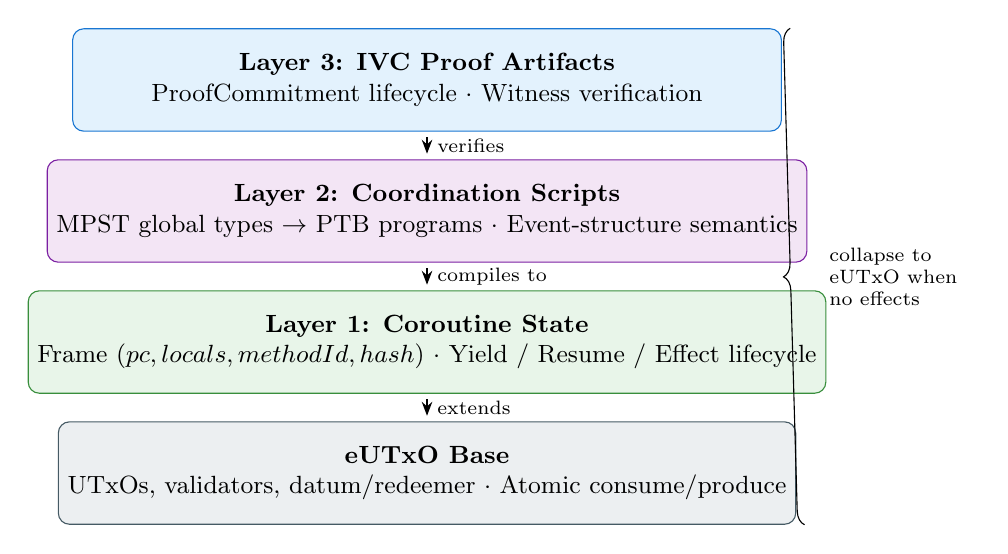
\begin{tikzpicture}[>=Stealth]
%% Nodes
\node[layernode, fill=palBlueLt, draw=palBlue]  (L3) {\textbf{Layer 3: IVC Proof Artifacts}\\ProofCommitment lifecycle $\cdot$ Witness verification};
\node[layernode, fill=palPurpleLt, draw=palPurple, below=0.35cm of L3] (L2) {\textbf{Layer 2: Coordination Scripts}\\MPST global types $\to$ PTB programs $\cdot$ Event-structure semantics};
\node[layernode, fill=palGreenLt, draw=palGreen, below=0.35cm of L2]  (L1) {\textbf{Layer 1: Coroutine State}\\Frame $(pc, locals, methodId, hash)$ $\cdot$ Yield / Resume / Effect lifecycle};
\node[layernode, fill=palGrayLt, draw=palGray, below=0.35cm of L1]   (L0) {\textbf{eUTxO Base}\\UTxOs, validators, datum/redeemer $\cdot$ Atomic consume/produce};
%% Edges
\draw[stdarrow] (L3) -- node[right, font=\scriptsize] {verifies} (L2);
\draw[stdarrow] (L2) -- node[right, font=\scriptsize] {compiles to} (L1);
\draw[stdarrow] (L1) -- node[right, font=\scriptsize] {extends} (L0);
%% Annotation
\draw[decorate, decoration={brace, amplitude=5pt, mirror}]
  ([xshift=3pt]L3.north east) -- ([xshift=3pt]L0.south east)
  node[midway, right=8pt, font=\scriptsize, align=left, text width=1.8cm]
  {collapse to eUTxO when no effects};
\end{tikzpicture}
\end{adjustbox}
\caption{Architecture layers of ICE-UTxO. Layer~1 (coroutine state) extends UTxOs with frames; Layer~2 (coordination) compiles MPST global types to PTB programs; Layer~3 (verification) attaches IVC proof artifacts. When no coroutines yield and no effects are raised, all three layers collapse and ICE-UTxO degenerates to standard eUTxO.}
\label{fig:architecture}
\end{figure}

\subsection{Scope and Non-Goals}\label{sec:scope}

This paper addresses the formal model and mechanized safety proofs. Implementation performance, ZK circuit design, developer tooling, and incentive design are out of scope. Deployment architecture and S-BAC coordination are addressed in a companion paper~\cite{PaperB}.

\subsection{Deployment Model: S-BAC for Cross-Shard Atomicity}\label{sec:deployment}

Owned-object transactions proceed without full consensus; shared-object transactions require S-BAC~\cite{AlBassam2018} for atomic commit:

\begin{itemize}
  \item Each shard checks its \emph{local projection} of the coordination script during the prepare phase.
  \item The IVC witness lets shards validate the interleaving without re-executing private computation.
  \item If all shards prepare successfully, the transaction commits; if any shard aborts, all abort.
\end{itemize}

\begin{table}[t]
\caption{Mapping from Chainspace to ICE-UTxO.}
\label{tab:chainspace-mapping}
\centering
\begin{tabular}{ll}
\toprule
\textbf{Chainspace} & \textbf{ICE-UTxO} \\
\midrule
Object & Frame-carrying UTxO \\
Procedure bundle & PTB program + IVC witness \\
Checker & Witness verifier + ledger checks \\
S-BAC & Cross-shard atomic commit \\
\bottomrule
\end{tabular}
\end{table}

\subsection{Formal Verification}\label{sec:verification-intro}

The ICE-UTxO ledger-level semantics have been formalized in Lean~4 across thirteen source files organized in four core modules (\texttt{StarstreamPilot.lean}, \texttt{Script.lean}, \texttt{PTB.lean}, \texttt{SBAC.lean}), two extension modules (\texttt{ConservativeExtension.lean}, \texttt{OptimisticMode.lean}), and supporting oracle modules. Cryptographic primitives and the S-BAC consensus layer are modeled as oracles with explicit assumptions (\cref{sec:state-components}). Every lemma is fully proved; the development relies only on the standard Lean kernel axioms (\texttt{propext}, \texttt{Quot.sound}, \texttt{funext}) and is mostly constructive, with three localized \texttt{by\_contra} case splits on decidable propositions.

\subsection{Contributions}\label{sec:contributions}

This paper makes the following contributions:

\begin{enumerate}
  \item \textbf{ICE-UTxO model.} A conservative extension of eUTxO with coroutines, algebraic effects, and proof-carrying transactions (\cref{sec:model,sec:opsem}).
  \item \textbf{Coordination scripts.} A formal language for multiparty coordination based on MPST global types with event-structure semantics (\cref{sec:model}).
  \item \textbf{PTB compilation.} Translation from coordination scripts to PTB-style bytecode---adapting Sui's Programmable Transaction Block format~\cite{Blackshear2023}---with explicit dataflow and formal correctness guarantees (\cref{sec:model}).
  \item \textbf{S-BAC integration.} Shard-local verification using projected coordination scripts, composing Chainspace's S-BAC protocol~\cite{AlBassam2018} with session-type witnesses to enable protocol-aware cross-shard atomic commit (\cref{sec:model,sec:bridge}).
  \item \textbf{Lean~4 mechanization.} Complete formal verification with mostly constructive proofs (\cref{sec:mechanization}).
  \item \textbf{Strong serializability proof.} A constructive bubble-sort proof that acyclic full-conflict precedence graphs imply all conflict-respecting permutations produce the same core state (\cref{sec:serializability}).
  \item \textbf{Systematic integration.} A demonstration that coroutines, algebraic effects, MPST, PTB compilation, IVC proofs, and S-BAC compose coherently as a conservative extension of eUTxO, with the combination verified end-to-end. Individual components draw on established techniques (\cref{tab:novelty} in \cref{sec:related}); the contribution is their integration within a single formally verified framework.
\end{enumerate}

\noindent The contributions are formal: we establish the model and prove its safety properties via mechanized proof. Empirical evaluation of proving costs, transaction throughput, and validation latency under realistic workloads is complementary and left to implementation work.

\subsection{How to Read This Paper}\label{sec:howtoread}

This paper serves multiple audiences with different interests. The following guide maps reader backgrounds to relevant sections.

\textbf{For blockchain developers}: \cref{sec:intro,sec:state-components,sec:global-types,sec:projection,sec:lifecycle,sec:commit-rule,sec:concurrency-modes} introduce the model and its operational behavior.

\textbf{For formal methods researchers}: \cref{sec:event-structure-semantics,sec:serializability,sec:bridge} contain the main theoretical contributions. \Cref{sec:mechanization} documents the Lean mechanization.

\textbf{For protocol designers}: \cref{sec:sbac-integration,sec:commit-rule,sec:coordination-witness} describe the deployment architecture and its trust boundaries.

\subsection{Paper Roadmap}\label{sec:roadmap}

\Cref{sec:background} reviews background. \Cref{sec:model} presents the ICE-UTxO model in full. \Cref{sec:opsem} defines the operational semantics and proves ledger safety invariants. \Cref{sec:serializability} establishes strong conflict serializability. \Cref{sec:bridge} bridges the MPST coordination layer to the ledger commit mechanism. \Cref{sec:mechanization} discusses the Lean~4 mechanization. \Cref{sec:related} surveys related work. \Cref{sec:discussion} discusses limitations and future directions. \Cref{sec:conclusion} concludes.

%% ═══════════════════════════════════════════════════════════════════════════
\section{Background}\label{sec:background}

ICE-UTxO combines five ideas: eUTxO (state substrate), multiparty session types (coordination), event structures (partial-order semantics), Programmable Transaction Blocks (deterministic execution), and Sharded Byzantine Atomic Commit (cross-shard consistency).

\subsection{Extended UTxO}\label{sec:eutxo}

The eUTxO model~\cite{Chakravarty2020} augments each UTxO with a typed \emph{datum} and each spending transaction with a \emph{redeemer}. Each validator is a pure deterministic gate $\mathit{validator} : \mathit{Datum} \times \mathit{Redeemer} \times \mathit{TxContext} \to \mathit{Bool}$, enabling parallel validation and formal verification.

Despite these strengths, eUTxO cannot express multi-step atomic protocols within a single transaction. The ``consume to read'' problem (inspecting a datum requires consuming the UTxO) forces contention; the \emph{double satisfaction} problem~\cite{Chakravarty2020} allows outputs to be ``stolen'' across script inputs. Cardano's CIP-31 reference inputs~\cite{CIP31} and related CIPs (inline datums, reference scripts, deployed in the Vasil hard fork) reduce contention but do not enable multi-step atomic coordination. Ergo~\cite{Ergo2019} supports multi-stage contracts via ErgoScript; BitML~\cite{Bartoletti2018} provides a process calculus for Bitcoin smart contracts; Vinogradova and Melkonian~\cite{Vinogradova2024} explore inter-transaction message-passing for eUTxO. ICE-UTxO differs by enabling multi-step atomic protocols \emph{within} a single transaction via coroutines and algebraic effects.

\subsection{Multiparty Session Types}\label{sec:mpst-bg}

Multiparty session types (MPST)~\cite{Honda2016} specify communication protocols among multiple roles. A \emph{global type}~$G$ describes the complete protocol; \emph{projection} extracts a local type $L_r = G \upharpoonright r$ for each role~$r$. The metatheory guarantees communication safety, protocol conformance, and progress (deadlock freedom)~\cite{Bettini2008,Coppo2013,Scalas2016}. The grammar is:
\[
G ::= p \to q : \langle S \rangle . G \mid G_1 + G_2 \mid \mu X . G \mid X \mid \mathbf{end}
\]

In ICE-UTxO, sessions are scoped to a single atomic transaction rather than distributed channels. Each UTxO plays a role; its validator enforces the projected local type. Adversarial deviation is prevented by proof-carrying semantics (\cref{sec:model}). Castellani et al.~\cite{Castellani2023} give MPST an event-structure semantics that captures true concurrency; ICE-UTxO builds directly on this interpretation.

\paragraph{A note on formalism.} ICE-UTxO's coordination scripts (\cref{sec:global-types}) are formalized as labeled event structures with a domain-specific action grammar, not as global type terms. The connection is through Castellani et al.'s event-structure semantics. Projection (\cref{sec:projection}) is a set-theoretic filter on events rather than a syntactic operation on the grammar.

\subsection{Event Structures}\label{sec:event-structures-bg}

Event structures~\cite{Winskel1986} model both causal order and mutual exclusion explicitly, distinguishing genuinely independent operations from causally dependent ones. Formally, an event structure is a triple $(E, \leq, \#)$ where $\leq$ is a partial order (causality) and $\#$ is a symmetric, irreflexive conflict relation, subject to \emph{hereditary conflict}: if $e_1 \mathrel{\#} e_2$ and $e_2 \leq e_3$, then $e_1 \mathrel{\#} e_3$. A \emph{configuration} $C \subseteq E$ is conflict-free and down-closed. An event is \emph{enabled} in $C$ if all predecessors are present and no conflicts exist. A \emph{valid trace} is a sequence whose every prefix forms a configuration.

Castellani et al.~\cite{Castellani2023} interpret MPST global types as event structures, giving MPST a true-concurrency semantics. Any acyclic event structure can be linearized; concurrent events may appear in either order, and if the state-transition function commutes on independent operations (\cref{sec:core-state}), all linearizations produce the same state. This confluence property underlies the serializability results (\cref{sec:serializability}). PTB compilation (\cref{sec:ptb-compilation}) performs exactly this linearization.

\Cref{fig:event-dag} illustrates a small event structure arising from a coordination script. Event~$e_1$ (install a handler) causally precedes both $e_2$ (resume coroutine $U_1$) and $e_3$ (resume coroutine $U_2$). Event~$e_2$ causally precedes $e_4$ (raise an effect), which in turn precedes $e_5$ (handle the effect). The dashed line between $e_3$ and $e_4$ denotes conflict: they cannot both appear in the same configuration. This models a protocol where $U_1$ and $U_2$ cannot both be active simultaneously---the coordinator must choose which coroutine to resume, and the unchosen path is excluded from the execution.

\begin{figure}[t]
\centering
\begin{adjustbox}{max width=\linewidth, center}
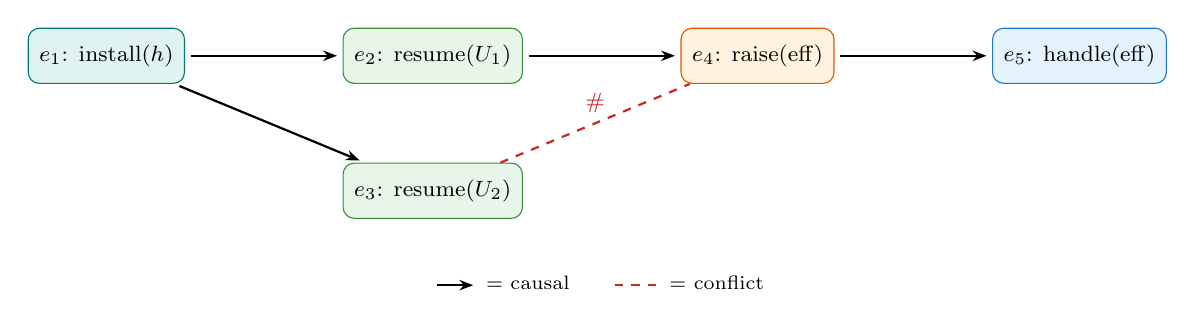
\begin{tikzpicture}[
  node distance=1.5cm and 2.0cm,
  >=Stealth
]
%% Nodes
\node[evtnode, fill=palTealLt, draw=palTeal] (e1) {$e_1$: install$(h)$};
\node[evtnode, fill=palGreenLt, draw=palGreen, right=of e1] (e2) {$e_2$: resume$(U_1)$};
\node[evtnode, fill=palGreenLt, draw=palGreen, below=1.0cm of e2] (e3) {$e_3$: resume$(U_2)$};
\node[evtnode, fill=palOrangeLt, draw=palOrange, right=of e2] (e4) {$e_4$: raise(eff)};
\node[evtnode, fill=palBlueLt, draw=palBlue, right=of e4] (e5) {$e_5$: handle(eff)};
%% Edges
\draw[stdarrow] (e1) -- (e2);
\draw[stdarrow] (e1) -- (e3);
\draw[stdarrow] (e2) -- (e4);
\draw[stdarrow] (e4) -- (e5);
\draw[conflictline] (e3) -- (e4) node[midway, above, font=\footnotesize] {$\#$};
%% Legend — anchored below the entire diagram
\node[font=\scriptsize, anchor=north] at ([yshift=-6mm]current bounding box.south) (leg) {%
  \tikz[baseline=-0.5ex]{\draw[stdarrow](0,0)--(0.6,0);}\;= causal\qquad
  \tikz[baseline=-0.5ex]{\draw[conflictline](0,0)--(0.6,0);}\;= conflict};
\end{tikzpicture}
\end{adjustbox}
\caption{Example event-structure DAG. Solid arrows denote causal order ($<$); the dashed line between $e_3$ and $e_4$ denotes conflict ($\#$).}
\label{fig:event-dag}
\end{figure}

\subsection{Programmable Transaction Blocks}\label{sec:ptb-bg}

\emph{Programmable Transaction Blocks} (PTBs), introduced by Sui~\cite{Blackshear2023}, allow a transaction to contain an ordered sequence of commands $[c_0, \ldots, c_n]$ with explicit dataflow: command $c_i$ stores its result in register $\mathit{Result}(i)$, and subsequent commands reference earlier results as inputs. All commands execute atomically; there are no loops or branches within a PTB. ICE-UTxO adopts the PTB model as a compilation target for its explicit, deterministic schedule. Coordination scripts are compiled to PTB-style programs: the event structure's causal order is linearized into a command sequence with dataflow through result registers. The compilation is formalized in \cref{sec:ptb-compilation}.

\subsection{Sharded Byzantine Atomic Commit (S-BAC)}\label{sec:sbac-bg}

Chainspace~\cite{AlBassam2018} introduced \emph{Sharded Byzantine Atomic Commit} (S-BAC), adapting two-phase commit for Byzantine fault tolerance. In the \emph{prepare} phase, each shard runs BFT consensus to check local validity and locks affected inputs. In the \emph{accept} phase, unanimous prepare votes trigger commit; any abort triggers global abort. Safety holds unconditionally ($f < n/3$ Byzantine validators per shard); liveness requires partial synchrony. ICE-UTxO augments S-BAC with proof-carrying semantics: during prepare, each shard validates its local projection of the coordination script and checks the IVC witness, eliminating the need to re-execute remote computation. The formal integration is detailed in \cref{sec:sbac-integration}.

\medskip
\noindent\textbf{Summary.}
The five foundations provide the state model (eUTxO), protocol specification (MPST with event structures), deterministic execution (PTB), and cross-shard atomicity (S-BAC). ICE-UTxO's central contribution---proof-carrying semantics---is introduced in \cref{sec:model}.

%% ═══════════════════════════════════════════════════════════════════════════
\section{The ICE-UTxO Model}\label{sec:model}

This section presents the formal ICE-UTxO model, built in five steps. First: state components---what the ledger holds (\cref{sec:state-components}). Second: coordination scripts---what interactions are allowed (\cref{sec:global-types}). Third: event-structure semantics---what correctness means (\cref{sec:event-structure-semantics}). Fourth: PTB compilation---how scripts become programs (\cref{sec:ptb-compilation}). Fifth: S-BAC integration---how shards synchronize (\cref{sec:sbac-integration}). Each step answers one question; together they give the complete model.

Readers familiar with eUTxO may focus on \cref{sec:state-components} (Definitions~3.1--3.7) to see what is new in the state model, then skip to \cref{sec:ptb-compilation} for the compilation pipeline. Readers from the session-types community may focus on \cref{sec:global-types,sec:event-structure-semantics,sec:projection} for the event-structure semantics and projection theory.

Standard eUTxO validators execute once and terminate---they cannot pause, request external services, or prove that their coordination with other validators was correct. The state components defined below extend the eUTxO ledger with the machinery needed to support these three capabilities: coroutine suspension (frames), structured service requests (effects and handlers), and cryptographic verification of protocol conformance (proof commitments).

\subsection{State Components}\label{sec:state-components}

Where the standard eUTxO model has only UTxOs and transactions, ICE-UTxO adds five new concepts, introduced in dependency order: \textbf{frames} (coroutine suspension state), \textbf{effects} and \textbf{handlers} (structured service requests and their processors), \textbf{proof commitments} (IVC certificates tracking verification status), and augmented \textbf{transactions} and \textbf{ledger} with effect queues and handler stacks.

We use the following identifier domains, all drawn from $\NN$: $\mathit{UTXOId}$, $\mathit{TxId}$, $\mathit{InterfaceId}$, $\mathit{ProcessId}$, $\mathit{CommitmentHash}$. The formalization does not impose size limits on frames or UTxO datums; in a deployment, maximum frame size would be bounded by transaction size limits, and storage costs would be proportional to frame size.

When a coroutine yields, it serializes its execution state into a \emph{frame} stored as part of the UTxO datum. Resuming reads the frame back and continues from the saved suspension point.

\begin{definition}[Frame]\label{def:frame}
A frame is a tuple $f = (\mathit{pc}, \mathit{locals}, \mathit{methodId}, \mathit{hash})$ where $\mathit{pc} : \NN$ is the program counter (instruction index within the coroutine body), $\mathit{locals} : \text{List}(\mathit{Value})$ stores the coroutine's local variable bindings, $\mathit{methodId} : \NN$ identifies which method or entry point is being executed, and $\mathit{hash} : \mathit{CommitmentHash}$ is a cryptographic commitment chaining this frame to the preceding frame in the coroutine's execution history.
\end{definition}

The $\mathit{hash}$ field chains each frame to its predecessor, ensuring tamper detection. Frame integrity is guaranteed by the IVC proof verification layer (\cref{sec:commit-rule}).

Effects and handlers implement algebraic effects~\cite{PlotkinPretnar2009} at the ledger level: a coroutine raises a structured request and is suspended until a handler fulfills it.

\begin{definition}[Effect]\label{def:effect}
An effect is a triple $e = (\mathit{iface}, \mathit{source}, \mathit{tag})$ where $\mathit{iface} : \mathit{InterfaceId}$ identifies the target interface, $\mathit{source} : \mathit{UTXOId}$ identifies the raising coroutine, and $\mathit{tag} : \NN$ distinguishes effect operations. The three artifacts represent effects at different levels of detail: this paper uses the 3-field triple above; the Lean mechanization adds a fourth field $\mathit{fuel} : \NN$ (a termination measure for effect-subtree recursion); the TLA+ specification uses a 10-field record adding $\mathit{kind}$, $\mathit{continuationId}$, $\mathit{payload}$, $\mathit{handled}$, $\mathit{handlerStackId}$, and $\mathit{witLedgerKind}$ to model dispatch state, IVC witness alignment, and handler-stack bookkeeping. The extra fields do not affect the theorems proved in Lean (which depend only on $\mathit{iface}$, $\mathit{source}$, and $\mathit{tag}$) but are needed for the TLA+ invariants governing handler matching and effect lifecycle.
\end{definition}

Handlers are organized in a LIFO stack per interface; the topmost handler receives dispatched effects.

\begin{definition}[Handler]\label{def:handler}
A handler is a pair $h = (\mathit{iface}, \mathit{hid})$ where $\mathit{iface}$ identifies the interface and $\mathit{hid}$ is a unique handler identifier.
\end{definition}

The final state component is the \emph{proof commitment}. The transaction author generates a cryptographic proof certifying correct execution, attached as a proof commitment that progresses through a lifecycle: $\text{NotStarted} \to \text{Generating} \to \text{Verifying} \to \text{Verified}$ (with failure edges to $\text{Failed}$). Only when all commitments reach $\text{Verified}$ can the transaction commit.

\begin{definition}[Proof Commitment]\label{def:proof-commitment}
A proof commitment records the status of an IVC/PCD (proof-carrying data) proof:
\[
p = (\mathit{proofKind}, \mathit{processId}, \mathit{commitHash}, \mathit{verifyKey}, \mathit{phase}, \mathit{stepNumber})
\]
where $\mathit{proofKind} \in \{\text{IVC\_Step}, \text{IVC\_Accumulator}, \text{Witness}\}$ (the Lean mechanization represents proof kinds as \texttt{Nat}; the enumeration is the intended semantic interpretation) and $\mathit{phase}$ follows:
\[
\text{NotStarted} \to \text{Generating} \to \text{Verifying} \to \text{Verified}
\]
with failure edges from Generating and Verifying to Failed. The $\mathit{commitHash}$ field binds the proof to the transaction context; it is intended to be computed as a hash over the transaction's inputs, outputs, and coordination witness, providing anti-replay protection. The exact hash input is not formalized in the current mechanization (see \cref{sec:commit-rule}, Security Assumption~1).
\end{definition}

\begin{remark}[IVC Proof Predicate]\label{rem:ivc-predicate}
The IVC proof for a transaction with coordination witness $W = (S, \mathit{tr})$ certifies three predicates: (1)~\emph{execution correctness} (each coroutine step produced the correct output frame); (2)~\emph{effect resolution} (every raised effect was dispatched and handled); and (3)~\emph{protocol conformance} ($\mathit{witnessGlobalOK}(W)$: the trace is valid for the script). The $\mathit{commitHash}$ field binds the proof to the transaction context, preventing replay. Soundness rests on Security Assumption~1 (\cref{sec:commit-rule}).
\end{remark}

ICE-UTxO extends the standard eUTxO transaction with $\mathit{readSet}$ (reference inputs), $\mathit{writeSet}$, $\mathit{proofCommitments}$, and $\mathit{phase}$ (lifecycle state).

\begin{definition}[Transaction]\label{def:transaction}
A transaction is:
\[
\mathit{tx} = (\mathit{id}, \mathit{inputs}, \mathit{outputs}, \mathit{readSet}, \mathit{writeSet}, \mathit{proofCommitments}, \mathit{phase})
\]
where $\mathit{inputs}, \mathit{outputs}, \mathit{readSet}, \mathit{writeSet} : \Pfin(\mathit{UTXOId})$, $\mathit{proofCommitments} : \text{List}(\mathit{ProofCommitment})$, and $\mathit{phase} \in \{\text{Idle}, \text{Reserve}, \text{Executing}, \text{Committing}, \text{Committed}, \text{Rollback}, \text{Failed}\}$.
\end{definition}

The ledger state extends the standard UTxO ledger with $\mathit{locked}$, $\mathit{pending}$, $\mathit{effects}$, and $\mathit{handlerStacks}$.

\begin{definition}[Ledger]\label{def:ledger}
The ledger state is:
\[
L = (\mathit{utxos}, \mathit{consumed}, \mathit{locked}, \mathit{pending}, \mathit{history}, \mathit{effects}, \mathit{handlerStacks})
\]
where:
\begin{itemize}
  \item $\mathit{utxos}, \mathit{consumed}, \mathit{locked} : \Pfin(\mathit{UTXOId})$
  \item $\mathit{pending} : \Pfin(\mathit{Tx})$
  \item $\mathit{history} : \text{List}(\mathit{Tx})$ (committed transactions in order)
  \item $\mathit{effects} : \mathit{InterfaceId} \to \text{List}(\mathit{Effect})$ (pending effect queues)
  \item $\mathit{handlerStacks} : \mathit{InterfaceId} \to \text{List}(\mathit{Handler})$ (installed handler stacks)
\end{itemize}
The effects and handler stacks are organized per-interface as stacks, supporting dynamic installation and uninstallation of handlers. When a coroutine raises an effect on interface $i$, it is dispatched to the handler at the top of $\mathit{handlerStacks}(i)$; if the stack is empty, the effect remains unrouted and the transaction must eventually abort or install a replacement handler. Frames are authenticated by the $\mathit{hash}$ field, which chains each frame to its computational history: a resumed coroutine can verify that its frame has not been tampered with by checking the hash against the preceding frame. In a deployment, the hash is checked by the IVC circuit (Layer~3) rather than by the ledger model itself; the formalization treats frame integrity as guaranteed by proof verification (\cref{sec:commit-rule}).
\end{definition}

\begin{table}[t]
\caption{State components of the ICE-UTxO ledger.}
\label{tab:state-components}
\centering\small
\begin{tabular}{lll}
\toprule
\textbf{Component} & \textbf{Type} & \textbf{Purpose} \\
\midrule
$\mathit{utxos}$        & $\Pfin(\mathit{UTXOId})$                              & Currently unspent outputs \\
$\mathit{consumed}$      & $\Pfin(\mathit{UTXOId})$                              & Previously spent outputs (monotonically growing) \\
$\mathit{locked}$        & $\Pfin(\mathit{UTXOId})$                              & Outputs reserved by in-flight transactions \\
$\mathit{pending}$       & $\Pfin(\mathit{Tx})$                                  & Transactions in progress (not yet committed/aborted) \\
$\mathit{history}$       & $\text{List}(\mathit{Tx})$                            & Committed transactions in order \\
$\mathit{effects}$       & $\mathit{InterfaceId} \to \text{List}(\mathit{Effect})$  & Pending service request queues \\
$\mathit{handlerStacks}$ & $\mathit{InterfaceId} \to \text{List}(\mathit{Handler})$ & Installed handler stacks (LIFO per interface) \\
\bottomrule
\end{tabular}
\end{table}

\paragraph{Modeling assumptions.}
The formal model makes several assumptions that should be stated explicitly. Cryptographic hash collision resistance is assumed: the frame hash chaining is secure under standard assumptions. ZK proof verification is treated as a sound oracle: the model does not formalize the internal structure of IVC proofs but assumes that verified proofs correctly attest to computation integrity. Handler dispatch uses top-of-stack semantics; an empty stack means the effect is unroutable. Frame and UTxO datum sizes are bounded by deployment transaction size limits (not formalized). All identifier domains are drawn from $\NN$; the formalization does not enforce type-level distinction between different ID kinds (e.g., $\mathit{UTXOId}$ vs.\ $\mathit{TxId}$); see \cref{sec:discussion} for planned improvements.

\paragraph{Security assumptions.}\label{para:security-assumptions}
The formal guarantees rest on four assumptions, stated here once for auditability. All subsequent safety theorems are conditional on these assumptions; we refer back to this list rather than restating them.
\begin{description}
  \item[SA1 (ZK verifier soundness).] The predicate \texttt{allProofsVerified} is a sound oracle---if it returns true, the attested computation was performed correctly. If this assumption fails, all safety guarantees become vacuous; an adversary can forge proof commitments and commit arbitrary invalid transactions.
  \item[SA2 (Phase discipline).] The transaction executor enforces the phase-transition ordering (Idle $\to$ Reserve $\to$ Executing $\to$ Committing $\to$ Committed). The Lean mechanization proves safety given this ordering; enforcement is a deployment obligation.
  \item[SA3 (S-BAC Byzantine tolerance).] Each shard has at most $f_s < n_s / 3$ Byzantine validators. Under this bound, S-BAC guarantees safety (no invalid commits); a shard exceeding this bound can force aborts of any transaction touching its state, acting as a censorship vector but not violating safety.
  \item[SA4 (Collision-resistant hashing).] The frame hash chain provides computational binding under standard cryptographic assumptions.
\end{description}

The Lean mechanization proves properties of the \emph{abstract model}: ledger-level operational semantics, conflict serializability, MPST projection, and invariant preservation. A concrete deployment must additionally implement ZK verification (SA1), enforce phase discipline (SA2), maintain shard validator honesty below the BFT bound (SA3), and enforce lock timeouts via runtime policy (\cref{sec:liveness}).

\subsection{Coordination Scripts as Global Types}\label{sec:global-types}

ICE-UTxO makes coordination protocols explicit using \emph{coordination scripts} based on MPST global types~\cite{Honda2016}. Each participant has a \emph{role} with a \emph{kind}: $\text{utxo}$ (on-chain UTxO actors), $\text{iface}$ (off-chain services), or $\text{shard}$ (coordinators managing handler lifecycle). The role-kind system enforces a permission discipline (\cref{tab:permissions}).

A script with an empty event set is trivially well-formed, corresponding to a standard eUTxO transaction requiring no coordination (\cref{sec:reduction}).

The three definitions below formalize role kinds, actions, and scripts. A concrete example (\cref{fig:script-example}) follows immediately, walking through a liquidation protocol line by line.

\begin{definition}[Role Kind]\label{def:role-kind}
$\mathit{RoleKind} ::= \text{utxo} \mid \text{iface} \mid \text{shard}$.
\end{definition}

\begin{definition}[Action]\label{def:action}
The action grammar labels events in a coordination script:
\begin{align*}
\mathit{Action} ::=\; & r_1 \to r_2 : \texttt{raise}(i, \mathit{tag}) \\
\mid\; & r_1 \to r_2 : \texttt{resume}(i, \mathit{tag}) \\
\mid\; & r_1 \to r_2 : \texttt{install}(h) \\
\mid\; & r_1 \to r_2 : \texttt{uninstall}(i) \\
\mid\; & r : \texttt{read}(u) \mid r : \texttt{consume}(u) \mid r : \texttt{produce}(u) \\
\mid\; & r : \texttt{lock}(u) \mid r : \texttt{snapshot}(u)
\end{align*}
Actions are either \emph{communication actions} (with sender $r_1$ and receiver $r_2$) for raise/resume/install/uninstall, or \emph{local actions} for UTxO operations performed by a single role. \emph{(Mechanized: \texttt{inductive Action} in Script.lean; accessor functions for UTxO access, interface usage, and role participation are extended in PTB.lean.)}
\end{definition}

\begin{definition}[Script]\label{def:script}
A script is a tuple $S = (\mathit{roles}, \mathit{roleKind}, E, \mathit{lab}, {<}, {\#})$ where $\mathit{roles} : \Pfin(\mathit{RoleId})$, $\mathit{roleKind} : \mathit{RoleId} \to \mathit{RoleKind}$, $E : \Pfin(\mathit{EventId})$, $\mathit{lab} : \mathit{EventId} \to \mathit{Action}$, ${<} \subseteq E \times E$ is an acyclic relation (the causal ordering; the Lean mechanization enforces acyclicity but not transitivity), and ${\#} \subseteq E \times E$ is a symmetric, irreflexive conflict relation.
\end{definition}

\begin{figure}[t]
\centering
\begin{lstlisting}[language={},frame=single,basicstyle=\ttfamily\small]
script LiquidationProtocol {
  roles: oracle: iface, borrower: utxo,
         liquidator: utxo, coordinator: shard;
  events:
    e1: coordinator -> oracle : install(priceHandler);
    e2: borrower -> oracle : raise(getPrice, ETH_USD);
    e3: oracle -> borrower : resume(priceResult, 1500);
    e4: borrower : consume(collateralUtxo);
    e5: liquidator : produce(liquidatedUtxo);
    e6: coordinator -> oracle : uninstall(priceHandler);
  constraints:
    e1 < e2; e2 < e3; e3 < e4; e4 < e5;
    e5 < e6; e1 < e6;
}
\end{lstlisting}
\caption{Example coordination script with action grammar.}
\label{fig:script-example}
\end{figure}

To make the script notation concrete, consider \cref{fig:script-example} line by line. The script declares four roles: \texttt{oracle} (an interface role representing a price feed service), \texttt{borrower} and \texttt{liquidator} (UTxO roles representing on-chain participants), and \texttt{coordinator} (a shard role managing handler lifecycle). Event $e_1$ installs a price handler on the oracle interface---this must happen before any price queries. Event $e_2$ has the borrower raise a \texttt{getPrice} effect, requesting the current ETH/USD price from the oracle. Event $e_3$ has the oracle resume the borrower with the price result. Events $e_4$ and $e_5$ perform the actual liquidation: the borrower consumes the collateral UTxO and the liquidator produces a new UTxO with the liquidated assets. Finally, $e_6$ uninstalls the price handler. The constraints encode the causal ordering: the handler must be installed before any price query ($e_1 < e_2$), the query must complete before the result is available ($e_2 < e_3$), the result must be known before liquidation proceeds ($e_3 < e_4 < e_5$), and the handler must remain installed until after liquidation ($e_5 < e_6$, $e_1 < e_6$).

\begin{definition}[Well-Formedness]\label{def:well-formedness}
A script $S$ is \emph{well-formed}, written $\mathit{WF}(S)$, if all of the following hold:
\begin{enumerate}
  \item \textbf{orderDom}: both endpoints of every edge in ${<}$ are in $E$.
  \item \textbf{orderAcyclic}: ${<}$ is acyclic (and therefore irreflexive).
  \item \textbf{conflictDom}: both endpoints of every edge in ${\#}$ are in $E$.
  \item \textbf{conflictIrrefl}: ${\#}$ is irreflexive ($\neg(e \mathbin{\#} e)$ for all $e$).
  \item \textbf{conflictSymm}: ${\#}$ is symmetric ($e_1 \mathbin{\#} e_2 \implies e_2 \mathbin{\#} e_1$).
  \item \textbf{rolesOK}: all roles referenced in event labels are declared in $\mathit{roles}$.
  \item \textbf{roleKindOK}: UTxO operations ($\texttt{read}$, $\texttt{consume}$, etc.) are performed only by roles of kind $\text{utxo}$. The Lean mechanization enforces this restriction; the $\text{iface}$ and $\text{shard}$ restrictions shown in \cref{tab:permissions} are design-level constraints that are not yet formalized (the Lean predicate returns $\mathit{True}$ for all non-UTxO actions).
\end{enumerate}
In the Lean formalization, well-formedness is a conjunction of these seven predicates, all defined in \texttt{Script.lean}.
\end{definition}

\paragraph{Formalization gap: incomplete permission enforcement.}
The Lean predicate \texttt{roleKindOK} enforces only the UTxO restriction; the catch-all branch returns $\mathit{True}$ for non-UTxO actions. The $\text{iface}$ and $\text{shard}$ restrictions in \cref{tab:permissions} are design-level constraints not yet formalized. No theorem exploits the missing branches, so all verified results remain sound.

\begin{remark}[Hereditary conflict]\label{rem:hereditary-conflict}
Winskel's original event structures require hereditary conflict: $e_1 \mathbin{\#} e_2 \wedge e_2 < e_3 \implies e_1 \mathbin{\#} e_3$. Our well-formedness conditions omit this. No theorem depends on it; PTB-compiled scripts satisfy it by construction. Adding it as an eighth condition is planned (\cref{sec:discussion}).
\end{remark}

\subsection{Event-Structure Semantics}\label{sec:event-structure-semantics}

The following definitions formalize configurations, enablement, and valid traces for coordination scripts. All are mechanized in \texttt{Script.lean}.

\begin{definition}[Configuration]\label{def:configuration}
A set $C \subseteq E$ is a \emph{configuration} of script $S$ if $C \subseteq S.\mathit{events}$, $C$ is conflict-free, and $C$ is down-closed.
\end{definition}

\begin{definition}[Enablement]\label{def:enablement}
Event $e$ is \emph{enabled} in configuration $C$ if $e \in S.\mathit{events}$, $e \notin C$, all predecessors are in $C$, and $e$ does not conflict with any event in $C$.
\end{definition}

\begin{definition}[Valid Trace]\label{def:valid-trace}
A \emph{valid trace} is a sequence $[e_1, \ldots, e_n]$ admitting a chain $\emptyset = C_0 \to C_1 \to \cdots \to C_n$ of configurations where each $e_i$ is enabled in $C_{i-1}$.
\end{definition}

These definitions are replicated for local scripts (\texttt{LocalScript}) with identical structure; the same semantic framework applies at both global and local levels.

\subsection{Projection and Local Conformance}\label{sec:projection}

Projection extracts from a global script the events relevant to a single role. The projected local script is well-formed (\cref{thm:proj-wf}), enabling shard-local verification: global correctness decomposes into local correctness (\cref{thm:proj-traces,cor:global-implies-local}) and reconstructs from it (\cref{thm:consistent-implies-global}).

\begin{table}[h]
\caption{Permission matrix for role kinds. Only the \texttt{utxo} row is mechanically enforced in Lean; the \texttt{iface} and \texttt{shard} restrictions are design constraints.}
\label{tab:permissions}
\centering\small
\begin{tabular}{lccc}
\toprule
\textbf{Action} & \texttt{utxo} & \texttt{iface} & \texttt{shard} \\
\midrule
\texttt{read}, \texttt{consume}, \texttt{produce}, \texttt{lock}, \texttt{snapshot} & yes$^\dagger$ & no$^\dagger$ & no$^\dagger$ \\
\texttt{raise} (sender) & yes$^\dagger$ & no$^\dagger$ & no$^\dagger$ \\
\texttt{resume} (sender) & no & yes & no \\
\texttt{install}, \texttt{uninstall} (sender) & no & no & yes \\
Any action (receiver) & yes & yes & yes \\
\bottomrule
\end{tabular}

\smallskip\noindent{\footnotesize $^\dagger$Mechanically verified in Lean. All other restrictions are design-level and not yet formalized.}
\end{table}

\noindent Formally, define $\mathit{permitted}(k, a)$ as:
\[
\mathit{permitted}(k, a) \iff \begin{cases}
k = \text{utxo} & \text{if } a \in \{\texttt{read}, \texttt{consume}, \texttt{produce}, \texttt{lock}, \texttt{snapshot}, \texttt{raise}\text{ (sender)}\} \\
k = \text{iface} & \text{if } a = \texttt{resume}\text{ (sender)} \\
k = \text{shard} & \text{if } a \in \{\texttt{install}, \texttt{uninstall}\}\text{ (sender)} \\
\mathit{true} & \text{if } a\text{ is a receiver action}
\end{cases}
\]
The \textbf{WF-RoleKind} predicate (\cref{def:well-formedness}) requires $\mathit{permitted}(\mathit{roleKind}(r), a)$ for every event whose sender is $r$ with action $a$.

\begin{definition}[Participation]\label{def:participation}
Role $r$ \emph{participates} in event $e$ if $r$ appears as sender or receiver in $\mathit{lab}(e)$, or $\mathit{lab}(e)$ is a UTxO action performed by $r$. Formally, $r \in \mathit{participants}(\mathit{lab}(e))$.
\end{definition}

\begin{definition}[Relevance]\label{def:relevance}
Event $e$ is \emph{relevant} to role $r$, written $\mathit{relevant}(r, e)$, if $\mathit{toLocal}(r, \mathit{lab}(e)) \neq \text{None}$, where $\mathit{toLocal}$ converts a global action to a local action from $r$'s perspective:
\begin{itemize}
  \item $r_1 \to r_2 : \texttt{raise}(i, t)$ becomes $\texttt{outRaise}(r_2, i, t)$ if $r = r_1$, or $\texttt{inRaise}(r_1, i, t)$ if $r = r_2$.
  \item UTxO actions become local variants (e.g., $r : \texttt{read}(u)$ becomes $\texttt{localRead}(u)$).
  \item Otherwise $\text{None}$.
\end{itemize}
\end{definition}

\begin{definition}[Projection]\label{def:projection}
Given script $S$ and role $r$, the projection $\mathit{Proj}(S, r)$ is the local script $(E_r, \mathit{lab}_r, {<_r}, {\#_r})$ where $E_r = \{e \in E \mid \mathit{relevant}(r, e)\}$ and the relations are restricted to $E_r \times E_r$.
\end{definition}

\begin{figure}[t]
\centering
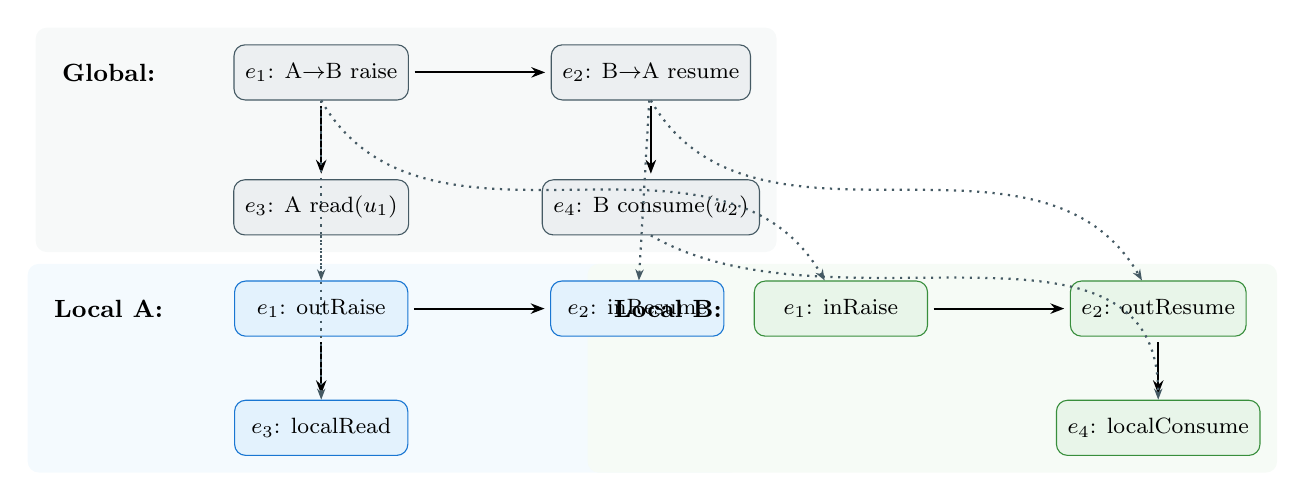
\begin{tikzpicture}[
  node distance=1.0cm and 1.8cm,
  pevt/.style={evtnode, minimum width=2.2cm},
  >=Stealth
]
\def\xLabel{-1.5}   % x-position for section labels
\def\xFirst{1.2}    % x-position for first event column
\def\yGlobal{2.5}   % y-position for Global row
\def\yLocalA{-0.5}  % y-position for Local A row
\def\xLocalBFirst{7.8} % x-position for Local B first event

%% Global Nodes
\node[font=\small\bfseries] (glabel) at (\xLabel, \yGlobal) {Global:};
\node[pevt, fill=palGrayLt, draw=palGray] (g1) at (\xFirst, \yGlobal) {$e_1$: A$\to$B raise};
\node[pevt, fill=palGrayLt, draw=palGray, right=of g1] (g2) {$e_2$: B$\to$A resume};
\node[pevt, fill=palGrayLt, draw=palGray, below=of g1] (g3) {$e_3$: A read($u_1$)};
\node[pevt, fill=palGrayLt, draw=palGray, below=of g2] (g4) {$e_4$: B consume($u_2$)};
\draw[stdarrow] (g1) -- (g2);
\draw[stdarrow] (g1) -- (g3);
\draw[stdarrow] (g2) -- (g4);

%% Local A Nodes
\node[font=\small\bfseries] (alabel) at (\xLabel, \yLocalA) {Local A:};
\node[pevt, fill=palBlueLt, draw=palBlue] (a1) at (\xFirst, \yLocalA) {$e_1$: outRaise};
\node[pevt, fill=palBlueLt, draw=palBlue, right=of a1] (a2) {$e_2$: inResume};
\node[pevt, fill=palBlueLt, draw=palBlue, below=0.8cm of a1] (a3) {$e_3$: localRead};
\draw[stdarrow] (a1) -- (a2);
\draw[stdarrow] (a1) -- (a3);

%% Local B Nodes
\node[pevt, fill=palGreenLt, draw=palGreen] (b1) at (\xLocalBFirst, \yLocalA) {$e_1$: inRaise};
\node[font=\small\bfseries, anchor=east] (blabel) at ([xshift=-8pt]b1.west) {Local B:};
\node[pevt, fill=palGreenLt, draw=palGreen, right=of b1] (b2) {$e_2$: outResume};
\node[pevt, fill=palGreenLt, draw=palGreen, below=0.8cm of b2] (b4) {$e_4$: localConsume};
\draw[stdarrow] (b1) -- (b2);
\draw[stdarrow] (b2) -- (b4);

%% Backgrounds
\begin{scope}[on background layer]
  \node[rounded corners, fill=palGrayLt!40, fit=(glabel)(g1)(g2)(g3)(g4), inner sep=6pt] {};
  \node[rounded corners, fill=palBlueLt!40, fit=(alabel)(a1)(a2)(a3), inner sep=6pt] {};
  \node[rounded corners, fill=palGreenLt!40, fit=(blabel)(b1)(b2)(b4), inner sep=6pt] {};
\end{scope}

%% Projection Arrows
\draw[stutterarrow, palGray] (g1) -- (a1);
\draw[stutterarrow, palGray] (g2) -- (a2);
\draw[stutterarrow, palGray] (g3) -- (a3);
\draw[stutterarrow, palGray] (g1.south) to[out=-60, in=120] (b1);
\draw[stutterarrow, palGray] (g2.south) to[out=-60, in=120] (b2);
\draw[stutterarrow, palGray] (g4.south) to[out=-30, in=90] (b4);
\end{tikzpicture}
\caption{Projection: a global script decomposes into local scripts for each role.}
\label{fig:projection}
\end{figure}

\begin{definition}[Trace Projection]\label{def:trace-projection}
$\mathit{traceProj}(S, r, \mathit{tr}) = \mathit{tr}.\texttt{filter}(\mathit{relevant}(r, \cdot))$.
\end{definition}

\begin{definition}[Local Conformance]\label{def:local-conformance}
Script $S$ \emph{locally conforms} for role $r$ on trace $\mathit{tr}$, written $\mathit{localConform}(S, r, \mathit{tr})$, if $\mathit{Proj}(S, r)$ is well-formed and $\mathit{tr}$ is a valid trace of $\mathit{Proj}(S, r)$.
\end{definition}

\begin{theorem}[Projection Preserves Well-Formedness]\label{thm:proj-wf}
If $\mathit{WF}(S)$ then $\mathit{WF}(\mathit{Proj}(S, r))$ for all roles $r$. \emph{(Mechanized: \texttt{project\_wellFormed}, Script.lean.)}
\end{theorem}

\begin{theorem}[Projection Preserves Traces]\label{thm:proj-traces}
If $\mathit{tr}$ is a valid trace of $S$, then $\mathit{traceProj}(S, r, \mathit{tr})$ is a valid trace of $\mathit{Proj}(S, r)$. \emph{(Mechanized: \texttt{proj\_validTrace}, Script.lean.)}
\end{theorem}

\begin{corollary}[Global Conformance Implies Local]\label{cor:global-implies-local}
If $S$ globally conforms on trace $\mathit{tr}$, then $S$ locally conforms for every role $r$ on $\mathit{traceProj}(S, r, \mathit{tr})$. \emph{(Mechanized: \texttt{proj\_localConform\_of\_globalConform}, Script.lean.)}
\end{corollary}

\subsection{PTB Compilation}\label{sec:ptb-compilation}

A coordination script's event structure admits many valid linearizations---any topological sort of the causal DAG respects the acyclic order. On-chain validators, however, need a single concrete command sequence to replay and verify. PTB compilation selects one such linearization and encodes it as a Programmable Transaction Block (PTB), inspired by Sui's transaction format~\cite{Blackshear2023}: a sequence of commands where each command produces a result stored in a numbered register $\mathit{Result}(i)$, and later commands reference earlier results as inputs, creating an explicit dataflow graph.

The property that matters is determinism. The event structure captures what \emph{could} happen; the PTB captures what \emph{did} happen. Determinism makes on-chain validation possible: validators replay the exact command sequence and verify that the result matches the proof. The correctness criterion is that the PTB's induced event structure (derived from its dependency and conflict relations) is well-formed and admits the PTB's command sequence as a valid trace (Theorems~\ref{thm:toscript-wf}--\ref{thm:valid-trace-trace}). A concrete worked example appears in \cref{sec:worked-example}; the formal definitions follow. All definitions and theorems are mechanized in \texttt{PTB.lean}.

\subsubsection{Command Model}\label{sec:command-model}

\begin{definition}[Command]\label{def:command}
A command is a triple $c = (\mathit{action}, \mathit{uses}, \mathit{conflicts})$ where $\mathit{action} : \mathit{Action}$, $\mathit{uses} : \Pfin(\NN)$ identifies result registers consumed as inputs, and $\mathit{conflicts} : \Pfin(\NN)$ records explicit conflict edges.
\end{definition}

\begin{definition}[Program]\label{def:program}
A PTB program is a list of commands $P = [c_0, \ldots, c_{n-1}]$. Command $c_i$ stores its output in register $\mathit{Result}(i)$, and may reference $\mathit{Result}(j)$ for $j \in c_i.\mathit{uses}$. Well-formedness requires $j < i$ for every $j \in c_i.\mathit{uses}$.
\end{definition}

\begin{definition}[Config]\label{def:config}
A PTB configuration $(\mathit{roles}, \mathit{roleKind})$ maps identifiers to roles and roles to kinds, connecting the PTB to the coordination layer's role structure. (In the Lean mechanization, this corresponds to \texttt{structure Config} in PTB.lean; an extended variant \texttt{AccessConfig} adds $\mathit{utxoRole}$ and $\mathit{ifaceRole}$ mappings used by the witness construction theorems.)
\end{definition}

\subsubsection{Derived Relations}\label{sec:derived-relations}

Given a program $P$, we derive three dependency relations ($\mathit{dataDep}$, $\mathit{utxoDep}$, $\mathit{handlerDep}$) that contribute to the causal order, plus one conflict marker ($\mathit{explicitConflict}$) for choice branches, and combine these into two structural relations: $\mathit{orderRel}$ (causal order) and $\mathit{conflictRel}$ (mutual exclusion). Each action~$a$ exposes accessor functions: $a.\mathit{readUtxos}$, $a.\mathit{writeUtxos}$, $a.\mathit{consumedUtxos}$, $a.\mathit{ifaceUses}$, $a.\mathit{ifaceInstalls}$, $a.\mathit{ifaceUninstalls}$.

\begin{definition}[Dependencies]\label{def:dependencies}
For commands $c_i, c_j$ with $i < j$:
\begin{itemize}
  \item $\mathit{dataDep}(i, j) \iff i \in c_j.\mathit{uses}$ --- result register dependency.
  \item $\mathit{utxoDep}(i, j) \iff c_i.\mathit{writeUtxos} \cap c_j.\mathit{utxoAccesses} \neq \emptyset \;\lor\; c_j.\mathit{writeUtxos} \cap c_i.\mathit{utxoAccesses} \neq \emptyset$ --- read-write or write-write overlap.
  \item $\mathit{handlerDep}(i, j) \iff c_i.\mathit{ifaceInstalls} \cap c_j.\mathit{ifaceUses} \neq \emptyset \;\lor\; c_i.\mathit{ifaceUses} \cap c_j.\mathit{ifaceUninstalls} \neq \emptyset$ --- install-before-use or use-before-uninstall.
\end{itemize}
\end{definition}

\begin{definition}[Order Relation]\label{def:order-rel}
$\mathit{orderRel}(i, j) \iff i < |P| \wedge j < |P| \wedge i < j \wedge (\mathit{dataDep}(i,j) \lor \mathit{utxoDep}(i,j) \lor \mathit{handlerDep}(i,j))$.
\end{definition}

\begin{definition}[Conflict Relation]\label{def:conflict-rel}
$\mathit{conflictRel}(i, j) \iff i < |P| \wedge j < |P| \wedge i \neq j \wedge (c_i.\mathit{consumedUtxos} \cap c_j.\mathit{consumedUtxos} \neq \emptyset \lor c_i.\mathit{ifaceInstalls} \cap c_j.\mathit{ifaceInstalls} \neq \emptyset \lor \mathit{explicitConflict}(i, j))$.
\end{definition}

\begin{remark}[Hereditary Conflict]\label{rem:conflict-properties}
The relation $\mathit{conflictRel}$ is symmetric (by commutativity of set intersection and the $i \neq j$ guard) and irreflexive (since $i \neq j$ is required), but does \emph{not} enforce hereditary conflict (downward closure of conflict under causality), as required by Winskel's original event structures~\cite{Winskel1986}. In Winskel's formulation, if $e \mathrel{\#} e'$ and $e' \leq e''$, then $e \mathrel{\#} e''$: conflict propagates forward through causality. ICE-UTxO omits this because: (i)~PTB-derived event structures have finite, acyclic order relations where the precedence graph's acyclicity check (\cref{def:ledger-invariant}, component~6) is sufficient for serializability without hereditary closure; (ii)~the serializability proof (\cref{thm:strong-serial}) depends on $\mathit{fullConflicts}$ symmetry and $\mathit{CoreState}$ commutativity, not on hereditary propagation; and (iii)~the projection theorems (\cref{thm:proj-wf,thm:proj-traces}) hold for the weaker conflict relation. Adding hereditary closure would strengthen the specification against modeling errors in hand-written scripts (where causal chains might introduce implicit conflicts) and is planned (\cref{sec:discussion}). For PTB-compiled scripts, the omission has no effect on the mechanized results: the $\mathit{toScript}$ translation produces conflict edges only between commands at the same causal depth, so hereditary closure would add no new edges.
\end{remark}

\subsubsection{Translation to Event Structure}\label{sec:translation}

\begin{definition}[toScript]\label{def:toscript}
Given configuration $\mathit{cfg}$ and program $P$, the induced script is:
\[
\mathit{toScript}(\mathit{cfg}, P) = (\mathit{cfg}.\mathit{roles}, \mathit{cfg}.\mathit{roleKind}, \{0, \ldots, |P|-1\}, \lambda i.\, c_i.\mathit{action}, \mathit{orderRel}, \mathit{conflictRel})
\]
\end{definition}

\begin{remark}[Compilation Direction]\label{rem:compilation-direction}
The translation is from programs to event structures, not the reverse. The PTB program specifies \emph{what to execute}; the event structure extracted by $\mathit{toScript}$ specifies \emph{what constraints must hold}. A reverse direction would require solving a scheduling problem and is unnecessary: transaction authors construct PTB programs directly, and the ledger verifies the induced event structure.
\end{remark}

\begin{theorem}[toScript Well-Formedness]\label{thm:toscript-wf}
If $P$ satisfies $\mathit{rolesOK}$ and $\mathit{roleKindOK}$ with respect to $\mathit{cfg}$, then $\mathit{toScript}(\mathit{cfg}, P)$ is well-formed. \emph{(Mechanized: \texttt{Program.toScript\_wellFormed}, PTB.lean.)}
\end{theorem}

\begin{proof}[Proof sketch]
The seven well-formedness predicates decompose as follows. \textbf{WF-Order} and \textbf{WF-Conflict}: both endpoints are in $\{0, \ldots, |P|-1\}$ by the bound guards in the relation definitions. \textbf{WF-Irrefl} and \textbf{WF-Symm} for conflict: irreflexivity follows from $i \neq j$; symmetry from \texttt{conflictRel\_symm}. \textbf{WF-Acyclic}: if $\mathit{orderRel}^+(i, i)$ held, then $i < i$ by transitivity of the $i < j$ constraint in each order edge---contradiction. \textbf{WF-Roles} and \textbf{WF-RoleKind}: by hypothesis.
\end{proof}

\subsubsection{Valid Traces and Witness Construction}\label{sec:valid-traces}

\begin{figure}[t]
\centering
\begin{adjustbox}{max width=\linewidth, center}
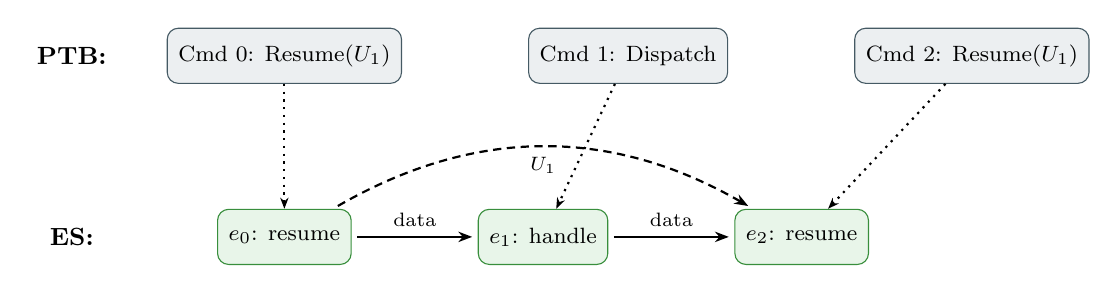
\begin{tikzpicture}[
  node distance=0.8cm and 1.6cm,
  >=Stealth
]
\def\xLabel{-1.2}  % x-position for row labels
\def\xFirst{1.5}   % x-position for first command/event
\def\yPTB{1.8}     % y-position for PTB row
\def\yES{-0.5}     % y-position for ES row

%% PTB Row
\node[font=\small\bfseries] at (\xLabel, \yPTB) {PTB:};
\node[evtnode, fill=palGrayLt, draw=palGray] (c0) at (\xFirst, \yPTB) {Cmd 0: Resume($U_1$)};
\node[evtnode, fill=palGrayLt, draw=palGray, right=of c0] (c1) {Cmd 1: Dispatch};
\node[evtnode, fill=palGrayLt, draw=palGray, right=of c1] (c2) {Cmd 2: Resume($U_1$)};

%% ES Row
\node[font=\small\bfseries] at (\xLabel, \yES) {ES:};
\node[evtnode, fill=palGreenLt, draw=palGreen] (e0) at (\xFirst, \yES) {$e_0$: resume};
\node[evtnode, fill=palGreenLt, draw=palGreen, right=of e0] (e1) {$e_1$: handle};
\node[evtnode, fill=palGreenLt, draw=palGreen, right=of e1] (e2) {$e_2$: resume};

%% Data Edges
\draw[stdarrow] (e0) -- node[above, font=\scriptsize] {data} (e1);
\draw[stdarrow] (e1) -- node[above, font=\scriptsize] {data} (e2);
\draw[stdarrow, densely dashed, bend left=30] (e0) to node[below, font=\scriptsize] {$U_1$} (e2);

%% Mapping Arrows
\draw[stutterarrow] (c0) -- (e0);
\draw[stutterarrow] (c1) -- (e1);
\draw[stutterarrow] (c2) -- (e2);
\end{tikzpicture}
\end{adjustbox}
\caption{PTB compilation mapping commands to event structures.}
\label{fig:ptb-compilation}
\end{figure}

\begin{theorem}[validTrace\_trace]\label{thm:valid-trace-trace}
If $P$ has no conflicts, then the full program-order trace $[0, \ldots, |P|-1]$ is a valid trace of $\mathit{toScript}(\mathit{cfg}, P)$. \emph{(Mechanized: \texttt{Program.validTrace\_trace}, PTB.lean.)}
\end{theorem}

\begin{theorem}[witnessGlobalOK\_of]\label{thm:witness-global-ok}
If $P$ satisfies $\mathit{rolesOK}$, $\mathit{roleKindOK}$, $\mathit{conflictFree}(\mathit{keep})$, and $\mathit{downClosed}(\mathit{keep})$, then $\mathit{toWitness}(\mathit{cfg}, P, \mathit{keep})$ is globally OK. \emph{(Mechanized: \texttt{Program.witnessGlobalOK\_of}, PTB.lean.)}
\end{theorem}

\begin{theorem}[validTrace\_traceOf]\label{thm:valid-trace-traceof}
Given a predicate $\mathit{keep} : \NN \to \mathit{Bool}$ such that $P$ is conflict-free on $\mathit{keep}$ and $\mathit{keep}$ is down-closed with respect to $\mathit{orderRel}$, the filtered trace $P.\mathit{traceOf}(\mathit{keep})$ is a valid trace of $\mathit{toScript}(\mathit{cfg}, P)$. \emph{(Mechanized: \texttt{Program.validTrace\_traceOf}, PTB.lean.)}
\end{theorem}

\begin{theorem}[crossRoleSafe\_of\_access]\label{thm:cross-role-safe}
If every command's access roles are contained in its participant set ($\mathit{accessRolesOK}$) and explicit conflicts are shared ($\mathit{explicitConflictShared}$), then conflicting commands always share at least one role. \emph{(Mechanized: \texttt{Program.crossRoleSafe\_of\_access}, PTB.lean.)}
\end{theorem}

\paragraph{Choice and the \texttt{keep} predicate.} The predicate $\mathit{keep} : \NN \to \mathit{Bool}$ selects which commands are executed, modeling branching. For linear protocols, $\mathit{keep} = \lambda i.\, \mathit{true}$; for exclusive choices via $\mathit{conflictRel}(i, j)$, exactly one is kept. The conditions---conflict-free and down-closed---ensure the selected subset is a valid configuration (\cref{def:configuration}). The transaction author constructs $\mathit{keep}$ during execution and includes it in the coordination witness; the IVC proof certifies correctness by binding $\mathit{keep}$ into the $\mathit{commitHash}$.

\subsubsection{Worked Example}\label{sec:worked-example}

Consider the collateralized loan scenario from \cref{sec:problem}, compiled to a 3-command PTB:

\begin{table}[h]
\centering\small
\begin{tabular}{cllcc}
\toprule
$i$ & \textbf{Command} & \textbf{Action} & \textbf{uses} & \textbf{conflicts} \\
\midrule
0 & Resume borrower coroutine & $\texttt{resume}(r_b, r_o, \mathit{oracle}, \mathit{getPrice})$ & $\emptyset$ & $\emptyset$ \\
1 & Dispatch to price handler & $\texttt{raise}(r_o, r_h, \mathit{oracle}, \mathit{dispatch})$ & $\{0\}$ & $\emptyset$ \\
2 & Resume with price result & $\texttt{resume}(r_h, r_b, \mathit{oracle}, \mathit{result})$ & $\{1\}$ & $\emptyset$ \\
\bottomrule
\end{tabular}
\end{table}

\paragraph{Derived edges.} $\mathit{dataDep}(0,1)$ since $0 \in c_1.\mathit{uses}$; $\mathit{dataDep}(1,2)$ since $1 \in c_2.\mathit{uses}$; $\mathit{handlerDep}(0,2)$ since both access the oracle interface. Thus $\mathit{orderRel} = \{(0,1), (1,2), (0,2)\}$ and $\mathit{conflictRel} = \emptyset$.

\paragraph{Induced script.} $\mathit{toScript}$ produces events $\{0,1,2\}$ with order $0 < 1 < 2$ (plus $0 < 2$) and no conflict. This is a total order, so the unique valid trace is $[0,1,2]$.

\paragraph{Validity.} Since $\mathit{conflictRel} = \emptyset$, \cref{thm:valid-trace-trace} applies directly: the program-order trace $[0,1,2]$ is valid. By \cref{thm:witness-global-ok}, $\mathit{toWitness}(\mathit{cfg}, P, \lambda i.\, \mathit{true})$ is globally OK.

\paragraph{Witness and verification.} The valid trace $[0, 1, 2]$ is packaged into the coordination witness $W = (S, [0, 1, 2])$, which the IVC proof certifies (\cref{rem:ivc-predicate}). Under S-BAC (\cref{sec:sbac-integration}), each shard checks only its roles' projected trace and UTxO liveness; the bidirectional witness theorems (\cref{thm:global-implies-local,thm:consistent-implies-global}) ensure this suffices for the global guarantee.

\subsection{S-BAC Integration}\label{sec:sbac-integration}

When a transaction spans multiple shards, S-BAC~\cite{AlBassam2018} ensures all-or-nothing commit. ICE-UTxO improves over Chainspace by having shards check local trace conformance and UTxO liveness rather than re-executing transaction logic; the IVC proof certifies the rest.

\begin{definition}[S-BAC Configuration]\label{def:sbac-config}
An S-BAC configuration is a pair $(\mathit{shardOfUtxo}, \mathit{rolesOfShard})$ mapping UTxOs to shards and shards to their associated roles.
\end{definition}

\begin{definition}[Coordination Witness]\label{def:coord-witness}
A coordination witness is a pair $W = (S, \mathit{tr})$ of a script $S$ and a trace $\mathit{tr}$.
\end{definition}

\begin{definition}[Witness Predicates]\label{def:witness-predicates}
\begin{align*}
\mathit{witnessGlobalOK}(W) &\iff S.\mathit{globalConform}(\mathit{tr}) \\
\mathit{witnessLocalOK}(W) &\iff \forall r \in S.\mathit{roles}.\; S.\mathit{localConform}(r, S.\mathit{traceProj}(r, \mathit{tr})) \\
\mathit{witnessConsistent}(W) &\iff S.\mathit{traceConsistent}(\mathit{tr})
\end{align*}
\end{definition}

\begin{theorem}[Global Implies Local]\label{thm:global-implies-local}
$\mathit{witnessGlobalOK}(W) \implies \mathit{witnessLocalOK}(W)$. \emph{(Mechanized: \texttt{witnessLocalOK\_of\_global}, SBAC.lean.)}
\end{theorem}

\begin{theorem}[Consistent Implies Global]\label{thm:consistent-implies-global}
If $S$ is well-formed and $\mathit{witnessConsistent}(W)$, then $\mathit{witnessGlobalOK}(W)$. \emph{(Mechanized: \texttt{witnessGlobalOK\_of\_local\_and\_consistent}, SBAC.lean.)}
\end{theorem}

\begin{definition}[Coordination Transaction]\label{def:coord-tx}
A coordination transaction pairs a ledger transaction with a witness: $\mathit{ctx} = (\mathit{tx}, W)$.
\end{definition}

\begin{definition}[Coordinated Commit]\label{def:coord-commit}
Commit is enabled if the ledger commit guard passes \emph{and} the witness validates:
\[
\mathit{coordCommitEnabled}(m, L, \mathit{ctx}) \iff \mathit{commitEnabledStrong}(m, L, \mathit{tx}) \wedge \mathit{witnessGlobalOK}(W)
\]
\end{definition}

\begin{definition}[Shard-Local Check]\label{def:shard-local-check}
During S-BAC prepare, shard $s$ checks:
\begin{enumerate}
  \item \textbf{Local trace conformance}: for every role $r$ associated with $s$, $\mathit{localConform}(S, r, \mathit{traceProj}(S, r, \mathit{tr}))$.
  \item \textbf{UTxO liveness}: inputs assigned to shard $s$ are in $L.\mathit{utxos}$.
\end{enumerate}
\end{definition}

\begin{theorem}[Local Sufficiency]\label{thm:local-sufficiency}
If $\mathit{coordCommitEnabled}(m, L, \mathit{ctx})$ holds, then $\mathit{coordCommitEnabledLocal}(m, L, \mathit{ctx})$ holds; that is, shard-local checks are sufficient when the global witness is valid. \emph{(Mechanized: \texttt{coordCommitEnabledLocal\_of\_global}, SBAC.lean.)}
\end{theorem}

These are safety properties; conditional liveness is established in \cref{sec:liveness}.

\begin{figure}[t]
\centering
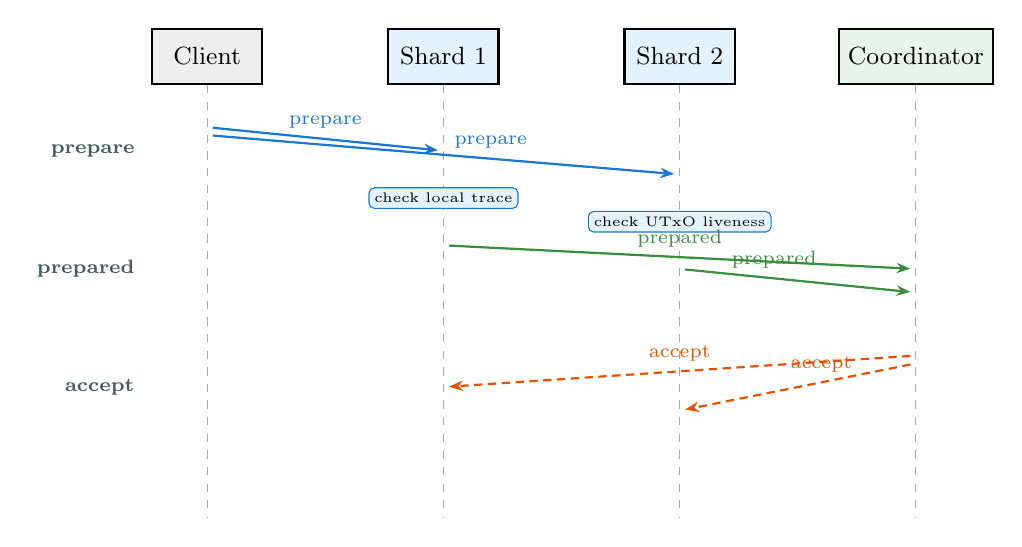
\begin{tikzpicture}[>=Stealth]
% Actor x-positions
\def\xClient{0}    \def\xSOne{3}
\def\xSTwo{6}      \def\xCoord{9}
% Phase y-positions
\def\yPrepare{-1.2}   \def\yPrepared{-2.7}   \def\yAccept{-4.2}

%% Actors
\node[actornode, fill=palGrayLt]  (client) at (\xClient, 0) {Client};
\node[actornode, fill=palBlueLt]  (s1)     at (\xSOne, 0)   {Shard 1};
\node[actornode, fill=palBlueLt]  (s2)     at (\xSTwo, 0)   {Shard 2};
\node[actornode, fill=palGreenLt] (coord)  at (\xCoord, 0)  {Coordinator};

%% Lifelines
\foreach \n in {client, s1, s2, coord} {
  \draw[dashed, palGray!50] (\n.south) -- ++(0, -5.5);
}

%% Phase Labels
\node[font=\scriptsize\bfseries, palGray, anchor=east] at (-0.8, \yPrepare)  {prepare};
\node[font=\scriptsize\bfseries, palGray, anchor=east] at (-0.8, \yPrepared) {prepared};
\node[font=\scriptsize\bfseries, palGray, anchor=east] at (-0.8, \yAccept)   {accept};

%% Messages — Phase 1: prepare
\draw[stdarrow, palBlue] (\xClient, -0.9) -- node[above, font=\scriptsize] {prepare} (\xSOne, \yPrepare);
\draw[stdarrow, palBlue] (\xClient, -1.0) -- node[above, font=\scriptsize, pos=0.6] {prepare} (\xSTwo, -1.5);

% Shard annotations
\node[rounded corners=2pt, fill=palBlueLt, draw=palBlue, font=\tiny, inner sep=2pt]
  at (\xSOne, -1.8) {check local trace};
\node[rounded corners=2pt, fill=palBlueLt, draw=palBlue, font=\tiny, inner sep=2pt]
  at (\xSTwo, -2.1) {check UTxO liveness};

%% Messages — Phase 2: prepared
\draw[stdarrow, palGreen] (\xSOne, -2.4) -- node[above, font=\scriptsize] {prepared} (\xCoord, \yPrepared);
\draw[stdarrow, palGreen] (\xSTwo, \yPrepared) -- node[above, font=\scriptsize, pos=0.4] {prepared} (\xCoord, -3.0);

%% Messages — Phase 3: accept
\draw[stdarrow, densely dashed, palOrange] (\xCoord, -3.8) -- node[above, font=\scriptsize] {accept} (\xSOne, \yAccept);
\draw[stdarrow, densely dashed, palOrange] (\xCoord, -3.9) -- node[above, font=\scriptsize, pos=0.4] {accept} (\xSTwo, -4.5);
\end{tikzpicture}
\caption{S-BAC prepare flow for ICE-UTxO. Dashed vertical lines are lifelines; three temporal phases flow top-to-bottom.}
\label{fig:sbac}
\end{figure}

%% ═══════════════════════════════════════════════════════════════════════════
\section{Operational Semantics and Ledger Safety}\label{sec:opsem}

This section defines how transactions change the ledger: a small-step operational semantics with eight constructors, two concurrency modes, and six invariants preserved by every step. All definitions and theorems are mechanized in \texttt{StarstreamPilot.lean}.

\subsection{Transaction Lifecycle}\label{sec:lifecycle}

A transaction proceeds through seven phases (Idle, Reserve, Executing, Committing, Committed, Rollback, Failed), driven by the step constructors below.

\begin{figure}[t]
\centering
\begin{adjustbox}{max width=\linewidth, center}
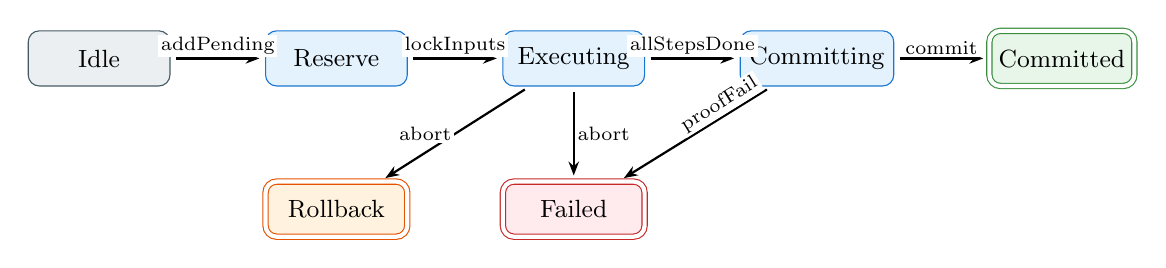
\begin{tikzpicture}[
  fsmst/.style={fsmstate, minimum width=1.8cm},
  >=Stealth,
  node distance=1.2cm
]
%% Happy Path Nodes
\node[fsmst, fill=palGrayLt, draw=palGray] (idle) {Idle};
\node[fsmst, fill=palBlueLt, draw=palBlue, right=of idle] (reserve) {Reserve};
\node[fsmst, fill=palBlueLt, draw=palBlue, right=of reserve] (exec) {Executing};
\node[fsmst, fill=palBlueLt, draw=palBlue, right=of exec] (commit) {Committing};
\node[fsmst, fill=palGreenLt, draw=palGreen, double, double distance=1.5pt, right=of commit] (done) {Committed};
%% Failure Nodes
\node[fsmst, fill=palOrangeLt, draw=palOrange, double, double distance=1.5pt, below=of reserve] (roll) {Rollback};
\node[fsmst, fill=palRedLt, draw=palRed, double, double distance=1.5pt, below=of exec] (fail) {Failed};
%% Transitions
\draw[stdarrow] (idle) -- node[above, font=\scriptsize, fill=white, inner sep=1pt] {addPending} (reserve);
\draw[stdarrow] (reserve) -- node[above, font=\scriptsize, fill=white, inner sep=1pt] {lockInputs} (exec);
\draw[stdarrow] (exec) -- node[above, font=\scriptsize, fill=white, inner sep=1pt] {allStepsDone} (commit);
\draw[stdarrow] (commit) -- node[above, font=\scriptsize, fill=white, inner sep=1pt] {commit} (done);
\draw[stdarrow] (exec) -- node[left, font=\scriptsize, fill=white, inner sep=1pt] {abort} (roll);
\draw[stdarrow] (exec) -- node[right, font=\scriptsize, fill=white, inner sep=1pt] {abort} (fail);
\draw[stdarrow] (commit) -- node[above, font=\scriptsize, fill=white, inner sep=1pt, sloped, pos=0.3] {proofFail} (fail);
\end{tikzpicture}
\end{adjustbox}
\caption{Transaction lifecycle state machine.}
\label{fig:lifecycle}
\end{figure}

\begin{definition}[Step]\label{def:step}
The small-step relation $\mathit{Step} : \mathit{Mode} \to \mathit{Ledger} \to \mathit{Ledger} \to \text{Prop}$ has eight constructors in three groups: \emph{lifecycle} (addPending, lockInputs, commit, abort) governs transaction admission, resource reservation, finalization, and failure; \emph{effect} (installH, uninstallH, raiseE, handleE) implements the algebraic-effects paradigm at the ledger level; and the lifecycle constructors carry the mode-sensitive preconditions that enforce concurrency control.
\end{definition}

\begin{table}[t]
\caption{Step constructors of the ICE-UTxO operational semantics.}
\label{tab:step-constructors}
\centering\small
\begin{tabular}{lllll}
\toprule
\textbf{Constructor} & \textbf{Mode} & \textbf{Precondition} & \textbf{Effect} & \textbf{Intuition} \\
\midrule
\texttt{addPending} & any & $\mathit{tx} \notin L.\mathit{pending}$, \texttt{noDupProofs} & Add to pending & Submit for consideration \\
\texttt{lockInputs} & locking & $\mathit{tx} \in \mathit{pending}$, inputs disjoint, live & Lock inputs & Reserve inputs (pessimistic) \\
\texttt{commit} & any & \texttt{commitEnabledStrong}, acyclicity & Apply commit & Finalize---strongest gate \\
\texttt{abort} & any & $\mathit{tx} \in \mathit{pending}$ & Release locks & Graceful failure / timeout \\
\texttt{installH} & any & (none) & Push handler & Register effect handler \\
\texttt{uninstallH} & any & (none) & Pop handler & Deregister effect handler \\
\texttt{raiseE} & any & (none) & Push effect & Request cross-boundary service \\
\texttt{handleE} & any & effect + handler present & Route effect & Dispatch to registered handler \\
\bottomrule
\end{tabular}
\end{table}

\paragraph{Entry gate: \texttt{addPending}.} Preconditions ($\mathit{tx} \notin L.\mathit{pending}$, \texttt{noDupProofs}) are deliberately minimal; all semantic validation is deferred to later phases. This makes \texttt{addPending} the primary DoS surface; mitigation via fees or rate limiting is essential in deployment but outside the model's scope.

\paragraph{Pessimistic reserve: \texttt{lockInputs}.} Inputs must be disjoint from already-locked UTxOs and live, mirroring strict two-phase locking (S2PL).

\paragraph{Terminal gate: \texttt{commit}.} The strongest preconditions: $\mathit{allProofsVerified}$, $\mathit{validTx}$, committing phase, pending and not in history. Acyclicity predicates are tautologically satisfied (\cref{sec:precedence}).

\paragraph{Graceful failure: \texttt{abort}.} Any pending transaction may abort at any time (nondeterministic), modeling timeouts and cancellation. Safety is ``only valid transactions \emph{can} commit,'' not ``valid transactions must commit.''

\paragraph{Effect quartet: \texttt{installH}, \texttt{uninstallH}, \texttt{raiseE}, \texttt{handleE}.} These four constructors implement algebraic effects at the ledger level. Only \texttt{handleE} has a precondition (both a pending effect and a handler must be present). If a handler is uninstalled while effects are pending, the effects remain unrouted and the transaction must abort or install a replacement. The commit guard does not explicitly check for unresolved effects; effect resolution is enforced through the IVC proof (\cref{rem:ivc-predicate}), conditional on SA1.

\begin{definition}[State Updates]\label{def:state-updates}
\begin{align*}
\mathit{applyCommit}(L, \mathit{tx}) &= L\Big[\mathit{utxos} := (L.\mathit{utxos} \setminus \mathit{tx.inputs}) \cup \mathit{tx.outputs},\\
&\quad\; \mathit{consumed} := L.\mathit{consumed} \cup \mathit{tx.inputs},\\
&\quad\; \mathit{locked} := L.\mathit{locked} \setminus \mathit{tx.inputs},\\
&\quad\; \mathit{pending} := L.\mathit{pending} \setminus \{\mathit{tx}\},\\
&\quad\; \mathit{history} := L.\mathit{history} \mathbin{+\!\!+} [\mathit{tx}]\Big]
\end{align*}
\begin{align*}
\mathit{applyAbort}(L, \mathit{tx}) &= L\Big[\mathit{locked} := L.\mathit{locked} \setminus \mathit{tx.inputs},\;
\mathit{pending} := L.\mathit{pending} \setminus \{\mathit{tx}\}\Big]
\end{align*}
\end{definition}

\begin{definition}[Multi-Step]\label{def:multi-step}
$\mathit{Steps} : \mathit{Mode} \to \mathit{Ledger} \to \mathit{Ledger} \to \text{Prop}$ is the reflexive-transitive closure of $\mathit{Step}$.
\end{definition}

\subsection{Commit Rule and Proof-Gating}\label{sec:commit-rule}

The commit rule enforces that only proof-verified, structurally valid transactions can extend the ledger history.

\begin{definition}[All Proofs Verified]\label{def:all-proofs-verified}
$\mathit{allProofsVerified}(\mathit{tx}) \iff \mathit{tx.proofCommitments} \neq [] \wedge \forall p \in \mathit{tx.proofCommitments}.\; p.\mathit{phase} = \text{Verified}$
\end{definition}

\paragraph{Trust boundary.} The predicate $\mathit{allProofsVerified}$ checks phase flags set by an external ZK verifier. Cryptographic soundness---that a \texttt{Verified} flag genuinely corresponds to a valid ZK proof---is outside the scope of this formalization. The model proves: \emph{if} the verifier sets flags correctly, \emph{then} the ledger maintains its invariants.

\paragraph{IVC proof failure.} Any single proof failure prevents commit; the transaction must abort and retry. No partial-proof recovery exists.

\paragraph{Security assumptions.} The commit rule relies on SA1--SA3 (\cref{sec:state-components}). The \texttt{Step} relation does not constrain constructor ordering; safety proofs hold for the full state space including ill-phased interleavings.

\begin{definition}[Valid Transaction]\label{def:valid-tx}
$\mathit{validTx}(L, \mathit{tx})$ requires:
\begin{itemize}
  \item $\mathit{tx.inputs} \neq \emptyset$ and $\mathit{tx.outputs} \neq \emptyset$
  \item $\mathit{tx.inputs} \cap \mathit{tx.outputs} = \emptyset$ (inputs disjoint from outputs)
  \item $\mathit{tx.inputs} \subseteq L.\mathit{utxos}$ (inputs are live)
  \item $\mathit{tx.outputs} \cap (L.\mathit{utxos} \cup L.\mathit{consumed}) = \emptyset$ (outputs are fresh)
\end{itemize}
\end{definition}

\begin{remark}[Non-empty inputs]\label{rem:nonempty-inputs}
The requirement $\mathit{tx.inputs} \neq \emptyset$ excludes coinbase and minting transactions. The serializability proof (\cref{sec:serializability}) relies on every committed transaction inducing at least one conflict edge.
\end{remark}

\begin{definition}[Commit Enabled---Strong]\label{def:commit-enabled}
$\mathit{commitEnabledStrong}(m, L, \mathit{tx})$ holds if:
\[
\mathit{allProofsVerified}(\mathit{tx}) \wedge \mathit{validTx}(L, \mathit{tx}) \wedge \mathit{tx.phase} = \text{Committing} \wedge \mathit{tx} \notin L.\mathit{history}
\]
and additionally:
\begin{itemize}
  \item \textbf{Locking mode}: $\mathit{tx.inputs} \subseteq L.\mathit{locked}$ and $\mathit{tx.readSet} \subseteq L.\mathit{utxos}$.
  \item \textbf{Optimistic mode}: $\mathit{tx.readSet} \subseteq L.\mathit{utxos}$ and $\mathit{tx.outputs}$ are fresh.
\end{itemize}
\end{definition}

\begin{theorem}[Proof-Gated Commit]\label{thm:proof-gated}
Any step that extends the history requires proof verification:
\[
\mathit{Step}(m, L, L') \wedge L'.\mathit{history} = L.\mathit{history} \mathbin{+\!\!+} [\mathit{tx}] \implies \mathit{proofOk}(\mathit{tx})
\]
\emph{(Mechanized: \texttt{commit\_requires\_proof}, StarstreamPilot.lean.)}
\end{theorem}

\begin{proof}[Proof sketch]
Exhaustive case analysis on the eight \texttt{Step} constructors. Seven non-commit constructors leave the history unchanged, yielding a contradiction with the hypothesis via the lemma $\mathit{xs} \neq \mathit{xs} \mathbin{+\!\!+} [x]$. The commit constructor directly provides $\mathit{allProofsVerified}(\mathit{tx})$ from $\mathit{commitEnabledStrong}$.
\end{proof}

\subsection{Concurrency Modes}\label{sec:concurrency-modes}

ICE-UTxO supports two concurrency modes, selected per-transaction:

\paragraph{Locking mode} ($m = \text{locking}$). Inputs are reserved before execution via the \texttt{lockInputs} step, which requires $\mathit{tx.inputs} \cap L.\mathit{locked} = \emptyset$ (no double-locking) and $\mathit{tx.inputs} \subseteq L.\mathit{utxos}$ (inputs live). At commit time, the commit guard checks $\mathit{tx.inputs} \subseteq L.\mathit{locked}$.

\paragraph{Optimistic mode} ($m = \text{optimistic}$). No locks are acquired. At commit time, the guard checks that the read snapshot is still valid ($\mathit{tx.readSet} \subseteq L.\mathit{utxos}$) and outputs are still fresh. If the snapshot has been invalidated by a concurrent commit, the transaction fails.

Both modes are proof-gated: $\mathit{allProofsVerified}$ is required regardless of the concurrency mode.

\paragraph{Adversarial contention.} Under adversarial contention in optimistic mode, abort rates can approach 100\%. Liveness under contention requires fairness assumptions (\cref{sec:liveness}).

\paragraph{Comparative analysis.} Ethereum uses sequential execution under a global lock; Sui~\cite{Blackshear2023} achieves parallelism via Move's linear types; Cosmos~\cite{Kwon2019} isolates state per chain. ICE-UTxO offers per-transaction mode selection within a single ledger, with proof-gated commit and algebraic effects for multi-step coordination.

\subsection{Ledger Invariants}\label{sec:ledger-invariants}

\begin{definition}[Ledger Invariant]\label{def:ledger-invariant}
$\mathit{ledgerInvariant}(L)$ is the conjunction of four safety components: (1)~no double-spend; (2)~locked subset active; (3)~history nodup; (4)~committed implies verified. The Lean mechanization includes two additional structural components---extended precedence acyclic and full precedence acyclic---that hold tautologically for any list-indexed history (\cref{sec:precedence}) and serve as witnesses for the serializability precondition.
\end{definition}

\begin{theorem}[Invariant Preservation]\label{thm:invariant-preservation}
Every step preserves the ledger invariant:
\[
\mathit{Step}(m, L, L') \wedge \mathit{ledgerInvariant}(L) \implies \mathit{ledgerInvariant}(L')
\]
\emph{(Mechanized: \texttt{step\_preserves\_invariant}, StarstreamPilot.lean.)}
\end{theorem}

\begin{proof}[Proof sketch]
Floyd-Hoare style case analysis on the eight \texttt{Step} constructors. \texttt{addPending}, \texttt{installH}, \texttt{uninstallH}, \texttt{raiseE}, \texttt{handleE} do not modify $\mathit{utxos}$, $\mathit{consumed}$, or $\mathit{history}$, so all six invariant components are trivially preserved. \texttt{lockInputs}: $\mathit{locked}$ grows by $\mathit{tx.inputs}$, which are live ($\subseteq L.\mathit{utxos}$), preserving \texttt{lockedSubsetActive}. \texttt{abort}: $\mathit{locked}$ shrinks. \texttt{commit}: no-double-spend follows from \texttt{commit\_preserves\_no\_double\_spend}; history nodup from the freshness guard $\mathit{tx} \notin L.\mathit{history}$; acyclicity from the commit step's preconditions.
\end{proof}

\paragraph{Lock lifetime and deadlock prevention.} The formalization imposes no lock expiration: locks persist until the holding transaction commits or aborts. This is deliberate---the model captures the worst case (unbounded lock duration) so that safety proofs do not depend on timing assumptions. In practice, a deployment must enforce lock timeouts to prevent indefinite lock holding; any timeout policy can be implemented as an external abort trigger, and the model's safety properties are preserved under \emph{any} abort policy, since the \texttt{abort} constructor is unconditionally available (\cref{thm:progress}).

Deadlock among locking-mode transactions cannot arise under a simple discipline: if all transactions acquire locks in a fixed total order over UTxO identifiers, the resulting lock-acquisition graph is acyclic. The \texttt{lockInputs} precondition ($\mathit{tx.inputs} \cap L.\mathit{locked} = \emptyset$) already prevents a transaction from acquiring a lock held by another, which forces the failing transaction to abort and retry---effectively converting potential deadlocks into aborts. The unconditional abort constructor is a safety valve: any transaction that cannot acquire its locks will eventually abort under $\mathit{WF}(\text{abort})$ (\cref{sec:liveness}), releasing its held locks for others.

\begin{theorem}[No Double-Spend Preservation]\label{thm:no-double-spend}
$\mathit{noDoubleSpend}(L) \wedge \mathit{outputsFresh}(L, \mathit{tx}) \wedge \mathit{inputsLive}(L, \mathit{tx}) \implies \mathit{noDoubleSpend}(\mathit{applyCommit}(L, \mathit{tx}))$.
\emph{(Mechanized: \texttt{commit\_preserves\_no\_double\_spend}.)}
\end{theorem}

\begin{theorem}[Consumed Monotonicity]\label{thm:consumed-monotone}
$\mathit{Step}(m, L, L') \implies L.\mathit{consumed} \subseteq L'.\mathit{consumed}$. This extends to multi-step: $\mathit{Steps}(m, L_0, L_n) \implies L_0.\mathit{consumed} \subseteq L_n.\mathit{consumed}$.
\emph{(Mechanized: \texttt{consumed\_monotone\_step}, \texttt{consumed\_monotone\_steps}.)}
\end{theorem}

\begin{theorem}[Progress]\label{thm:progress}
Any pending transaction can take a step (at minimum via abort):
$\mathit{tx} \in L.\mathit{pending} \implies \exists L'.\; \mathit{Step}(m, L, L')$.
\emph{(Mechanized: \texttt{pending\_can\_step}.)}
\end{theorem}

\subsection{Reduction to eUTxO}\label{sec:reduction}

\begin{proposition}[Conservative Extension]\label{prop:conservative-extension}
There exists a structure-preserving embedding $\iota : \mathit{Ledger}_{\text{eUTxO}} \to \mathit{Ledger}_{\text{ICE}}$ such that for every eUTxO step $L \xrightarrow{s} L'$, the lifted step $\iota(L) \xrightarrow{s'} \iota(L')$ is a valid ICE-UTxO step, and conversely, every ICE-UTxO safety property (no double-spend, input liveness, output freshness) restricted to the image of $\iota$ coincides with the corresponding eUTxO property.
\end{proposition}

\begin{proof}[Proof sketch]
The embedding $\iota$ maps an eUTxO state to ICE-UTxO with empty handler stacks, empty effect queues, and trivial proof commitments. The effect and coroutine machinery is inert; the transaction commits atomically in a single step. Safety properties transfer directly (\cref{thm:invariant-preservation,thm:no-double-spend,thm:consumed-monotone}). Fully mechanized in \texttt{ConservativeExtension.lean}: embedding, step-lifting, safety coincidence, and commit guard degeneration are all proved.
\end{proof}

\begin{corollary}\label{cor:conservative-degenerate}
For embedded eUTxO transactions, $\mathit{commitEnabledStrong}$ reduces to: inputs live, outputs fresh, inputs disjoint from outputs, and proof verified---exactly the standard eUTxO validation conditions.
\end{corollary}

\subsection{Conditional Liveness}\label{sec:liveness}

This section establishes conditional liveness under explicit fairness assumptions. Supporting lemmas are mechanized in Lean; the liveness theorems are paper-level arguments validated by TLC model checking.

\subsubsection{Fairness Assumptions}\label{sec:fairness}

We adopt Lamport's temporal logic of actions (TLA)~\cite{Lamport1994} to state fairness conditions. For an action~$A$:
\begin{itemize}
  \item \textbf{Weak fairness} $\mathit{WF}(A)$: if $A$ is continuously enabled, it eventually fires. Formally, $\Box(\Box\,\mathit{ENABLED}(A) \Rightarrow \Diamond A)$.
  \item \textbf{Strong fairness} $\mathit{SF}(A)$: if $A$ is infinitely often enabled, it eventually fires. Formally, $\Box(\Box\Diamond\,\mathit{ENABLED}(A) \Rightarrow \Diamond A)$.
\end{itemize}
We assume: (1)~$\mathit{WF}(\text{commit})$: if commit is continuously enabled, the scheduler eventually executes it. (2)~$\mathit{WF}(\text{abort})$: if a transaction remains pending, the scheduler eventually aborts it. (3)~$\mathit{WF}(\text{handleE})$: if effect handling is continuously enabled, the scheduler eventually dispatches it.

\paragraph{Deployment interpretation.} $\mathit{WF}(\text{commit})$ is enforced by block-production schedules; $\mathit{WF}(\text{abort})$ by timeout mechanisms that garbage-collect stalled transactions; $\mathit{WF}(\text{handleE})$ by live effect-routing. When any assumption is violated, the system degrades predictably: safety invariants (\cref{thm:invariant-preservation}) continue to hold, but liveness degrades (throughput stalls, lock exhaustion, or coroutine deadlock, respectively).

\subsubsection{Ledger-Level Progress (L1, L2)}\label{sec:ledger-progress}

\begin{theorem}[Eventual Commit Under Stability (L1)]\label{thm:L1}
Under $\mathit{WF}(\text{commit})$, if a transaction $\mathit{tx}$ remains pending and $\mathit{commitEnabledStrong}$ holds continuously (including both acyclicity conditions), then $\mathit{tx}$ eventually commits.
\end{theorem}

\begin{proof}[Proof sketch]
By \texttt{commit\_step\_specific} (Lean), the commit step for $\mathit{tx}$ exists in every state where the preconditions hold. Continuous enabledness plus $\mathit{WF}(\text{commit})$ forces the step to fire. By \texttt{commit\_adds\_to\_history}, $\mathit{tx}$ enters the history. By \texttt{commit\_removes\_from\_pending}, $\mathit{tx}$ leaves the pending set.
\end{proof}

\begin{theorem}[Eventual Terminalization (L2)]\label{thm:L2}
Under $\mathit{WF}(\text{abort})$, every pending transaction eventually either commits or leaves the pending set.
\end{theorem}

\begin{proof}[Proof sketch]
By \texttt{abort\_enabled\_of\_pending}, abort is always enabled for any pending transaction. Under $\mathit{WF}(\text{abort})$, the abort step eventually fires unless another step removes $\mathit{tx}$ from pending first. By \texttt{abort\_removes\_from\_pending}, abort removes $\mathit{tx}$ from the pending set.
\end{proof}

\subsubsection{Effect-Handling Progress (L3)}\label{sec:effect-progress}

\begin{theorem}[Effect Handling Progress (L3)]\label{thm:L3}
Under $\mathit{WF}(\text{handleE})$ for interface $i$, if a handler remains installed on $i$ and effects are pending on $i$, then the effect queue for $i$ eventually empties.
\end{theorem}

\begin{proof}[Proof sketch]
By \texttt{handleEffect\_succeeds}, \texttt{handleE} is enabled when both an effect and a handler are present. By \texttt{handleEffect\_decreases\_effects}, each \texttt{handleE} step strictly decreases the effect queue length. The queue length is a natural number, so by well-founded induction the queue empties after at most $n$ steps.
\end{proof}

\subsubsection{Coordination and Cross-Shard Progress (L4, L5)}\label{sec:cross-shard-progress}

\begin{proposition}[Coordination Completion (L4)]\label{prop:L4}
If a PTB program is conflict-free and all roles participate fairly, the induced event-structure trace can be extended to a complete configuration.
\end{proposition}

\begin{proof}[Argument]
By \texttt{toScript\_wellFormed}, the induced event structure has acyclic order. In any well-formed event structure, every non-maximal configuration has an enabled event. Under fair role participation, enabled events are eventually executed. The trace extends until maximal. This follows the global progress argument of Coppo et al.~\cite{Coppo2016} instantiated in the event-structure setting of Castellani et al.~\cite{Castellani2023}.
\end{proof}

\begin{remark}[Cross-Shard Termination (L5)]\label{rem:L5}
Under partial synchrony (DLS model) with $f_s < n_s/3$ per shard, S-BAC eventually decides. This is a direct consequence of BFT consensus liveness per shard~\cite{Dwork1988} combined with the non-blocking atomic commit structure~\cite{AlBassam2018}. Cross-shard deadlock cannot arise; the structural argument is given in \cref{sec:coordination-witness}.
\end{remark}

\subsubsection{Model Checking Validation}\label{sec:model-checking}

TLC model checking found no counterexamples in state spaces up to MAX\_UTXOS=3, MAX\_PENDING\_TXS=2 (${\sim}10^6$ states, ${\sim}45$~min on 16~cores), exercising all eight step constructors, both concurrency modes, and the full effect-handling lifecycle. This provides counterexample-search confidence, not proof-level confidence. The TLA+ specification defines \texttt{FairSpec} (weak fairness on commit, abort, rollback) and \texttt{StrongFairSpec} (additional strong fairness on \texttt{HandleTxEffect}); TLC confirms all four liveness properties hold. The full TLA+ treatment appears in \cref{sec:tla-architecture,sec:cross-artifact}.

\subsection{Safety vs.\ Liveness Summary}\label{sec:safety-liveness-summary}

\begin{table}[t]
\caption{Safety and liveness properties of ICE-UTxO. ``Lean'' = mechanized proof; ``TLC'' = model-checked on bounded instances; ``Paper'' = paper-level argument with mechanized support lemmas.}
\label{tab:safety-liveness}
\centering\small
\begin{tabular}{p{4.2cm}ccl}
\toprule
\textbf{Property} & \textbf{Kind} & \textbf{Status} & \textbf{Reference} \\
\midrule
No double spend & Safety & Lean & Thm.~\ref{thm:no-double-spend} \\
Invariant preservation & Safety & Lean & Thm.~\ref{thm:invariant-preservation} \\
Proof-gated commit & Safety & Lean & Thm.~\ref{thm:proof-gated} \\
Conservative extension & Safety & Lean & Prop.~\ref{prop:conservative-extension} \\
Conflict serializability & Safety & Lean & Thm.~\ref{thm:strong-serial} \\
Concurrent-to-serial refinement & Safety & Lean & Thm.~\ref{thm:concurrent-refines-serial} \\
Global $\Leftrightarrow$ local witness & Safety & Lean & Thm.~\ref{thm:global-implies-local}, \ref{thm:consistent-implies-global} \\
\addlinespace
Eventual commit (L1) & Liveness & Paper+TLC & Thm.~\ref{thm:L1} \\
Eventual termination (L2) & Liveness & Paper+TLC & Thm.~\ref{thm:L2} \\
Eventual effect handling (L3) & Liveness & Paper+TLC & Thm.~\ref{thm:L3} \\
Coordination completion (L4) & Liveness & Paper & Prop.~\ref{prop:L4} \\
Cross-shard termination (L5) & Liveness & Paper & Rem.~\ref{rem:L5} \\
\bottomrule
\end{tabular}
\end{table}

\Cref{tab:safety-liveness} summarizes the properties. Safety is proved universally in Lean; liveness is conditional on fairness and validated by TLC on bounded instances.

%% ═══════════════════════════════════════════════════════════════════════════
\section{Conflict Serializability}\label{sec:serializability}

In a sharded ledger, different shards may apply transactions in different orders. Conflict serializability guarantees that all conflict-respecting orderings produce the same final state, preventing divergence on asset ownership.

Classical conflict serializability~\cite{Papadimitriou1986,Bernstein1987} shows that acyclic conflict graphs admit \emph{some} equivalent serial order. The result here is stronger: \emph{all} conflict-respecting permutations produce \emph{identical} core state. This universal quantification is necessary for sharded execution, where every shard must arrive at the same state regardless of which valid ordering it uses. The proof uses the bubble-sort / adjacent-swap method from Mazurkiewicz trace theory~\cite{Mazurkiewicz1987}, mechanized end-to-end in Lean. The deterministic-transaction assumption (state transitions depend only on declared inputs, outputs, and readSet) makes the conflict relation complete: any pair not captured by $\mathit{fullConflicts}$ (\cref{def:full-conflicts}) can be reordered without affecting core state.

\subsection{Precedence Graph and Conflict Relations}\label{sec:precedence}

\begin{definition}[Conflicts]\label{def:conflicts}
Two transactions conflict if they have overlapping read/write sets:
\[
\mathit{conflicts}(t_1, t_2) \iff (t_1.\mathit{writeSet} \cap t_2.\mathit{readSet}) \neq \emptyset \;\lor\; (t_1.\mathit{readSet} \cap t_2.\mathit{writeSet}) \neq \emptyset \;\lor\; (t_1.\mathit{writeSet} \cap t_2.\mathit{writeSet}) \neq \emptyset
\]
\end{definition}

\begin{definition}[Full Conflicts]\label{def:full-conflicts}
\begin{align*}
\mathit{fullConflicts}(t_1, t_2) \iff{} & \mathit{conflicts}(t_1, t_2) \lor \mathit{conflicts}(t_2, t_1)\\
\lor{} & (t_1.\mathit{outputs} \cap t_2.\mathit{inputs}) \neq \emptyset \\
\lor{} & (t_2.\mathit{outputs} \cap t_1.\mathit{inputs}) \neq \emptyset \\
\lor{} & (t_1.\mathit{outputs} \cap t_2.\mathit{outputs}) \neq \emptyset
\end{align*}
\end{definition}

The relation is deliberately broad: any pair not flagged by $\mathit{fullConflicts}$ can be applied in either order with identical core-state results (\cref{thm:core-commute}).

\begin{theorem}[Symmetry]\label{thm:full-conflicts-symm}
$\mathit{fullConflicts}(t_1, t_2) \implies \mathit{fullConflicts}(t_2, t_1)$, by commutativity of set intersection and the symmetry of the five disjuncts.
\emph{(Mechanized: \texttt{fullConflicts\_symm}.)}
\end{theorem}

\begin{definition}[Precedence]\label{def:precedence}
For a history $\mathit{hist}$, define $\mathit{before}(\mathit{hist}, t_1, t_2) \iff \mathit{idxOf}(t_1) < \mathit{idxOf}(t_2)$ and:
\[
\mathit{fullPrecEdge}(\mathit{hist}, t_1, t_2) \iff \mathit{before}(\mathit{hist}, t_1, t_2) \wedge \mathit{fullConflicts}(t_1, t_2)
\]
\end{definition}

\begin{definition}[Acyclicity]\label{def:acyclicity}
$\mathit{fullPrecGraphAcyclic}(\mathit{hist}) \iff \forall t.\; \neg\, \mathit{TransGen}(\mathit{fullPrecEdge}(\mathit{hist}))(t, t)$.
\end{definition}

Since $\mathit{before}$ is defined by list index, any list induces a DAG: acyclicity holds unconditionally for every history (\texttt{fullPrecGraphAcyclic\_of\_history}). The acyclicity components appear in the ledger invariant as structural witnesses recording that the serializability precondition (\cref{thm:strong-serial}) is satisfied by construction; the substantive safety content resides in components 1--4.

\subsection{Core State Abstraction and Commutativity}\label{sec:core-state}

Projecting away the history yields a \emph{core state} (UTxO set and consumed set only) where non-conflicting commits can be shown to commute. The full ledger's history list is inherently order-dependent; on the core projection, commutativity becomes tractable.

\begin{definition}[Core State]\label{def:core-state}
$\mathit{CoreState} = (\mathit{utxos} : \Pfin(\mathit{UTXOId}),\; \mathit{consumed} : \Pfin(\mathit{UTXOId}))$. The projection $\mathit{coreOf}(L) = (L.\mathit{utxos}, L.\mathit{consumed})$ extracts core state from a ledger.
\end{definition}

\begin{definition}[Core Commit]\label{def:core-commit}
$\mathit{applyCoreCommit}(s, \mathit{tx}) = ((s.\mathit{utxos} \setminus \mathit{tx.inputs}) \cup \mathit{tx.outputs},\; s.\mathit{consumed} \cup \mathit{tx.inputs})$.
\end{definition}

\begin{theorem}[Core Commutativity]\label{thm:core-commute}
Non-conflicting transactions commute at the core state level:
\[
\neg\,\mathit{fullConflicts}(t_1, t_2) \implies \mathit{applyCoreCommit}(\mathit{applyCoreCommit}(s, t_1), t_2) = \mathit{applyCoreCommit}(\mathit{applyCoreCommit}(s, t_2), t_1)
\]
\emph{(Mechanized: \texttt{core\_commute}, StarstreamPilot.lean.)}
\end{theorem}

\begin{proof}[Proof sketch]
From the five negated disjuncts of $\neg\,\mathit{fullConflicts}$, we extract $t_1.\mathit{outputs} \cap t_2.\mathit{inputs} = \emptyset$ and $t_2.\mathit{outputs} \cap t_1.\mathit{inputs} = \emptyset$. The proof proceeds by extensional reasoning on \texttt{Finset} membership for both components. For \texttt{utxos}: $((A \setminus B_1) \cup C_1) \setminus B_2) \cup C_2 = ((A \setminus B_2) \cup C_2) \setminus B_1) \cup C_1$ when $C_1 \cap B_2 = \emptyset$ and $C_2 \cap B_1 = \emptyset$. For \texttt{consumed}: union is commutative and associative.
\end{proof}

Commutativity is tractable on $\mathit{CoreState}$ because commits reduce to set operations on disjoint elements.

\begin{theorem}[Adjacent Swap]\label{thm:adjacent-swap}
Swapping adjacent non-conflicting transactions preserves core history:
\[
\neg\,\mathit{fullConflicts}(t_1, t_2) \implies \mathit{applyCoreHistory}(s, \mathit{pre} \mathbin{+\!\!+} [t_1, t_2] \mathbin{+\!\!+} \mathit{suf}) = \mathit{applyCoreHistory}(s, \mathit{pre} \mathbin{+\!\!+} [t_2, t_1] \mathbin{+\!\!+} \mathit{suf})
\]
\emph{(Mechanized: \texttt{core\_swap\_nonconflicting}.)}
\end{theorem}

\subsection{Strong Serializability via Bubble-Sort}\label{sec:bubble-sort}

We now build the machinery to prove that \emph{all} conflict-respecting permutations produce the same core state.

\begin{definition}[Conflict Equivalence]\label{def:conflict-equiv}
The inductive relation $\mathit{ConflictEquiv}$ on transaction lists is generated by reflexivity, adjacent swap of non-conflicting transactions, and transitivity.
\end{definition}

\begin{theorem}[Conflict Equivalence Preserves Core State]\label{thm:conflict-equiv-core}
$\mathit{ConflictEquiv}(\ell_1, \ell_2) \implies \mathit{applyCoreHistory}(s, \ell_1) = \mathit{applyCoreHistory}(s, \ell_2)$.
\emph{(Mechanized: \texttt{conflict\_equiv\_same\_core}.)}
\end{theorem}

\begin{lemma}[Bubble Past Suffix]\label{lem:bubble-past}
If $t$ does not fully conflict with any element of $\mathit{suf}$, then $\mathit{ConflictEquiv}(\mathit{pre} \mathbin{+\!\!+} [t] \mathbin{+\!\!+} \mathit{suf},\; \mathit{pre} \mathbin{+\!\!+} \mathit{suf} \mathbin{+\!\!+} [t])$.
\emph{(Mechanized: \texttt{bubble\_past\_suffix}.)}
\end{lemma}

\begin{figure}[t]
\centering
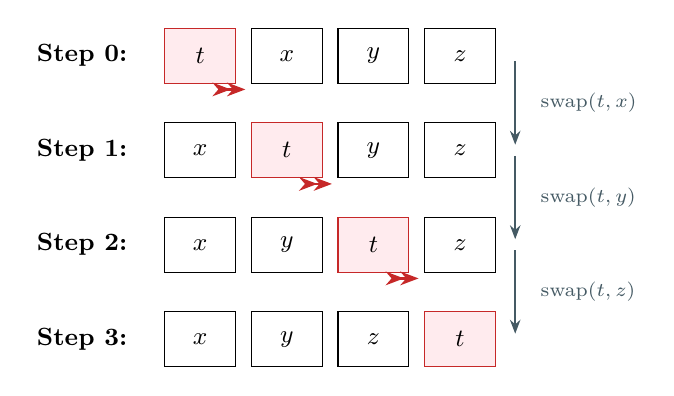
\begin{tikzpicture}[>=Stealth]
\def\xLabel{-1.5}   % x-position for step labels
\def\xBox{1.1}      % horizontal spacing between boxes
\def\yStart{2}       % y-position of first row
\def\yStep{1.2}      % vertical spacing between rows
\def\xTrans{4.0}     % x-position for transition arrows
\def\xTransLbl{4.2}  % x-position for transition labels

%% Nodes — each row: step index / t-position / labels left-to-right
\foreach \step/\tpos/\lblA/\lblB/\lblC/\lblD in {
  0/0/t/x/y/z,
  1/1/x/t/y/z,
  2/2/x/y/t/z,
  3/3/x/y/z/t%
} {
  \pgfmathsetmacro{\yrow}{\yStart - \step*\yStep}
  \node[font=\small\bfseries] at (\xLabel, \yrow) {Step \step:};
  \foreach \col/\lbl in {0/\lblA, 1/\lblB, 2/\lblC, 3/\lblD} {
    \pgfmathsetmacro{\xpos}{\col*\xBox}
    \ifnum\col=\tpos\relax
      \node[sortbox, fill=palRedLt, draw=palRed] (\lbl\step) at (\xpos, \yrow) {$\lbl$};
    \else
      \node[sortbox] (\lbl\step) at (\xpos, \yrow) {$\lbl$};
    \fi
  }
}

%% Swap Arrows (steps 0–2: t swaps with its right neighbour)
\foreach \step/\swapWith in {0/x, 1/y, 2/z} {
  \draw[stdarrow, palRed, <->] ([yshift=-2pt]t\step.south east) -- ([yshift=-2pt]\swapWith\step.south west);
}

%% Step Transition Arrows and Labels
\foreach \step/\partner in {0/x, 1/y, 2/z} {
  \pgfmathsetmacro{\yhi}{\yStart - \step*\yStep}
  \pgfmathsetmacro{\ylo}{\yStart - (\step+1)*\yStep}
  \pgfmathsetmacro{\ymid}{(\yhi+\ylo)/2}
  \draw[stdarrow, palGray] (\xTrans, \yhi) -- (\xTrans, \ylo);
  \node[font=\scriptsize, palGray, anchor=west] at (\xTransLbl, \ymid) {swap$(t,\partner)$};
}
\end{tikzpicture}
\caption{Bubble-sort swap illustration. Transaction $t$ (highlighted) does not conflict with $x$, $y$, or $z$, so iterated adjacent transpositions move $t$ to the end.}
\label{fig:bubble-sort}
\end{figure}

\begin{definition}[Respects Conflict Order]\label{def:respects-conflict}
$\mathit{respectsConflictOrder}(\mathit{order}, \mathit{hist}) \iff \forall t_1, t_2.\; \mathit{fullConflicts}(t_1, t_2) \wedge \mathit{before}(\mathit{hist}, t_1, t_2) \implies \mathit{before}(\mathit{order}, t_1, t_2)$
\end{definition}

\begin{definition}[Strong Core Serializability]\label{def:strong-serial}
$\mathit{strongCoreSerializable}(s_0, \mathit{hist}) \iff \forall \mathit{order}.\; \mathit{Perm}(\mathit{order}, \mathit{hist}) \wedge \mathit{respectsConflictOrder}(\mathit{order}, \mathit{hist}) \implies \mathit{applyCoreHistory}(s_0, \mathit{order}) = \mathit{applyCoreHistory}(s_0, \mathit{hist})$
\end{definition}

Conflict-respecting permutations are executable: if transaction~$B$ consumes an output of~$A$, then $\mathit{fullConflicts}(A, B)$ holds, and $\mathit{respectsConflictOrder}$ forces $A$ before $B$ in every considered permutation. Every causal dependency is captured by a conflict edge.

\begin{theorem}[Acyclic Implies Strong Serializability]\label{thm:strong-serial}
\[
\mathit{hist.Nodup} \wedge \mathit{fullPrecGraphAcyclic}(\mathit{hist}) \implies \mathit{strongCoreSerializable}(s_0, \mathit{hist})
\]
\emph{(Mechanized: \texttt{acyclic\_strong\_serializable}, StarstreamPilot.lean.)}
\end{theorem}

\begin{proof}[Proof]
By strong induction on $|\mathit{hist}|$ using \texttt{List.reverseRecOn} (which decomposes the list by peeling the last element, aligning the Lean proof structure with the paper's ``bubble to end'' argument).

\emph{Base case} ($\mathit{hist} = []$): any permutation of $[]$ is $[]$; trivial.

\emph{Inductive case} ($\mathit{hist} = \mathit{init} \mathbin{+\!\!+} [t]$): given a conflict-respecting permutation $\mathit{order}$ of $\mathit{init} \mathbin{+\!\!+} [t]$:

\begin{enumerate}
  \item \textbf{Locate $t$}: since $t \in \mathit{order}$, write $\mathit{order} = \mathit{pre} \mathbin{+\!\!+} [t] \mathbin{+\!\!+} \mathit{suf}$.

  \item \textbf{Suffix is non-conflicting}: for each $x \in \mathit{suf}$, we have $\mathit{before}(\mathit{order}, t, x)$. If $\mathit{fullConflicts}(t, x)$ held, then by symmetry $\mathit{fullConflicts}(x, t)$, and since $x \in \mathit{init}$ we would have $\mathit{before}(\mathit{hist}, x, t)$, so $\mathit{respectsConflictOrder}$ would force $\mathit{before}(\mathit{order}, x, t)$---contradicting $\mathit{before}(\mathit{order}, t, x)$.

  \item \textbf{Bubble $t$ to end}: by \cref{lem:bubble-past}, $\mathit{ConflictEquiv}(\mathit{order}, \mathit{pre} \mathbin{+\!\!+} \mathit{suf} \mathbin{+\!\!+} [t])$.

  \item \textbf{Core state equivalence}: by \cref{thm:conflict-equiv-core}, $\mathit{applyCoreHistory}(s_0, \mathit{order}) = \mathit{applyCoreHistory}(s_0, \mathit{pre} \mathbin{+\!\!+} \mathit{suf} \mathbin{+\!\!+} [t])$.

  \item \textbf{Apply IH}: $\mathit{pre} \mathbin{+\!\!+} \mathit{suf}$ is a permutation of $\mathit{init}$ that respects its conflict order. By the induction hypothesis, $\mathit{applyCoreHistory}(s_0, \mathit{pre} \mathbin{+\!\!+} \mathit{suf}) = \mathit{applyCoreHistory}(s_0, \mathit{init})$.

  \item \textbf{Chain}: $\mathit{applyCoreHistory}(s_0, \mathit{order}) = \mathit{applyCoreHistory}(s_0, \mathit{init} \mathbin{+\!\!+} [t]) = \mathit{applyCoreHistory}(s_0, \mathit{hist})$.
\end{enumerate}
\end{proof}

\begin{corollary}[Strong Serializability from Ledger Invariant]\label{cor:serial-from-invariant}
$\mathit{ledgerInvariant}(L) \implies \mathit{strongCoreSerializable}(\mathit{coreOf}(L_0), L.\mathit{history})$.
\emph{(Mechanized: \texttt{acyclic\_precgraph\_strong\_serializable}.)}
\end{corollary}

This is the confluence property from Mazurkiewicz trace theory~\cite{Mazurkiewicz1987}: all traces in the same $\mathit{ConflictEquiv}$ class produce the same core state, so different shards agree on asset ownership regardless of ordering.

%% ═══════════════════════════════════════════════════════════════════════════
\section{MPST-to-Ledger Bridge}\label{sec:bridge}

The MPST coordination layer (\cref{sec:model}) and the ledger commit layer (\cref{sec:opsem,sec:serializability}) were developed independently. The bridge connects them: a committed transaction actually followed the prescribed protocol (soundness), and any protocol-compliant execution can lead to a valid commit (completeness). Three subsections address this. \emph{Trace consistency} (\cref{sec:trace-consistency}) reduces global trace validity to per-role local conformance plus cross-role conditions. \emph{Coordination witnesses} (\cref{sec:coordination-witness}) connect trace-level results to the commit mechanism via bidirectional witness theorems. \emph{Concurrent-to-serial refinement} (\cref{sec:refinement}) shows the concurrent ledger refines a serial specification via stuttering simulation.

\subsection{Trace Consistency and Cross-Role Reconstruction}\label{sec:trace-consistency}

A central question is: can shard-local verification (checking each role's local trace) reconstruct the global trace consistency needed for commit?

\begin{definition}[Before]\label{def:before}
$\mathit{Before}(\mathit{tr}, a, b) \iff \exists \ell_1, \ell_2.\; \mathit{tr} = \ell_1 \mathbin{+\!\!+} [a] \mathbin{+\!\!+} \ell_2 \wedge b \in \ell_2$.
\end{definition}

\begin{definition}[Trace Consistency]\label{def:trace-consistency}
A trace $\mathit{tr}$ is \emph{consistent} with script $S$, written $S.\mathit{traceConsistent}(\mathit{tr})$, if:
\begin{enumerate}
  \item $\mathit{tr}$ is duplicate-free ($\mathit{tr.Nodup}$)
  \item All events in $\mathit{tr}$ are in $S.\mathit{events}$
  \item No event in $\mathit{tr}$ conflicts with any other event in $\mathit{tr}$
  \item For every order edge $e' < e$ with $e \in \mathit{tr}$, $\mathit{Before}(\mathit{tr}, e', e)$
\end{enumerate}
\end{definition}

These are the standard configuration requirements~\cite{Winskel1986}. The distinction between $\mathit{traceConsistent}$ (static structural check) and $\mathit{validTrace}$ (operational replay) is resolved by \cref{thm:consistent-valid}, which proves they coincide.

\begin{definition}[Cross-Role Consistency]\label{def:cross-role}
A trace is \emph{cross-role consistent} if:
\begin{enumerate}
  \item Events with disjoint role sets do not conflict: $\mathit{disjointRoles}(e, f) \implies \neg(e \mathbin{\#} f)$.
  \item Order between disjoint-role events is witnessed: $\mathit{disjointRoles}(e', e) \wedge e' < e \wedge e \in \mathit{tr} \implies \mathit{Before}(\mathit{tr}, e', e)$.
\end{enumerate}
\end{definition}

Cross-role consistency fills the gap left by local conformance: it handles disjoint-role relationships. The proof of \cref{thm:local-cross-global} case-splits on whether two events share a role.

\begin{theorem}[Local + Cross-Role $\Rightarrow$ Global Consistency]\label{thm:local-cross-global}
\begin{align*}
&\mathit{WF}(S) \wedge \mathit{tr.Nodup} \wedge (\forall r \in S.\mathit{roles}.\; \mathit{localConform}(S, r, \mathit{traceProj}(S, r, \mathit{tr}))) \\
&\quad \wedge \mathit{crossRoleConsistent}(S, \mathit{tr}) \implies S.\mathit{traceConsistent}(\mathit{tr})
\end{align*}
\emph{(Mechanized: \texttt{traceConsistent\_of\_local\_and\_cross}, Script.lean.)}
\end{theorem}

\begin{proof}[Proof sketch]
For \emph{conflict-freedom}: given events $a, b$ in $\mathit{tr}$, either they share a role or have disjoint roles. If disjoint, cross-role consistency directly gives $\neg(a \mathbin{\#} b)$. If they share a role $r$, then both appear in $\mathit{traceProj}(S, r, \mathit{tr})$; local conformance implies the local trace is conflict-free, which lifts to the global level.

For \emph{order-respect}: given $e' < e$ with $e \in \mathit{tr}$, case-split on whether $e'$ and $e$ share a role. If disjoint, cross-role consistency provides $\mathit{Before}(\mathit{tr}, e', e)$. If shared via role $r$, local trace validity ensures $e'$ appears before $e$ in the projected trace, which lifts to the global trace via \texttt{before\_of\_filter}.
\end{proof}

\begin{theorem}[Consistent Implies Valid Trace]\label{thm:consistent-valid}
$S.\mathit{traceConsistent}(\mathit{tr}) \implies S.\mathit{validTrace}(\mathit{tr})$.
\emph{(Mechanized: \texttt{traceConsistent\_implies\_validTrace}.)}
\end{theorem}

\begin{proof}[Proof sketch]
By induction on $\mathit{tr}$, converting consistency evidence into enablement at each step: predecessors present (from order-respect), no conflicts (from pairwise conflict-freedom), event membership (from events check).
\end{proof}

Together, \cref{thm:local-cross-global,thm:consistent-valid} reduce global trace consistency to per-role local conformance plus cross-role conditions---enabling shard-local verification without replaying the full multiparty execution.

\subsection{Coordination Witness and Commit}\label{sec:coordination-witness}

A coordination witness $W = (S, \mathit{tr})$ pairs a global script with a trace attesting to protocol compliance. The following theorems show that checking this witness decomposes across shards in both directions.

\begin{theorem}[Bidirectional Witness Theorems]\label{thm:bidirectional}
\begin{enumerate}
  \item \emph{Top-down}: $\mathit{witnessGlobalOK}(W) \implies \mathit{witnessLocalOK}(W)$. A globally valid witness can be verified shard-locally.
  \item \emph{Bottom-up}: $\mathit{WF}(W.\mathit{script}) \wedge \mathit{witnessConsistent}(W) \implies \mathit{witnessGlobalOK}(W)$. If the witness trace is consistent, global conformance follows.
\end{enumerate}
\end{theorem}

\begin{theorem}[Coordinated Commit Implies Local Commit]\label{thm:coord-local}
$\mathit{coordCommitEnabled}(m, L, \mathit{ctx}) \implies \mathit{coordCommitEnabledLocal}(m, L, \mathit{ctx})$.
\emph{(Mechanized: \texttt{coordCommitEnabledLocal\_of\_global}.)}
\end{theorem}

\paragraph{Cross-shard deadlock.} S-BAC is deadlock-free by construction: transactions are submitted to all relevant shards simultaneously, shards respond independently, and the abort constructor unconditionally releases locks (\cref{def:ledger}). The bidirectional theorems justify decentralized verification: each shard checks only its hosted roles, and \cref{thm:coord-local} extends this to the commit layer.

\subsection{Concurrent-to-Serial Refinement}\label{sec:refinement}

We prove that the concurrent ICE-UTxO semantics refines a serial specification where transactions commit atomically one at a time.

\begin{definition}[Serial Step]\label{def:serial-step}
A serial step atomically commits a proof-verified, valid transaction:
\[
\mathit{SerialStep}(m, L, L') \iff \exists \mathit{tx}.\; \mathit{allProofsVerified}(\mathit{tx}) \wedge \mathit{validTx}(L, \mathit{tx}) \wedge \mathit{tx.phase} = \text{Committing} \wedge L' = \mathit{applyCommit}(L, \mathit{tx})
\]
$\mathit{SerialStep}$ omits the mode-specific concurrency checks that $\mathit{commitEnabledStrong}$ requires.
\end{definition}

\begin{definition}[Stuttering]\label{def:stuttering}
A step is \emph{stuttering} if $\mathit{absLedger}(L) = \mathit{absLedger}(L')$. Stuttering steps change only the concurrency-control fields without modifying the core UTxO/consumed/history state.
\end{definition}

\begin{definition}[Abstraction Map]\label{def:abstraction-map}
$\mathit{absLedger}(L) = L[\mathit{locked} := \emptyset, \mathit{pending} := \emptyset, \mathit{effects} := \lambda\_.\, [], \mathit{handlerStacks} := \lambda\_.\, []]$.
\end{definition}

The abstraction map retains only UTxOs, consumed set, and history.

\begin{theorem}[Concurrent Refines Serial]\label{thm:concurrent-refines-serial}
\[
\mathit{Steps}(m, L_0, L_n) \wedge \mathit{ledgerInvariant}(L_0) \implies \mathit{SerialSteps}(m, \mathit{absLedger}(L_0), \mathit{absLedger}(L_n))
\]
\emph{(Mechanized: \texttt{concurrent\_refines\_serial}, StarstreamPilot.lean.)}
\end{theorem}

\begin{proof}[Proof sketch]
By induction on the \texttt{Steps} derivation. At each step, apply \texttt{step\_preserves\_invariant} to maintain the invariant for the induction hypothesis. Then case-split on the step constructor:
\begin{itemize}
  \item \textbf{Stuttering cases} (7 of 8): \texttt{addPending}, \texttt{lockInputs}, \texttt{abort}, \texttt{installH}, \texttt{uninstallH}, \texttt{raiseE}, \texttt{handleE}. Each has a dedicated lemma showing $\mathit{absLedger}(L) = \mathit{absLedger}(L')$. The serial trace is unchanged.
  \item \textbf{Visible case} (1 of 8): \texttt{commit}. The commit step produces a \texttt{SerialStep} in the abstract trace, constructed from the commit preconditions.
\end{itemize}
\end{proof}

Only $\mathit{commit}$ is visible to the serial specification; the liveness results of \cref{sec:liveness} ensure stuttering does not continue indefinitely.

\begin{figure}[t]
\centering
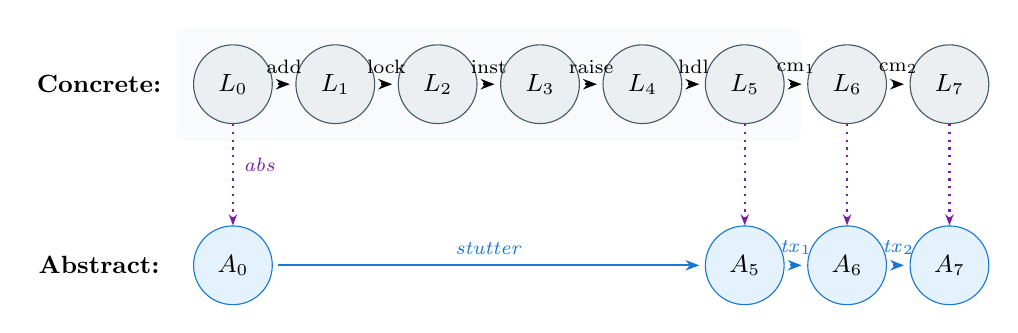
\begin{tikzpicture}[
  cstate/.style={draw, circle, minimum size=1.0cm, font=\small, fill=palGrayLt, draw=palGray},
  astate/.style={draw, circle, minimum size=1.0cm, font=\small, fill=palBlueLt, draw=palBlue},
  >=Stealth,
  node distance=1.2cm
]
\def\yConcrete{1.5}    % y-position for concrete row
\def\yAbstract{-0.8}   % y-position for abstract row
\def\xSpacing{1.3}     % horizontal spacing between concrete states

%% Concrete Row
\node[font=\small\bfseries] at (-1.7, \yConcrete) {Concrete:};
\foreach \i/\lbl in {0/L_0, 1/L_1, 2/L_2, 3/L_3, 4/L_4, 5/L_5, 6/L_6, 7/L_7} {
  \node[cstate] (c\i) at (\i*\xSpacing, \yConcrete) {$\lbl$};
}

%% Concrete Edges
\foreach \i/\j/\lbl in {0/1/add,1/2/lock,2/3/inst,3/4/raise,4/5/hdl,5/6/cm$_1$,6/7/cm$_2$} {
  \draw[stdarrow] (c\i) -- node[above, font=\scriptsize] {\lbl} (c\j);
}

%% Stuttering Background
\begin{scope}[on background layer]
  \node[rounded corners, fill=palGrayLt!30, fit=(c0)(c5), inner sep=6pt] {};
\end{scope}

%% Abstract Row — aligned to concrete node x-positions
\node[font=\small\bfseries] at (-1.7, \yAbstract) {Abstract:};
\node[astate] (a0) at (c0 |- 0,\yAbstract) {$A_0$};
\node[astate] (a5) at (c5 |- 0,\yAbstract) {$A_5$};
\node[astate] (a6) at (c6 |- 0,\yAbstract) {$A_6$};
\node[astate] (a7) at (c7 |- 0,\yAbstract) {$A_7$};

%% Abstract Edges
\draw[stdarrow, palBlue] (a0) -- node[above, font=\scriptsize] {$\mathit{stutter}$} (a5);
\draw[stdarrow, palBlue] (a5) -- node[above, font=\scriptsize] {$\mathit{tx}_1$} (a6);
\draw[stdarrow, palBlue] (a6) -- node[above, font=\scriptsize] {$\mathit{tx}_2$} (a7);

%% Abstraction Map
\draw[stutterarrow, palPurple] (c0) -- node[right, font=\scriptsize, pos=0.4] {$\mathit{abs}$} (a0);
\draw[stutterarrow, palPurple] (c5) -- (a5);
\draw[stutterarrow, palPurple] (c6) -- (a6);
\draw[stutterarrow, palPurple] (c7) -- (a7);
\end{tikzpicture}
\caption{Refinement diagram: concrete concurrent steps map to abstract serial steps via $\mathit{absLedger}$. Non-commit steps are stuttering.}
\label{fig:refinement}
\end{figure}

\begin{theorem}[Circuit Witness Implies Serial Step]\label{thm:circuit-serial}
$\mathit{refinementWitness}(m, L, \mathit{tx}) \implies \mathit{SerialStep}(m, L, \mathit{applyCommit}(L, \mathit{tx}))$, where $\mathit{refinementWitness}$ is $\mathit{coordCommitEnabled}$ restricted to a single transaction.
\emph{(Mechanized: \texttt{circuit\_witness\_implies\_serial\_step}.)}
\end{theorem}

Together, the bridge results give a two-level guarantee: serializable histories (\cref{sec:serializability}) and faithful protocol implementation, under the security assumptions of \cref{sec:state-components}.

%% ═══════════════════════════════════════════════════════════════════════════
\section{Formal Verification}\label{sec:mechanization}

The ICE-UTxO model is verified through two complementary formal artifacts: a Lean~4 mechanization that proves safety properties universally, and a TLA+ specification that validates liveness properties by model checking under fairness assumptions. Neither artifact alone covers the full verification space; together, they do.

\subsection{Dual Verification Strategy}\label{sec:dual-strategy}

Safety properties guarantee that the system never enters an invalid state, but a ledger that commits nothing satisfies all of them. ICE-UTxO introduces three liveness risks absent from vanilla eUTxO: lock starvation (pessimistic mode), coroutine deadlock (stalled effect queues), and cross-shard progress failure (S-BAC consensus stalls). Lean cannot express temporal operators ($\Box$, $\Diamond$, $\mathit{WF}$); TLA+ can express liveness but validates only on bounded instances. The relationship is symbiotic: Lean proves \emph{enabling conditions} (commit is available, abort is always possible, effect handling decreases the queue); TLA+ validates that fair scheduling eventually \emph{exploits} those conditions.

\subsection{Lean Proof Architecture}\label{sec:mech-architecture}

The development follows a two-track architecture connected by a bridge, reflecting a real separation between two proof domains. Track~1 (Ledger) reasons about UTxO state, conflicts, and serializability; Track~2 (Coordination) reasons about event structures, projections, and protocol compliance. The two tracks share a narrow interface --- the $\mathit{coordCommitEnabled}$ predicate. The only classical reasoning is three \texttt{by\_contra} case splits on decidable propositions.

\paragraph{Track~1 (Ledger).}
Central objects: \texttt{Step} (8 constructors), $\mathit{ledgerInvariant}$ (6-part safety predicate), $\mathit{CoreState}$ (abstraction enabling commutativity), and $\mathit{absLedger}$ (refinement map). The design relies on a double abstraction: $\mathit{CoreState}$ drops history for serializability; $\mathit{absLedger}$ drops concurrency-control fields for stuttering simulation.

\paragraph{Track~2 (Coordination).}
Central objects: \texttt{Script} (event structure), \texttt{LocalScript} (per-role projection), \texttt{Program} (PTB commands combining into $\mathit{orderRel}$ and $\mathit{conflictRel}$), and \texttt{CoordWitness} (script--trace pair). Global trace consistency decomposes into per-role local conformance plus cross-role consistency.

\paragraph{The bridge.}
The predicate $\mathit{coordCommitEnabled}$ conjoins $\mathit{commitEnabledStrong}$ (ledger guard) and $\mathit{witnessGlobalOK}$ (coordination guard). The bridge theorems show this conjunction decomposes to shard-local checks.

\paragraph{The Oracle subtrack.}
An independent executable model (\texttt{Starstream/Oracle/*.lean}) uses \texttt{Bool}-valued predicates and gas metering. PhaseD bridge theorems lift key properties to the Oracle namespace, each requiring only a single \texttt{simpa~using} tactic, confirming no new proof obligations.

\begin{figure}[t]
\centering
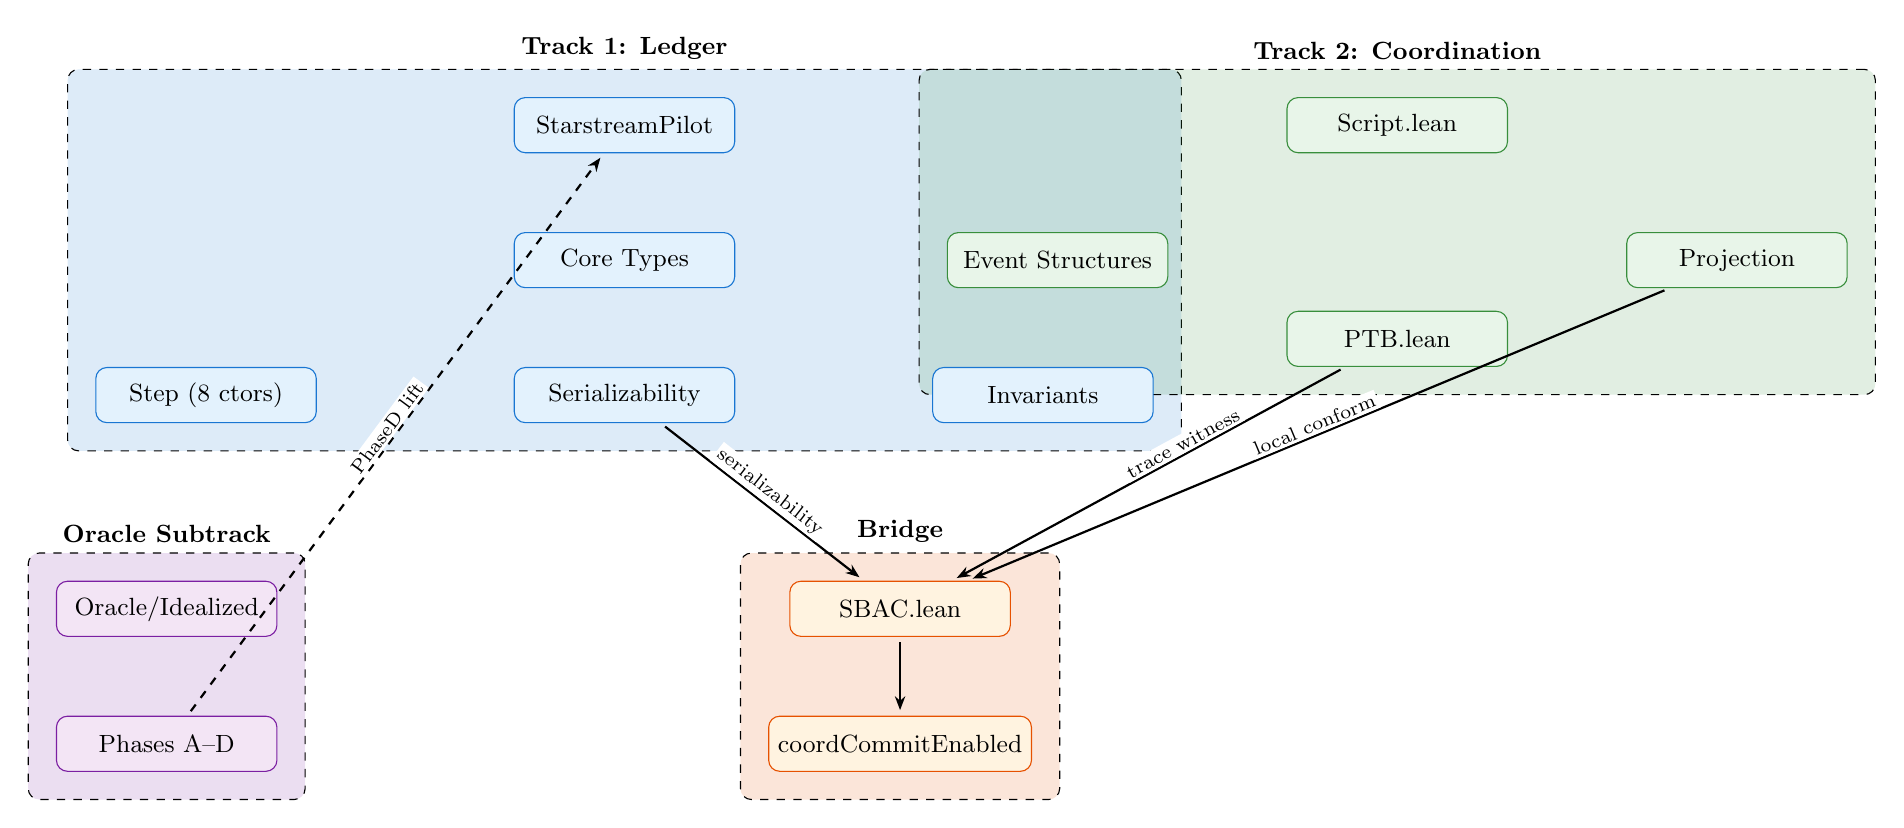
\begin{tikzpicture}[
  mnode/.style={modnode, minimum width=2.8cm},
  >=Stealth,
  node distance=1.0cm
]
%% Track 1: Ledger
\node[mnode, fill=palBlueLt, draw=palBlue] (ssp) {StarstreamPilot};
\node[mnode, fill=palBlueLt, draw=palBlue, below=of ssp] (core) {Core Types};
\node[mnode, fill=palBlueLt, draw=palBlue, below left=1.0cm and 2.5cm of core] (step) {Step (8 ctors)};
\node[mnode, fill=palBlueLt, draw=palBlue, below=of core] (serial) {Serializability};
\node[mnode, fill=palBlueLt, draw=palBlue, below right=1.0cm and 2.5cm of core] (inv) {Invariants};
\begin{scope}[on background layer]
  \node[trackgroup, fill=palBlue, label={[font=\small\bfseries]above:Track 1: Ledger}]
    (t1bg) [fit=(ssp)(core)(step)(serial)(inv)] {};
\end{scope}

%% Track 2: Coordination
\node[mnode, fill=palGreenLt, draw=palGreen, right=7.0cm of ssp] (script) {Script.lean};
\node[mnode, fill=palGreenLt, draw=palGreen, below left=1.0cm and 1.5cm of script] (es) {Event Structures};
\node[mnode, fill=palGreenLt, draw=palGreen, below right=1.0cm and 1.5cm of script] (proj) {Projection};
\node[mnode, fill=palGreenLt, draw=palGreen, below=2.0cm of script] (ptb) {PTB.lean};
\begin{scope}[on background layer]
  \node[trackgroup, fill=palGreen, label={[font=\small\bfseries]above:Track 2: Coordination}]
    [fit=(script)(es)(proj)(ptb)] {};
\end{scope}

%% Bridge
\node[mnode, fill=palOrangeLt, draw=palOrange, below=2.0cm of serial, xshift=3.5cm] (sbac) {SBAC.lean};
\node[mnode, fill=palOrangeLt, draw=palOrange, minimum width=3.2cm, below=of sbac] (coord) {coordCommitEnabled};
\begin{scope}[on background layer]
  \node[trackgroup, fill=palOrange, label={[font=\small\bfseries]above:Bridge}]
    [fit=(sbac)(coord)] {};
\end{scope}

%% Oracle Subtrack
\node[mnode, fill=palPurpleLt, draw=palPurple, below=2.0cm of step, xshift=-0.5cm] (oracle) {Oracle/Idealized};
\node[mnode, fill=palPurpleLt, draw=palPurple, below=of oracle] (phases) {Phases A--D};
\begin{scope}[on background layer]
  \node[trackgroup, fill=palPurple, label={[font=\small\bfseries]above:Oracle Subtrack}]
    [fit=(oracle)(phases)] {};
\end{scope}

%% Dependency Edges
\draw[stdarrow] (serial) -- node[above, font=\scriptsize, sloped, fill=white, inner sep=1pt] {serializability} (sbac);
\draw[stdarrow] (ptb) -- node[above, font=\scriptsize, sloped, fill=white, inner sep=1pt, pos=0.4] {trace witness} (sbac);
\draw[stdarrow] (proj) -- node[above, font=\scriptsize, sloped, fill=white, inner sep=1pt] {local conform} (sbac);
\draw[stdarrow] (sbac) -- (coord);
\draw[stdarrow, dashed] (phases) -- (ssp) node[midway, above, font=\scriptsize, sloped, fill=white, inner sep=1pt] {PhaseD lift};
\end{tikzpicture}
\caption{Proof architecture of the Lean mechanization. The two tracks meet at $\mathit{coordCommitEnabled}$ through the SBAC bridge. The Oracle subtrack connects back to Track~1 via PhaseD bridge theorems.}
\label{fig:module-deps}
\end{figure}

\subsection{What Is Proved}\label{sec:what-is-proved}

The mechanization establishes three main results connected by a bridge. (1)~$\mathit{step\_preserves\_invariant}$ proves invariant preservation for all \texttt{Step} constructors; $\mathit{init\_ledgerInvariant}$ and $\mathit{ledgerInvariant\_steps}$ lift this to initial states and multi-step executions. (2)~$\mathit{core\_commute}$ and $\mathit{acyclic\_strong\_serializable}$ establish conflict serializability (\cref{sec:bubble-sort}). (3)~$\mathit{concurrent\_refines\_serial}$ classifies seven of eight steps as stuttering (\cref{sec:refinement}). The bidirectional witness theorems (\cref{thm:bidirectional}) decompose global protocol checking into shard-local checks; $\mathit{commit\_requires\_proof}$ shows only proof-verified transactions extend history; $\mathit{consumed\_monotone\_step}$ establishes asset finality. \Cref{tab:theorems} provides a compact reference.

\begin{table}[t]
\caption{Principal theorems in the Lean mechanization.}
\label{tab:theorems}
\centering\small
\begin{tabular}{llll}
\toprule
\textbf{Theorem} & \textbf{File} & \textbf{Statement (informal)} & \textbf{Technique} \\
\midrule
\texttt{core\_commute} & StarstreamPilot & Non-conflicting txs commute at CoreState & Finset extensionality \\
\texttt{acyclic\_strong\_serializable} & StarstreamPilot & Acyclic $\Rightarrow$ all conflict-respecting perms agree & Bubble-sort induction \\
\texttt{commit\_requires\_proof} & StarstreamPilot & Only proof-verified txs extend history & 8-way case analysis \\
\texttt{step\_preserves\_invariant} & StarstreamPilot & Every Step preserves 6-part invariant & Floyd--Hoare analysis \\
\texttt{concurrent\_refines\_serial} & StarstreamPilot & Concurrent refines serial via stuttering & Stuttering simulation \\
\texttt{proj\_localConform\_of\_globalConform} & Script & Global conformance $\Rightarrow$ local conformance & Structural induction \\
\texttt{traceConsistent\_of\_local\_and\_cross} & Script & Local + cross-role $\Rightarrow$ global consistency & Decidable case split \\
\texttt{toScript\_wellFormed} & PTB & PTB programs produce well-formed scripts & 7-way decomposition \\
\texttt{witnessLocalOK\_of\_global} & SBAC & Global witness $\Rightarrow$ local witness & Projection \\
\texttt{witnessGlobalOK\_of\_local\_and\_consistent} & SBAC & Consistent local $\Rightarrow$ global & Consistency theorem \\
\texttt{coordCommitEnabledLocal\_of\_global} & SBAC & Global commit $\Rightarrow$ all-local commit & Decomposition \\
\bottomrule
\end{tabular}
\end{table}

\subsection{TLA+ Specification and Validation}\label{sec:tla-architecture}

The TLA+ specification comprises 20~modules (${\sim}5{,}100$~lines) in five layers, defining two behavioral state machines---\texttt{StarstreamSpec} (pessimistic) and \texttt{StarstreamSpecOptimistic} (snapshot-based)---both model-checked against a shared invariant framework. A serial abstraction (\texttt{StarstreamSerial}) defines atomic commit; the refinement module classifies 14 of 20+ actions as stuttering and states $\mathit{Spec} \Rightarrow \mathit{SerialSpec}$.

\paragraph{Liveness properties.}
Four liveness properties address progress risks specific to ICE-UTxO. \Cref{tab:liveness} summarizes them.

\begin{table}[t]
\caption{TLA+ liveness properties and their relationship to Lean safety lemmas.}
\label{tab:liveness}
\centering\small
\begin{tabular}{lp{3.5cm}lp{2.5cm}}
\toprule
\textbf{Property} & \textbf{Prevents} & \textbf{Lean lemma} & \textbf{Fairness} \\
\midrule
L1: Eventual commit & Throughput failure & \texttt{commit\_step\_specific} & $\mathit{WF}(\text{commit})$ \\
L2: Eventual termination & Lock starvation & \texttt{abort\_enabled\_of\_pending} & $\mathit{WF}(\text{abort})$ \\
L3: Effect handling & Coroutine deadlock & \texttt{handleEffect\_decreases\_effects} & $\mathit{WF}(\text{handleE})$ \\
L4: Return to idle & Unbounded pending work & (compositional) & Fair role participation \\
\bottomrule
\end{tabular}
\end{table}

L1 ($\Diamond\Box\,\mathit{CommitEnabled} \Rightarrow \Diamond\,\mathit{Committed}$) prevents throughput stalls. L2 ($\Box(\mathit{Pending} \Rightarrow \Diamond\,\neg\mathit{Pending})$) prevents lock starvation. L3 ($\mathit{HasEffects} \leadsto \mathit{EffectsCleared}$) prevents coroutine deadlock; the Lean descent lemma provides the well-founded argument, TLA+ validates that fair scheduling completes it. L4 ($\Box\Diamond(\mathit{pendingTxs} = \{\})$) ensures work does not accumulate without bound.

\paragraph{Safety invariants.}
The specification checks 47~named invariants in twelve categories (\cref{tab:tla-invariants}). These decompose finer-grained concerns implicit in Lean's six-part $\mathit{ledgerInvariant}$. For instance, Lean's $\mathit{noDoubleSpend}$ corresponds to four separate TLA+ linearity invariants, each independently model-checked.

\begin{table}[t]
\caption{TLA+ safety invariant categories.}
\label{tab:tla-invariants}
\centering\small
\begin{tabular}{lrl}
\toprule
\textbf{Category} & \textbf{Count} & \textbf{Protects} \\
\midrule
Type safety & 5 & Well-formed ledger, frames, token bags \\
Authorization & 2 & Valid signatures, owner-only spending \\
Balance & 4 & Token conservation, NFT uniqueness, overflow \\
Linearity & 6 & No double-spend, consumed tracking, unique IDs \\
IEUTxO/chunk & 7 & Transaction sequence validity, proof gating \\
Locking & 4 & Exclusive locks, consistent reservation \\
Optimistic & 4 & Read-set/write-set consistency, snapshot isolation \\
Lifecycle & 3 & Consumed finality, frame--state consistency \\
Effects & 10 & Handler matching, orphan freedom, stack bounds \\
Proofs & 8 & IVC integrity, phase consistency, no double proof \\
Circuit alignment & 8 & Dual-trace consistency, activation, value commitment \\
Attack/rollback & 4 & No replay, ID monotonicity, no output leaks \\
\bottomrule
\end{tabular}
\end{table}

\paragraph{Circuit-to-specification alignment.}
The \texttt{StarstreamCircuitAlignment} module connects the ZK circuit to the specification via three mapping tables and eight circuit-specific invariants. A gap analysis identifies seven property categories requiring ledger-level validation (optimistic concurrency, token balance, authorization, liveness, read-set validation, NFT uniqueness, rollback safety), decomposing Lean's single oracle into $\mathit{CircuitVerifiable}$, $\mathit{RequiresLedgerValidation}$, and $\mathit{FullyVerified}$.

\paragraph{Adversarial modeling.}
The specification includes adversarial actions ($\mathit{InjectInvalidTx}$, $\mathit{RejectInvalidTx}$). Model checking confirms that no action sequence, including adversarial injection, violates any of the 47~safety invariants.

\subsection{Cross-Artifact Traceability}\label{sec:cross-artifact}

The Lean and TLA+ artifacts are cross-referenced at three levels: liveness-to-safety dependencies, shared concepts, and corresponding theorems. \Cref{tab:cross-artifact} summarizes the principal correspondences.

\begin{table}[t]
\caption{Cross-artifact traceability between Lean proofs and TLA+ specification.}
\label{tab:cross-artifact}
\centering\small
\begin{tabular}{lll}
\toprule
\textbf{TLA+ artifact} & \textbf{Lean artifact} & \textbf{Relationship} \\
\midrule
$\mathit{SerialRefinement}$ & $\mathit{concurrent\_refines\_serial}$ & Behavioral vs. relational \\
$\mathit{INV\_CIRCUIT\_*}$ (8) & $\mathit{commit\_requires\_proof}$ & Internal structure vs. oracle \\
$\mathit{LIVE\_TxEventuallyTerminates}$ & $\mathit{abort\_enabled\_of\_pending}$ & Temporal conclusion vs. enabling \\
$\mathit{LIVE\_EffectsEventuallyHandled}$ & $\mathit{handleEffect\_decreases\_effects}$ & Fair scheduling vs. descent \\
$\mathit{INV\_Safety}$ (47) & $\mathit{ledgerInvariant}$ (6-part) & Fine-grained vs. compositional \\
$\mathit{coordCommitEnabled}$ & $\mathit{coordCommitEnabled}$ & Shared predicate \\
20+ actions & 8 \texttt{Step} constructors & Behavioral vs. relational \\
\bottomrule
\end{tabular}
\end{table}

Lean proves universal properties ($\forall$ states, $\forall$ steps) over unbounded state spaces; TLA+ validates temporal properties ($\Box$, $\Diamond$, $\mathit{WF}$) on bounded instances. The eight TLA+ circuit alignment invariants provide the internal structure that Lean's verifier oracle abstracts away.

\Cref{tab:coverage} shows property coverage. The TLA+ refinement claim ($\mathit{Spec} \Rightarrow \mathit{SerialSpec}$) is stated but not TLC-verified; the implication requires a refinement-mapping proof in TLAPS.

\begin{table}[t]
\caption{Property coverage across formal artifacts.}
\label{tab:coverage}
\centering\small
\begin{tabular}{lccp{4.8cm}}
\toprule
\textbf{Property} & \textbf{Lean} & \textbf{TLA+} & \textbf{Notes} \\
\midrule
No double-spend              & $\checkmark$ & $\checkmark$ & Lean: part of 6-part invariant; TLA+: 4 linearity invariants \\
Conflict serializability     & $\checkmark$ &              & Universal, constructive \\
Concurrent-to-serial refine. & $\checkmark$ & stated       & TLA+ states $\mathit{Spec} \Rightarrow \mathit{SerialSpec}$; not TLC-verified \\
Proof-gated commit           & $\checkmark$ & $\checkmark$ & Lean: oracle; TLA+: 8 circuit invariants \\
Invariant preservation       & $\checkmark$ & $\checkmark$ & Lean: 6-part; TLA+: 47 named \\
MPST decomposition           & $\checkmark$ &              & Bidirectional bridge \\
PTB well-formedness          & $\checkmark$ &              & \\
Eventual commit (L1)         &              & $\checkmark$ & Lean supplies enabling lemma \\
Eventual termination (L2)    &              & $\checkmark$ & Lean supplies enabling lemma \\
Effect handling (L3)         &              & $\checkmark$ & Lean supplies descent lemma \\
Return to idle (L4)          &              & $\checkmark$ & Compositional \\
Handler-stack consistency    &              & $\checkmark$ & \texttt{GuardUninstallHandler}; absent from Lean \\
Circuit alignment            &              & $\checkmark$ & 8 invariants, 12 op mappings \\
\bottomrule
\end{tabular}
\end{table}

\subsection{How the Proofs Work}\label{sec:proof-techniques}

\paragraph{Proof techniques.}
Serializability: strong induction on history length via \texttt{List.reverseRecOn} (\cref{sec:bubble-sort}). Invariant preservation: eight-way case analysis on \texttt{Step} constructors; only \texttt{commit} modifies UTxOs, consumed, and history simultaneously. Refinement: per-constructor stuttering lemmas showing $\mathit{absLedger}(L) = \mathit{absLedger}(L')$ for seven of eight cases. Coordination: shared-role/disjoint-role case split.

\subsection{Lessons Learned}\label{sec:lessons}

\paragraph{Constructivity and axiom discipline.}
A single \texttt{by\_cases} invocation (Script.lean, line~643) performs a decidable case split on finite role sets; everything else is constructive. The bubble-sort proof constructs the transposition sequence explicitly. Only standard Mathlib axioms (propext, Quot.sound, funext) are in scope.

\paragraph{The identity-permutation false start.}
The initial \texttt{coreSerializable} was proved with the identity permutation---technically correct but vacuous. The corrected \texttt{strongCoreSerializable} universally quantifies over all conflict-respecting permutations. Lean checked both without complaint; only adversarial review of the \emph{statement} caught the error. Type-checkers guarantee proof correctness, not statement adequacy.

\paragraph{The two-track decomposition as a proof management strategy.}
Changes to event-structure semantics never required re-checking ledger proofs, and vice versa. The narrow interface (\texttt{CoordTx} type and \texttt{coordCommitEnabled}) made iterative development practical: serializability was reworked three times without touching coordination.

\paragraph{The Oracle as a specification testbed.}
The Oracle subtrack's \texttt{Bool}-valued predicates exposed specification bugs that \texttt{Prop}-valued predicates could not, since counterexamples were computable. PhaseD bridge theorems confirmed every Oracle property lifts to the protocol layer with a single \texttt{simpa~using} per theorem.

\paragraph{Complementary mechanizations.}
Tirore et al.~\cite{Tirore2025} provide the first mechanized proof of subject reduction for MPST in Coq; their work is complementary to ours and could serve as a certified front-end for session-type checking feeding into ICE-UTxO's ledger-level back-end.

\paragraph{TLA+ as a specification review tool.}
The TLA+ specification exposed implicit assumptions in the Lean development. The circuit alignment module's gap analysis revealed seven categories of properties outside the circuit's scope. Model checking caught a handler-stack consistency bug: uninstalling a handler while an effect was pending led to an orphaned effect, prompting the $\mathit{GuardUninstallHandler}$ precondition. This guard is present in TLA+ but absent from Lean's \texttt{Step.uninstallH} (a known gap; adding it to Lean is planned).

\subsection{Trust Boundaries}\label{sec:trust-boundaries}

Three trust-boundary assumptions are marked in the source code (F3, F5, F9). \textbf{F3}: $\mathit{allProofsVerified}$ is an oracle---every safety theorem is conditional on ZK verifier soundness. \textbf{F5}: $\mathit{readSetValid}$ is a pure existence check, sufficient for snapshot consistency because UTxOs are immutable from creation to consumption. \textbf{F9}: $\mathit{handleEffect}$ returns $\mathit{none}$ when no handler is installed; the event-structure causal order guarantees $\mathit{installH}$ precedes $\mathit{handleE}$.

The irreducible external assumptions (\cref{sec:commit-rule,sec:bridge}) are: (i)~IVC/SNARK soundness, (ii)~S-BAC shard honesty ($f < n/3$ per shard~\cite{AlBassam2018}), and (iii)~weak fairness for commit and abort actions. Every safety theorem is conditional on~(i); every liveness claim on~(ii) and~(iii).

\subsection{Limitations}\label{sec:limitations}

\begin{enumerate}
  \item \textbf{ZK verifier is an oracle.} Every safety theorem is conditional on verifier soundness; breaking the verifier breaks the trust chain.

  \item \textbf{Phase ordering is not statically enforced.} The \texttt{Step} constructors do not prevent out-of-order firing. An indexed inductive family parameterized by phase would close this gap.

  \item \textbf{Liveness is argued, not proved.} Supporting lemmas are mechanized (\texttt{pending\_can\_step}, effect queue descent), but temporal conclusions require fairness assumptions outside Lean's logic. TLC validates on bounded instances.

  \item \textbf{S-BAC is a specification, not a verified implementation.} \texttt{SBAC.lean} defines logical predicates and proves bidirectional theorems but does not model message passing or BFT. Mechanizing this layer (e.g., via Verdi~\cite{Wilcox2015}) would close the gap.

  \item \textbf{No programming-language semantics.} The model formalizes scripts and traces but not the coroutine calculus or effect-handler operational semantics.

  \item \textbf{All identifiers are \texttt{Nat}.} Type distinction between UTXOId, TxId, etc.\ is collapsed. Proofs remain sound but the specification is weaker against modeling errors.

  \item \textbf{TLA+ covers only bounded instances.} Refinement theorems are stated but not mechanically proved; they require TLAPS.
\end{enumerate}

%% ═══════════════════════════════════════════════════════════════════════════
\section{Related Work}\label{sec:related}

ICE-UTxO sits at the intersection of multiparty session types, UTxO-based blockchain models, sharded consensus, and mechanized verification of concurrent systems. We organise the related literature along these four axes, devoting the most space to session-type theory, which is closest to our contribution. \Cref{tab:novelty} summarizes the relationship between each ICE-UTxO component and its prior art.

\begin{table}[t]
\caption{Novelty positioning: each ICE-UTxO component, its prior art, and what is specifically new.}
\label{tab:novelty}
\centering\small
\begin{tabular}{p{2.8cm}p{4.5cm}p{5.5cm}}
\toprule
\textbf{Component} & \textbf{Prior Art} & \textbf{ICE-UTxO Contribution} \\
\midrule
Coroutine frames on UTxOs & Ergo multi-stage contracts~\cite{Chepurnoy2019}; Sui PTBs~\cite{Blackshear2023} & Atomic intra-transaction interleaving of multiple UTXO scripts with saved frame state $(pc, locals, methodId, hash)$ within the eUTxO model \\
\addlinespace
Algebraic effects & Plotkin \& Pretnar~\cite{PlotkinPretnar2009} in PL theory & First application of full algebraic effects (raise/handle/resume) to on-chain UTXO validators, with dynamically-scoped handlers bounded by transaction scope \\
\addlinespace
MPST coordination & Honda et al.~\cite{Honda2016}; Nomos~\cite{Das2021} for binary session types in smart contracts & Extension to multiparty global types with event-structure semantics, projected to per-role local types verified at ledger submission time \\
\addlinespace
PTB compilation & Sui PTBs~\cite{Blackshear2023} & Formal compilation from MPST global types to PTB-style bytecode with mechanized correctness proofs \\
\addlinespace
IVC proof-gating & ZEXE~\cite{Bowe2018}/Aleo~\cite{Aleo2021} for proof-carrying txs; Nova~\cite{Kothapalli2022}/HyperNova~\cite{Kothapalli2023} for IVC & Proofs certify multiparty protocol compliance (session fidelity), not just arbitrary computation or privacy \\
\addlinespace
S-BAC cross-shard & Chainspace~\cite{AlBassam2018}; OmniLedger~\cite{KokorisKogias2018} & Composition of S-BAC with session-type witness verification, enforcing protocol structure as well as ledger invariants \\
\bottomrule
\end{tabular}
\end{table}

\subsection{Multiparty Session Types}

\paragraph{Foundational theory.}
The multiparty session type (MPST) discipline originates with Honda, Yoshida, and Carbone~\cite{Honda2016}, who introduced \emph{global types} as choreographic specifications from which local endpoint types are obtained by \emph{projection}. Their framework guarantees communication safety, session fidelity, and progress for asynchronous sessions with arbitrarily many participants. ICE-UTxO adopts the global-type/projection architecture wholesale but departs in two critical ways: (i)~our global types are indexed by \emph{UTxO references} rather than channel names, so that each protocol step is anchored to an on-chain datum; and (ii)~projection targets \emph{transaction validator scripts} rather than process calculi, yielding proof obligations that are discharged at ledger-submission time rather than at compile time.

H\"{u}ttel et al.~\cite{Huttel2016} survey session types and behavioural contracts, classifying systems by their type discipline, communication medium, and verification strategy. In the taxonomy they propose, ICE-UTxO occupies an unoccupied cell: it is an \emph{asynchronous, event-structure-based} system whose communication medium is a \emph{shared ledger} rather than point-to-point channels or shared memory.

\paragraph{Interleaving and global progress.}
Bettini et al.~\cite{Bettini2008} study \emph{global progress} for multiparty sessions that are dynamically interleaved on shared channels. Their finding is that progress requires not only local typing but also a global ordering condition on channel usage. Coppo et al.~\cite{Coppo2013,Coppo2016} subsequently show that this ordering can be \emph{inferred} rather than annotated, using a constraint-based analysis.

ICE-UTxO faces a structurally analogous problem: multiple protocol instances may share UTxO outputs, creating potential deadlocks at the ledger level. Our solution encodes the global ordering directly in the \emph{event-structure causal order} (\cref{sec:model}) and enforces it via S-BAC lock acquisition (\cref{sec:bridge}). The difference is that in our setting the ``channels'' are UTxO cells whose consumption is \emph{atomic and irrevocable}, which simplifies the progress argument but introduces the need for cross-shard coordination that classical MPST avoids.

\paragraph{Beyond duality.}
Scalas and Yoshida~\cite{Scalas2019} generalise binary session types beyond syntactic duality using a \emph{rely/guarantee} formulation inspired by concurrent separation logic. ICE-UTxO draws on this philosophy when it decomposes a global protocol into per-validator proof obligations (\cref{sec:event-structure-semantics}): each validator's correctness proof \emph{relies} on the structural guarantees of the UTxO model (uniqueness of consumption) and \emph{guarantees} local adherence to the projected session type. Our setting is inherently multiparty, however, so the rely/guarantee decomposition is driven by projection from a global type rather than by binary co-typing.

\paragraph{Event-structure semantics.}
Castellani, Dezani-Ciancaglini, and Giannini~\cite{Castellani2023} develop an \emph{event-structure semantics} for asynchronous multiparty session types, replacing the traditional operational semantics based on labelled transition systems with a denotational model in which communication actions are events related by causality and conflict. This is closely related work to ours. Their event structures capture the true concurrency inherent in asynchronous multiparty interaction, avoiding the artificial interleaving that LTS-based semantics impose.

ICE-UTxO builds directly on this line of work. Our \emph{transaction event structures} (\cref{sec:model}) instantiate the Castellani--Dezani-Ciancaglini--Giannini framework in a blockchain setting: events are ledger transitions, causality is the UTxO spend relation, and conflict arises when two transactions attempt to consume the same output. We extend their model in three ways: (i)~we add \emph{algebraic effects} to events, allowing each transaction to carry computational side-effects interpreted by the ledger runtime; (ii)~we annotate events with \emph{proof witnesses}, transforming the event structure into a \emph{proof-carrying} artefact; and (iii)~we provide a \emph{mechanised} (Lean~4) equivalence proof between the event-structure semantics and the operational semantics, whereas Castellani et al.'s results are paper-based.

\paragraph{Monitoring and hybrid verification.}
Bocchi et al.~\cite{Bocchi2017} introduce \emph{monitors} derived from multiparty session types for verifying communication at runtime. Neykova et al.~\cite{Neykova2017} extend this approach to \emph{timed} multiparty sessions. ICE-UTxO adopts a conceptually similar runtime-verification architecture, but the ``monitor'' is the ledger's transaction-validation logic itself. Each transaction carries a proof witness checked by the validator script before admission to the chain, providing \emph{enforcement} rather than mere detection.

Hu and Yoshida~\cite{Hu2016} propose \emph{hybrid session verification}, combining static typing of the protocol skeleton with runtime checking of data-dependent branching. ICE-UTxO follows a broadly similar hybrid strategy: the \emph{structural} properties of the protocol (ordering, participation, branching topology) are verified statically by our Lean~4 metatheory, while \emph{payload} properties (datum validity, value conservation) are checked dynamically by on-chain validators using proof-carrying witnesses.

\paragraph{Tooling and code generation.}
The \emph{Scribble} protocol description language~\cite{Yoshida2014} provides a practical surface syntax for global types. \emph{NuScr}~\cite{Zhou2021} extends Scribble with a CFSM-based backend supporting automated protocol validation and endpoint code generation. ICE-UTxO's protocol description layer (\cref{sec:model}) is inspired by Scribble's design but targets a different backend: instead of generating communicating finite-state machines, our compilation pipeline produces PTB-style programs with formally verified correctness properties (\cref{sec:ptb-compilation}).

Voinea et al.~\cite{Voinea2020} present \emph{StMungo}, translating Scribble protocols into typestate specifications for Java. King et al.~\cite{King2019} apply MPST to web development with static linearity. Miu et al.~\cite{Miu2021cc,Miu2020places} extend this line to TypeScript with WebSocket code generation. These tools demonstrate the practical viability of MPST-based code generation. ICE-UTxO contributes to this tradition by targeting \emph{blockchain validator scripts}---a domain where code-generation correctness is especially critical because deployed validators cannot be patched and govern the movement of real assets.

\paragraph{Session types for smart contracts.}
Das, Balzer, Hoffmann, and Pfenning~\cite{Das2021} introduced the Nomos system, which is the most directly relevant prior work applying session types to smart contract programming. Nomos uses binary session types grounded in intuitionistic linear logic to ensure that digital contracts satisfy resource-linearity properties: tokens cannot be duplicated or destroyed outside of explicitly authorized operations. Nomos contracts communicate via typed channels, and the type system statically guarantees that all protocol interactions conform to their session type specifications. However, Nomos differs from ICE-UTxO in several important respects. First, the original Nomos system uses binary (two-party) session types; subsequent work by Das and Pfenning~\cite{DasPfenning2022} introduces shared session types that allow multiple clients to interact with a shared contract, but the underlying type discipline remains two-party at the session level. ICE-UTxO uses multiparty session types with arbitrarily many roles---a distinction that matters for protocols involving more than two participants (e.g., the collateralized loan scenario with oracle, borrower, liquidator, and coordinator). Second, Nomos operates within its own custom contract language and runtime, while ICE-UTxO extends the existing eUTxO model and targets existing Plutus-style validators. Third, Nomos verifies protocol adherence at compile time through its type system, while ICE-UTxO verifies protocol adherence at ledger submission time through IVC proof witnesses---a design choice driven by the open, permissionless nature of blockchain systems where contract code may come from untrusted sources. ICE-UTxO can be viewed as extending the Nomos vision from binary to multiparty, from a custom runtime to the eUTxO ledger, and from static type checking to dynamic proof-carrying verification.

\paragraph{Adaptation and replication.}
Harvey et al.~\cite{Harvey2021} introduce \emph{connection actions} that allow sessions to adapt at runtime by adding or removing participants. ICE-UTxO supports a limited form of adaptation through its \emph{coroutine suspension} mechanism: a participant may suspend, allowing another party to resume in a later transaction. However, we do not currently support arbitrary participant addition or removal.

Le~Brun et al.~\cite{LeBrun2025} extend MPST with \emph{replication}, enabling protocols that spawn unboundedly many sub-sessions. This is relevant because blockchain protocols often involve unbounded repetition (e.g., a payment channel processing arbitrarily many off-chain updates). Our current formalisation handles bounded unfolding; incorporating replication is future work.

Tirore et al.~\cite{Tirore2025} provide the first \emph{mechanised} proof of subject reduction for MPST, formalised in Coq. ICE-UTxO shares this commitment to mechanised metatheory but targets \emph{ledger-level safety and progress} rather than subject reduction for a process calculus, and is carried out in Lean~4 rather than Coq. We view the two as complementary: their mechanised subject reduction could serve as a certified front-end feeding into our ledger-level back-end.

\subsection{UTxO Models and Blockchain Verification}

The UTxO model was introduced with Bitcoin~\cite{Nakamoto2008}, where each transaction consumes outputs produced by previous transactions and creates new ones. Bitcoin's scripting language is intentionally limited, making transactions easy to validate in parallel---a property ICE-UTxO inherits---but precludes the expression of complex multi-step protocols.

Chakravarty et al.~\cite{Chakravarty2020} introduce the \emph{extended UTxO} (eUTxO) model underlying Cardano. eUTxO enriches Bitcoin's model with \emph{datums} and \emph{validator scripts}. ICE-UTxO extends eUTxO in three directions: (i)~we add \emph{coroutine state} to datums, enabling multi-step protocols encoded as suspended computations; (ii)~we introduce \emph{algebraic effects} into the validator execution model; and (iii)~we require each transaction to carry a \emph{proof witness} demonstrating conformance to a projected session type.

Melkonian et al.~\cite{Melkonian2019} provide a mechanically verified reference semantics for the Cardano ledger in Agda. P\^{i}rlea and Sergey~\cite{PirleaSergey2023} mechanize blockchain consensus properties in Coq. Park et al.~\cite{Park2018} provide formal verification tools for Ethereum VM bytecode. ICE-UTxO's Lean~4 formalisation covers analogous ground to Melkonian et al.\ but extends the model with session-type indexing and proof-carrying transactions, and additionally proves the correspondence between event-structure and operational semantics.

Sui's \emph{Move} language~\cite{Blackshear2019} adopts an \emph{object-centric} model with structural similarities to eUTxO: objects are analogous to UTxO outputs, and \emph{programmable transaction blocks}~\cite{Blackshear2023} allow multiple object operations to be composed atomically. Move's linear type system ensures resource safety at the language level, and Sui has demonstrated this in production with high throughput and sub-second finality for owned-object transactions. ICE-UTxO differs in employing multiparty session types for \emph{protocol-level} safety---ensuring not only that individual resources are used correctly but that the overall multi-party interaction adheres to a choreographic specification. Move's compile-time guarantees and ICE-UTxO's runtime proof-carrying approach address complementary concerns; a practical deployment might combine both.

Ergo~\cite{Chepurnoy2019} extends the UTXO model with multi-stage contracts, where a sequence of transactions can be linked through transaction trees such that the output of one stage constrains the inputs of the next. This achieves a form of multi-step contract execution within the UTXO paradigm, but without atomicity across stages---each stage is a separate on-chain transaction, and intermediate states are globally visible. ICE-UTxO differs by enabling multiple execution steps within a single atomic transaction through its coroutine mechanism, and by providing formal session-type guarantees about the coordination pattern. Ergo's approach is more deployable today (it requires no ZK proofs or session types) but offers weaker guarantees about the correctness of multi-step interactions.

O'Connor~\cite{OConnor2017} introduced Simplicity, a low-level, combinator-based smart contract language designed for Bitcoin-style UTXO chains with formal semantics defined in Coq. Simplicity prioritizes formal verifiability at the language level---every Simplicity program has a precise denotational semantics---but does not address multi-step coordination or cross-contract communication. ICE-UTxO operates at a higher level of abstraction, providing coordination primitives (coroutines, effects, session types) that could in principle be compiled to a Simplicity-like substrate.

Bartoletti and Zunino~\cite{Bartoletti2018} introduced BitML, a process-algebra-based domain-specific language for Bitcoin smart contracts. BitML allows developers to specify contracts as concurrent processes with formal semantics, and a compiler translates BitML specifications into standard Bitcoin transactions. BitML shares ICE-UTxO's goal of bringing formal methods to UTXO contract development, but targets the much more constrained Bitcoin scripting environment and uses a different theoretical foundation (process algebra vs.\ session types with event structures).

The Nervos CKB~\cite{Nervos2019} generalizes the UTXO model through a \emph{Cell} abstraction with generalized lock scripts and type scripts, providing a flexible substrate for programmable state. Like eUTxO, CKB cells carry persistent state and are consumed/produced atomically, but CKB's type scripts provide more flexible validation logic. ICE-UTxO's coroutine and session-type machinery could in principle be layered on top of CKB's Cell model as well as Cardano's eUTxO.

M\"{o}ser, Eyal, and Sirer~\cite{Moser2016} proposed Bitcoin covenants---UTXO extensions that enable a spent output to constrain the outputs of the spending transaction, propagating conditions forward in the UTXO graph. This is early work on adding expressiveness to UTXO outputs and is conceptually related to ICE-UTxO's frame propagation, where a coroutine's suspension state constrains how the output UTxO may be consumed in future steps.

\begin{table}[t]
\caption{Comparison of UTXO-family models across principal dimensions.}
\label{tab:utxo-comparison}
\centering\small
\begin{tabular}{lcccccc}
\toprule
& \rotatebox{70}{Multi-step} & \rotatebox{70}{Cross-contract} & \rotatebox{70}{Algebraic effects} & \rotatebox{70}{Proof-carrying} & \rotatebox{70}{Formal verif.} & \rotatebox{70}{Sharding} \\
\midrule
Bitcoin & --- & --- & --- & --- & --- & --- \\
Ergo & \checkmark$^*$ & partial & --- & --- & --- & --- \\
Cardano eUTxO & --- & partial & --- & --- & \checkmark$^\dagger$ & --- \\
Nervos CKB & partial & \checkmark & --- & --- & --- & --- \\
Sui (object) & \checkmark & \checkmark & --- & --- & \checkmark & \checkmark \\
\textbf{ICE-UTxO} & \checkmark & \checkmark & \checkmark & \checkmark & \checkmark & \checkmark \\
\bottomrule
\end{tabular}

\smallskip\noindent{\footnotesize $^*$Multi-step across transactions (not atomic). $^\dagger$Agda formalization of ledger rules~\cite{Melkonian2019}.}
\end{table}

\subsection{Sharded Consensus}

Al-Bassam et al.~\cite{AlBassam2018} introduce \emph{Chainspace}, a sharded smart-contract platform using \emph{Sharded Byzantine Atomic Commit} (S-BAC) to execute transactions spanning multiple shards. ICE-UTxO adopts S-BAC as its cross-shard coordination primitive (\cref{sec:bridge}) but adds protocol-level verification: each sub-transaction carries a proof witness derived from the MPST projection, and the atomic-commit decision incorporates witness validation alongside the usual safety checks. This means ICE-UTxO's cross-shard transactions respect not only ledger-level invariants (no double spending, value conservation) but also application-level protocol structure (session fidelity, progress).

Classical distributed-systems literature offers several relevant atomic-commit protocols. Two-phase commit (2PC)~\cite{Gray1978} provides atomicity but is blocking. Three-phase commit (3PC)~\cite{Skeen1981} eliminates the blocking window under crash failures but does not tolerate Byzantine faults. BFT atomic-commit protocols~\cite{KokorisKogias2018} extend atomic commit to adversarial settings, as does S-BAC. ICE-UTxO's contribution is orthogonal to the choice of commit protocol: we show how to \emph{layer session-type verification on top of any atomic-commit primitive}, so that the commit decision reflects protocol-level correctness in addition to data-level consistency.

\subsection{Mechanized Proofs of Concurrent Systems}

\emph{IronFleet}~\cite{Hawblitzel2015} demonstrates end-to-end verification of practical distributed systems in Dafny, covering both a Paxos-based replicated state machine and a sharded key-value store. IronFleet decomposes verification into a \emph{protocol layer} (modelled as a state machine) and an \emph{implementation layer} (verified to faithfully implement the protocol). ICE-UTxO adopts a similar two-layer decomposition---our event-structure semantics serves as the protocol layer, and the UTxO operational semantics as the implementation layer---but differs in two respects. First, our protocol layer is derived from multiparty session types rather than hand-written state machines. Second, our mechanisation targets Lean~4, enabling us to exploit dependent types for proof terms that are themselves first-class data---a property we exploit when embedding proof witnesses into transactions.

\emph{Verdi}~\cite{Wilcox2015} provides a Coq framework for implementing and verifying distributed systems using \emph{verified system transformers}. ICE-UTxO's architecture exhibits a loose analogue: our event-structure metatheory is proven under an idealised model, and the S-BAC layer provides the ``transformer'' that lifts these guarantees to a Byzantine fault-tolerant setting. However, we do not yet formally verify the S-BAC layer itself; doing so using Verdi-style transformers is a natural direction for future work.

\emph{Aneris}~\cite{KroghJespersen2020} builds on the Iris separation-logic framework in Coq to provide a program logic for reasoning about distributed systems. ICE-UTxO's concurrency is mediated entirely by the ledger (UTxO consumption is the sole synchronisation primitive), so we do not require Iris's fine-grained local-concurrency reasoning. On the other hand, Aneris's protocol logic for network communication could complement our work if extended to model ledger-mediated interaction.

Across all three systems, the verification target is a \emph{general-purpose} distributed system. ICE-UTxO exploits the specific structure of UTxO ledgers (unique consumption, deterministic validation, immutable history) to obtain a simpler and more automated proof strategy. The metatheory is essentially constructive (three localized \texttt{by\_contra} case splits on decidable propositions; no use of \texttt{Classical.choice}). All predicates are currently \texttt{Prop}-valued; \texttt{Bool}-valued versions with proven equivalence (enabling computational extraction and embedding of proof witnesses in transactions) are planned future work (\cref{sec:discussion}). This \emph{proof-carrying} architecture is the main distinction from the mechanised-verification literature: rather than verifying a system implementation once and trusting it thereafter, the design verifies each individual protocol step at the moment it is submitted to the ledger.

\subsection{Proof-Carrying Transactions and IVC}\label{sec:related-ivc}

The idea that programs or data can carry machine-checkable proofs of their own correctness originates with Necula's proof-carrying code~\cite{Necula1997}, where executables carry proofs of safety properties that are verified before execution. ICE-UTxO applies this principle to the blockchain setting: transactions carry proofs of protocol compliance that are verified before ledger admission.

ZEXE~\cite{Bowe2018} is the foundational work on proof-carrying transactions for blockchains. ZEXE introduced the idea that each transaction in a decentralized ledger can carry a zero-knowledge proof certifying that the state transition it represents satisfies application-specific predicates, without revealing the predicate itself or the witness data. Aleo~\cite{Aleo2021} deploys this idea in production, using a record-based model (structurally similar to UTXO) where each record transition is accompanied by a SNARK proof. Mina~\cite{Mina2020} takes a different approach, using recursive SNARK composition to maintain a constant-size blockchain where the entire chain state is certified by a single proof.

Nova~\cite{Kothapalli2022} and HyperNova~\cite{Kothapalli2023} are the IVC folding schemes that make incremental proof generation practical. Nova introduced the concept of folding---combining multiple constraint-satisfaction instances into one without a full SNARK proof at each step---enabling IVC with dramatically lower per-step proving costs. This is directly relevant to ICE-UTxO's proof architecture: each coroutine yield/resume step can be folded into the running IVC accumulator, and only the final proof needs full verification.

ICE-UTxO's use of proofs differs from these prior systems in a specific way. In ZEXE and Aleo, proofs certify that an arbitrary user-defined predicate was satisfied during a state transition---the proof system is general-purpose. In ICE-UTxO, proofs specifically certify that a multiparty session protocol was followed correctly: that the schedule of coroutine operations respected the causal order and conflict relations specified by the coordination script. This is a more structured use of proof-carrying data, where the ``predicate'' is not arbitrary but is derived from the MPST global type. The advantage is that the proof structure mirrors the protocol structure, enabling shard-local verification (each shard checks its local projection) and composability (protocol compliance can be checked independently of payload validation).

%% ═══════════════════════════════════════════════════════════════════════════
\section{Discussion and Future Work}\label{sec:discussion}

Several directions remain open, falling into \emph{formalization gaps}, \emph{practical deployment}, and \emph{system design}.

\paragraph{Full language semantics.}
The current formalization captures ledger-level footprint only. A full language semantics would define the operational behavior of coroutine bodies and prove consistency with coordination scripts.

\paragraph{IVC circuit soundness.}
The predicate \texttt{allProofsVerified} is an oracle. Full end-to-end verification requires mechanizing the ZK arithmetization (e.g., PLONK/Halo2) and proving a linkage theorem: the circuit constraints imply the protocol predicates checked by the ledger.

\paragraph{Liveness and progress.}
\Cref{sec:liveness} establishes conditional liveness under fairness assumptions with mechanized support lemmas; the liveness theorems are paper-level arguments for which TLC model checking found no counterexamples in bounded state spaces. Full mechanization of temporal liveness in Lean~4---requiring either coinductive trace reasoning or a temporal logic embedding---remains future work.

\paragraph{Computational extraction.}
All predicates are \texttt{Prop}-valued. \texttt{Bool}-valued versions of key predicates (e.g., \texttt{allProofsVerifiedBool}, \texttt{conflictsBool}, \texttt{isAcyclicBool}) with proven equivalence to their \texttt{Prop} counterparts would enable executable validators and property-based testing within Lean.

\paragraph{Resource accounting.}
Resource accounting (gas, compute budgets, memory limits) is outside the current scope. Adding a fuel argument to the \texttt{Step} relation---e.g., $\mathit{Step} : \mathit{Mode} \to \NN \to \mathit{Ledger} \to \mathit{Ledger} \to \text{Prop}$---would formalize resource exhaustion as an abort condition without affecting the existing safety theorems.

\paragraph{Complexity and developer ergonomics.}
The six-layer architecture is a deliberate design choice; each layer addresses a specific concern independently. The conservative extension property mitigates adoption cost: developers who do not need multi-step coordination can ignore all layers. For those who do, practical adoption requires a Scribble-like~\cite{Yoshida2014} DSL that generates MPST global types, PTB programs, and IVC circuit constraints automatically.

\paragraph{Performance considerations.}
Per-transaction SNARK proof generation may require hundreds of milliseconds to seconds on commodity hardware; verification is fast ($<$10ms). Mitigations include GPU/ASIC acceleration, batched proving, and delegation to sophisticated participants. Proof generation is embarrassingly parallel (different coroutine steps can be proved independently and folded). Empirical benchmarking is future work.

\paragraph{MPST versus simpler coordination mechanisms.}
Simple scenarios (atomic swaps, oracle queries) may not need full MPST expressiveness. The justification arises for multi-party DeFi protocols, cross-protocol composability, and high-stakes applications where formal deadlock freedom is worth the specification effort.

\paragraph{Abort, griefing, and incentive compatibility.}
A malicious party can refuse to execute its step, causing timeout and abort. The abort constructor ensures safety, but repeated aborts impose opportunity costs. Incentive mechanisms (stake bonds, reputation, penalties) could mitigate griefing; formalizing incentive compatibility is a substantial research direction.

\paragraph{Real-world integration.}
Connecting to actual implementations (Cardano's Plutus, Sui PTBs) requires bridging the gap with concrete constraints: datum size limits (${\sim}$16\,KB on Cardano), execution-unit budgets, and serialization overhead. These bound practical script complexity but do not affect formal safety guarantees.

\paragraph{Phase transition enforcement.}
The \texttt{Step} constructors do not enforce phase ordering. Tightening via an indexed inductive family $\texttt{Step} : \texttt{TxPhase} \to \texttt{Ledger} \to \texttt{Ledger} \to \text{Prop}$ is planned.

\paragraph{Type-safe identifiers.}
All identifier types are \texttt{Nat} aliases. Replacing with wrapper structures (e.g., \texttt{structure UTXOId where val : Nat}) would add compile-time type safety.

\paragraph{Conflict-downward closure.}
Hereditary conflict (\cref{rem:hereditary-conflict}) is not enforced in the well-formedness rules; no theorem depends on it, and PTB-compiled scripts satisfy it by construction. Adding it as an eighth condition would align the model with the event-structure literature.

\paragraph{Scaling the formalization.}
Several hand-proved lemmas duplicate Mathlib results; targeted imports would reduce compile times.

%% ═══════════════════════════════════════════════════════════════════════════
\section{Conclusion}\label{sec:conclusion}

ICE-UTxO proves that the gap between single-shot UTxO validators and rich multi-step, multi-party interactions can be bridged without abandoning the UTxO model's core strengths: atomicity, parallelism, and deterministic validation. The central design---treating transactions as proof-carrying implementations of multiparty session protocols---decomposes a complex coordination problem into three independently verifiable layers, each addressing a distinct concern.

The Lean~4 mechanization\footnote{The Lean~4 source, TLA+ specifications, and build instructions are available at \url{https://github.com/chaslern/Starstream}. The development builds against Lean~4.27.0 and Mathlib~4.27.0.} establishes three principal results. First, strong conflict serializability via a constructive bubble-sort proof: all conflict-respecting permutations of the committed history produce identical core state, enabling shards to process non-conflicting transactions in any order with guaranteed agreement. Second, concurrent-to-serial refinement: the concurrent ledger with locks, pending transactions, and effect handlers is a faithful implementation of a serial specification where transactions commit one at a time. Third, bidirectional MPST-to-ledger bridge theorems: shard-local verification of projected traces is both necessary and sufficient for global protocol consistency, reducing a global property to a conjunction of local checks.

The constructive bubble-sort serializability proof is the first machine-checked proof of this property for a UTxO-based ledger with concurrent interleaving semantics: prior mechanized UTxO work~\cite{Melkonian2019} covers ledger rules but not serializability, and prior MPST mechanization~\cite{Tirore2025} covers subject reduction but not ledger-level properties. The formal guarantees hold under four explicit security assumptions---ZK verifier soundness, phase discipline, S-BAC Byzantine tolerance ($f < n/3$ per shard), and collision-resistant hashing---stated in \cref{sec:state-components}. Mechanizing IVC circuit soundness and liveness properties remain the most important open problems for closing the gap between the abstract model and a deployable system.

By making the transaction schedule an explicit, proof-carrying artifact, ICE-UTxO turns coordination from an implicit encoding challenge into a first-class, formally verified component of the ledger. A companion paper~\cite{PaperB} addresses deployment: bridge architecture for connecting the session-typed coordination layer to the ledger commit mechanism, and cross-shard coordination via S-BAC.

%% ═══════════════════════════════════════════════════════════════════════════
\bibliographystyle{ACM-Reference-Format}
\bibliography{references}

%% ═══════════════════════════════════════════════════════════════════════════
\appendix
\section{Lean 4 Theorem Statements}\label{sec:appendix-lean}

This appendix reproduces the type signatures of principal theorems. Each \texttt{theorem} declaration has the form \texttt{theorem name (params) (hypotheses) : conclusion}. No Lean programming knowledge is needed to read these as mathematical statements.

\medskip
\noindent\textbf{Ledger Semantics (Track~1: StarstreamPilot.lean).}

\subsection{Core Commutativity}\label{sec:app-core-commute}

\begin{lstlisting}
-- StarstreamPilot.lean:564
theorem core_commute (s : CoreState) (t1 t2 : Tx)
    (hnc : ¬ fullConflicts t1 t2) :
    applyCoreCommit (applyCoreCommit s t1) t2 =
    applyCoreCommit (applyCoreCommit s t2) t1
\end{lstlisting}

\subsection{Strong Serializability via Bubble-Sort}\label{sec:app-strong-serial}

\begin{lstlisting}
-- StarstreamPilot.lean:793
theorem acyclic_strong_serializable (s₀ : CoreState)
    (hist : List Tx)
    (hnodup : hist.Nodup)
    (hacyc : fullPrecGraphAcyclic hist) :
    strongCoreSerializable s₀ hist
\end{lstlisting}

\subsection{Proof-Gated Commit}\label{sec:app-proof-gated}

\begin{lstlisting}
-- StarstreamPilot.lean:1139
theorem commit_requires_proof {m l l' tx} :
    Step m l l' →
    l'.history = l.history ++ [tx] →
    proofOk tx
\end{lstlisting}

\subsection{Invariant Preservation}\label{sec:app-invariant}

\begin{lstlisting}
-- StarstreamPilot.lean:1764
theorem step_preserves_invariant {m : Mode}
    {l l' : Ledger}
    (hstep : Step m l l')
    (hinv : ledgerInvariant l) :
    ledgerInvariant l'
\end{lstlisting}

\subsection{Concurrent-to-Serial Refinement}\label{sec:app-refinement}

\begin{lstlisting}
-- StarstreamPilot.lean:1922
theorem concurrent_refines_serial {m : Mode}
    {l₀ lₙ : Ledger}
    (hexec : Steps m l₀ lₙ)
    (hinv : ledgerInvariant l₀) :
    SerialSteps m (absLedger l₀) (absLedger lₙ)
\end{lstlisting}

\subsection{No Double-Spend Preservation}\label{sec:app-no-double-spend}

\begin{lstlisting}
-- StarstreamPilot.lean:1175
theorem commit_preserves_no_double_spend
    {l : Ledger} {tx : Tx}
    (hinv : noDoubleSpend l)
    (hfresh : outputsFresh l tx)
    (hlive : inputsLive l tx) :
    noDoubleSpend (applyCommit l tx)
\end{lstlisting}

\medskip
\noindent\textbf{Coordination Layer (Track~2: Script.lean).}

\subsection{Projection Preserves Local Conformance}\label{sec:app-proj}

\begin{lstlisting}
-- Script.lean:866
theorem proj_localConform_of_globalConform
    (s : Script) (r : RoleId) (tr : List EventId)
    (h : s.globalConform tr) :
    s.localConform r (s.traceProj r tr)
\end{lstlisting}

\subsection{Cross-Role Trace Reconstruction}\label{sec:app-cross-role}

\begin{lstlisting}
-- Script.lean:604
lemma Script.traceConsistent_of_local_and_cross
    (s : Script) (tr : List EventId)
    (hwf : s.wellFormed)
    (hnd : tr.Nodup)
    (hevents : ∀ e, e ∈ tr → e ∈ s.events)
    (hlocal : ∀ r ∈ s.roles,
      Script.localConform s r (s.traceProj r tr))
    (hcross : s.crossRoleConsistent tr) :
    s.traceConsistent tr
\end{lstlisting}

\medskip
\noindent\textbf{PTB Compilation (PTB.lean).}

\subsection{PTB-to-Script Well-Formedness}\label{sec:app-toscript}

\begin{lstlisting}
-- PTB.lean:328
theorem Program.toScript_wellFormed
    (cfg : Config) (p : Program)
    (hroles : p.rolesOK cfg)
    (hkind : p.roleKindOK cfg) :
    (p.toScript cfg).wellFormed
\end{lstlisting}

\subsection{Program-Order Trace Validity}\label{sec:app-trace}

\begin{lstlisting}
-- PTB.lean:381
theorem Program.validTrace_trace
    (cfg : Config) (p : Program)
    (hno : p.noConflicts) :
    Script.validTrace (p.toScript cfg) (p.trace)
\end{lstlisting}

\subsection{Witness Construction}\label{sec:app-witness}

\begin{lstlisting}
-- PTB.lean:599
theorem Program.witnessGlobalOK_of
    (cfg : AccessConfig) (p : Program)
    (keep : Nat → Bool)
    (hroles : p.rolesOK cfg.toConfig)
    (hkind : p.roleKindOK cfg.toConfig)
    (hconf : p.conflictFree keep)
    (hdown : p.downClosed keep) :
    witnessGlobalOK (Program.toWitness cfg p keep)
\end{lstlisting}

\medskip
\noindent\textbf{S-BAC Bridge (SBAC.lean).}

\subsection{Global Witness Implies Local}\label{sec:app-global-local}

\begin{lstlisting}
-- SBAC.lean:32
theorem witnessLocalOK_of_global
    (w : CoordWitness)
    (h : witnessGlobalOK w) :
    witnessLocalOK w
\end{lstlisting}

\subsection{Consistent Witness Implies Global}\label{sec:app-consistent-global}

\begin{lstlisting}
-- SBAC.lean:37
theorem witnessGlobalOK_of_local_and_consistent
    (w : CoordWitness)
    (hwf : w.script.wellFormed)
    (hcons : witnessConsistent w) :
    witnessGlobalOK w
\end{lstlisting}

\medskip
\noindent\textbf{Conservative Extension (ConservativeExtension.lean).}

\subsection{Step Lifting}\label{sec:app-step-lifting}

\begin{lstlisting}
-- ConservativeExtension.lean:175
theorem embed_step_lifts_locking
    (sl : SimpleLedger) (stx : SimpleTx)
    (hvalid : simpleValidTx sl stx) :
    Step Mode.locking
      (embedLedgerWith sl stx)
      (applyCommit (embedLedgerWith sl stx) (embedTx stx))
\end{lstlisting}

\subsection{Commit Guard Degeneration}\label{sec:app-commit-degen}

\begin{lstlisting}
-- ConservativeExtension.lean:265
theorem embed_commitEnabledStrong_reduces_locking
    (sl : SimpleLedger) (stx : SimpleTx) :
    commitEnabledStrong Mode.locking
      (embedLedgerWith sl stx) (embedTx stx)
    ↔ simpleValidTx sl stx
\end{lstlisting}

\medskip
\noindent\textbf{Optimistic Mode (OptimisticMode.lean).}

\subsection{Optimistic Snapshot Validity}\label{sec:app-opt-snapshot}

\begin{lstlisting}
-- OptimisticMode.lean:61
theorem optimistic_snapshot_valid
    {l : Ledger} {tx : Tx}
    (hen : commitEnabledStrong Mode.optimistic l tx) :
    tx.readSet ⊆ l.utxos
\end{lstlisting}

\begin{table}[t]
\caption{Summary of mechanization metrics.}
\label{tab:appendix-metrics}
\centering
\begin{tabular}{lr}
\toprule
\textbf{Metric} & \textbf{Value} \\
\midrule
Lean toolchain & Lean 4.27.0 \\
Mathlib version & v4.27.0 \\
Declarations & ${\sim}330$ \\
Theorems & ${\sim}115$ \\
Lemmas & ${\sim}49$ \\
Definitions & ${\sim}166$ \\
Decidable case split & 1 (\texttt{Script.lean}:643) \\
\texttt{by\_contra} & 3 (\texttt{StarstreamPilot.lean}) \\
Standard axioms & \texttt{propext}, \texttt{Quot.sound}, \texttt{funext} \\
\bottomrule
\end{tabular}
\end{table}

\begin{table}[t]
\caption{Per-file line counts and theorem counts.}
\label{tab:file-metrics}
\centering
\begin{tabular}{lrr}
\toprule
\textbf{File} & \textbf{Lines} & \textbf{Theorems} \\
\midrule
\texttt{StarstreamPilot.lean} & 1,963 & 65 \\
\texttt{Coordination/Script.lean} & 873 & 28 \\
\texttt{Coordination/PTB.lean} & 612 & 23 \\
\texttt{Coordination/SBAC.lean} & 75 & 3 \\
\texttt{Oracle/*.lean} (6 files) & 1,917 & 24 \\
\texttt{ConservativeExtension.lean} & 304 & 25 \\
\texttt{OptimisticMode.lean} & 133 & 14 \\
\bottomrule
\end{tabular}
\end{table}

\end{document}
